\documentclass[aspectratio=1610, 9pt]{beamer}

\usetheme{metropolis}
\setbeamersize{text margin left=0.75cm,text margin right=0.75cm}
\usefonttheme{professionalfonts}

% with lualatex, always use fontspec, not inputenc/fontenc
\usepackage{fontspec}
\setsansfont{Fira Sans}

\usepackage{microtype}

\usepackage[ngerman]{babel}
\usepackage[autostyle]{csquotes}

\usepackage{mathtools}
\usepackage[
  math-style=ISO,
  bold-style=ISO,
  sans-style=italic,
  nabla=upright,
  partial=upright,
  mathrm=sym, % needed for fira math
]{unicode-math}
\setmathfont{Fira Math}

\usepackage[output-decimal-marker={,}]{siunitx}
\AtBeginDocument{\sisetup{math-rm=\mathrm, math-micro=μ}}

% more packages here if needed

\usepackage{hyperref}
\usepackage{bookmark}


\author{Scientists for Future - Dortmund}
\title{Physikalische Grundlagen des Klimawandels}

\setbeamertemplate{note page}{\vspace{2em}\insertnote}

%\setbeameroption{hide notes} % Only slides
%\setbeameroption{show only notes} % Only notes
\setbeameroption{show notes on second screen=right} % Both

%\subtitle{}
%\logo{}
\institute{\vfill\hfill\huge\ccbync}
\date{28. April 2020}
%\subject{}
%\setbeamercovered{transparent}
%\setbeamertemplate{navigation symbols}{}

\begin{document}

	\begin{frame}[plain]
		\maketitle

		\note{
			\begin{itemize}
				\item[] Chairman danken
				\item[] S4F Dortmund gegründet im April 2019 im Rahmen der FFF
							Bewegung
			\end{itemize}
			}
	\end{frame}

	\begin{frame}
		\frametitle{Übersicht}
		\tableofcontents

		\note{
			Kurz Inhalt vorstellen
			\begin{itemize}
				\item Kurze Motivation zur Vorlesung
				\item Definition von Wetter und Klima
				\item Strahlungsprozesse der Erde, wie ist unser Energiehaushalt?
				\item Faktoren des Klimasystems, was gehört alles dazu?
				\item ein kleiner Werbeblock
			\end{itemize}
		}
	\end{frame}
	\begin{frame}
	\frametitle{Aktuelle Nachrichten}
		\begin{figure}
		\centering
		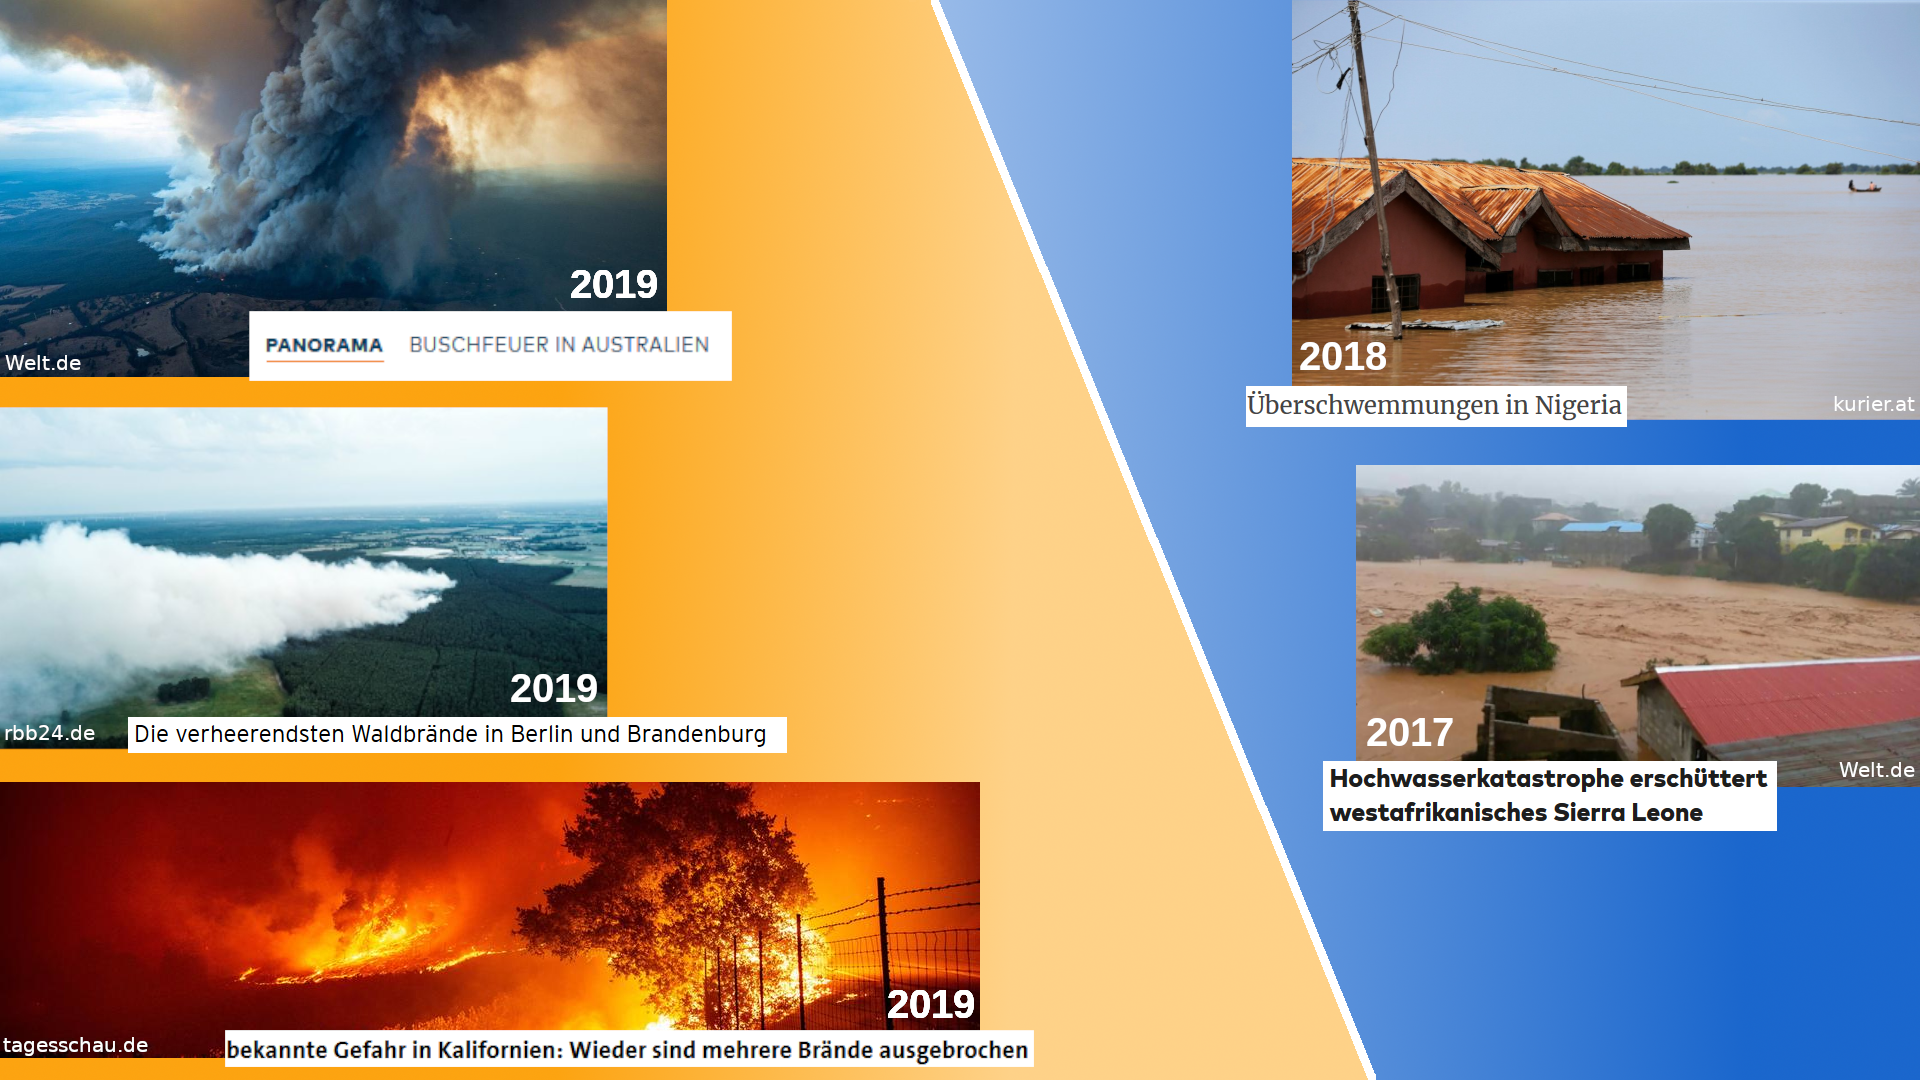
\includegraphics[width=0.9\linewidth]{bilder/CurrentSituation}
		\end{figure}

		\note{
			Wetterereignisse der letzten drei Jahre
			\begin{itemize}
				\item[2017] Hochwasserkatastrophe in Sierra Leone durch bis du dreifach höheren Regenfall als üblich, keine Unwetterwarnung der Regierung, unkontrollierte Entwaldung, Müllverstopfte Kanalisation, etc.
				\item[2018] Überschwemmungen in Nigeria und vielen anderen afrikanischen Ländern, mehrere Millionen Menschen obdachlos
				\item[2019] Buschbrände in Kalifornien, mehr als \SI{1000}{km\squared} (etwa drei mal die Fläche von Dortmund) verbrannt, gehört zu den größten 5 Buschbränden. 4 der größten 5 Brände waren in den letzten 10 Jahren
				\item[2019] Waldbrände in Brandenburg, größte Waldbrände der Geschichte des Landes (etwa 1,5 mal größer als bisher größter),
				etwa \SI{7,50}{km\squared} (etwa die Fläche von Dorstfeld) verbrannt.
				\item[2019] Buschfeuer in Australien, \SI{186000}{km\squared} (\SI{20}{\%} der bewaldeten Fläche Australiens, bzw. \sfrac{1}{2} mal die Fläche von Deutschland) verbrannt, etwa 1 Mrd. Tiere getötet, Rauch auch in Argentinien und Chile spührbar, wird Black Summer genannt.
				\item[2020] zu warmer und trockener Sommer in Deutschland \SI{1,9}{\celsius} über dem Mittel der Referenzperiode 1961 bis 1990, Waldbrände und Hurrikans in den USA, etc.
				\item[$\rightarrow$] Beobachtung extremer Wetterereignisse
			\end{itemize}
		}
	\end{frame}

\begin{frame}
	\frametitle{Aktuelle Nachrichten}
	\begin{figure}
		\centering
		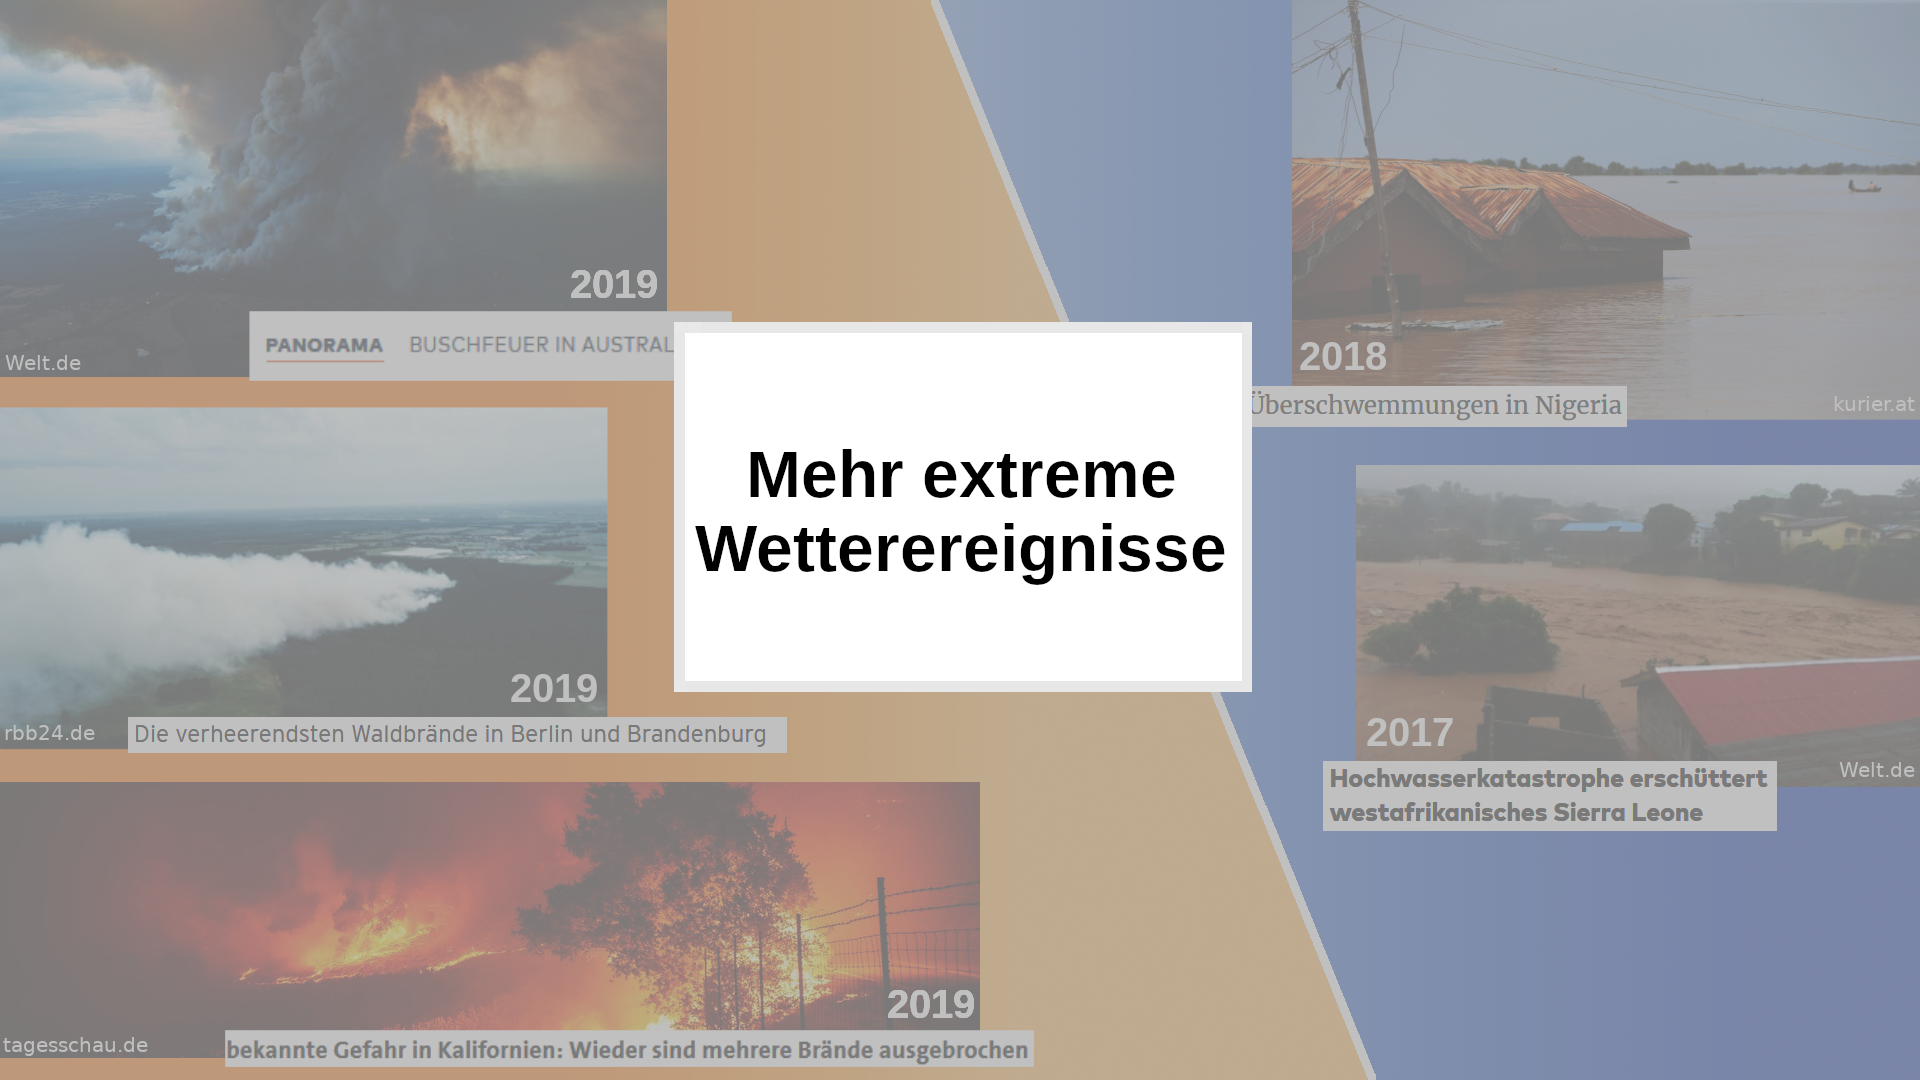
\includegraphics[width=0.9\linewidth]{bilder/CurrentSituation_Conclusion}
	\end{figure}
\end{frame}

\begin{frame}
	\frametitle{Aktuelle Nachrichten}
	\begin{figure}
		\centering
		\begin{tikzpicture}
			\node[anchor=south west,inner sep=0] (image) at (0,0) {
				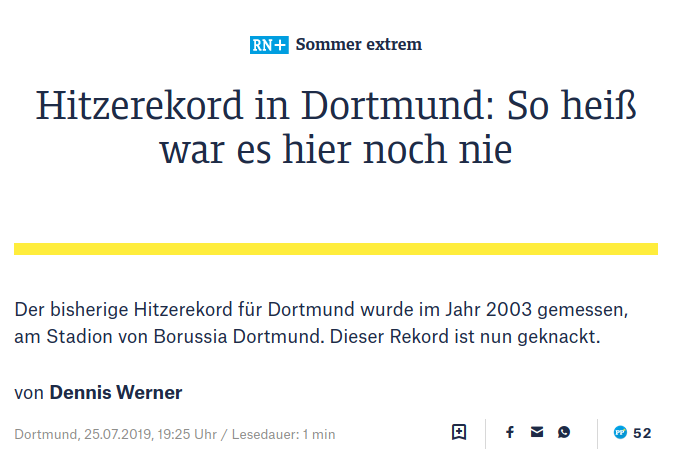
\includegraphics[width=0.7\linewidth]{bilder/dortmund}};
			\begin{scope}[x={(image.south east)},y={(image.north west)}]
				\draw[red,ultra thick,rounded corners] (0.12,0.0475) rectangle (0.23,0.1);
			\end{scope}
		\end{tikzpicture}
	\end{figure}
	\begin{center}
		\textbf{Auch bei uns}
	\end{center}
	\note{
	\begin{itemize}
		\item Man muss gar nicht so weit gehen, in Dortmund ist es genau so (2019)
		\item Extrem Ereignisse lassen sich nicht ausschließlich auf den Klimawandel zurück führen
		\item Statistische Modelle ermöglichen es aber heute zu zeigen, dass Extremereignisse durch den Klimawandel mit einer viel höheren Wahrscheinlichkeit auftreten.
	\end{itemize}
	\vspace{1em}
	Wie sieht das nun global tatsächlich aus?
	}
\end{frame}

% "es war doch immer schon im Sommer warm"


\begin{frame}[t]
	\frametitle{Warming Stripes}
	% Abbildung der Warming Stripes: Die Entwicklung ist wirklich dramatisch

	% Farbskala erklären
	\begin{figure}
		\centering
		\vspace{-1em}
		\begin{tikzpicture}
			\node[anchor=south west,inner sep=0] (image) at (0,0) {
			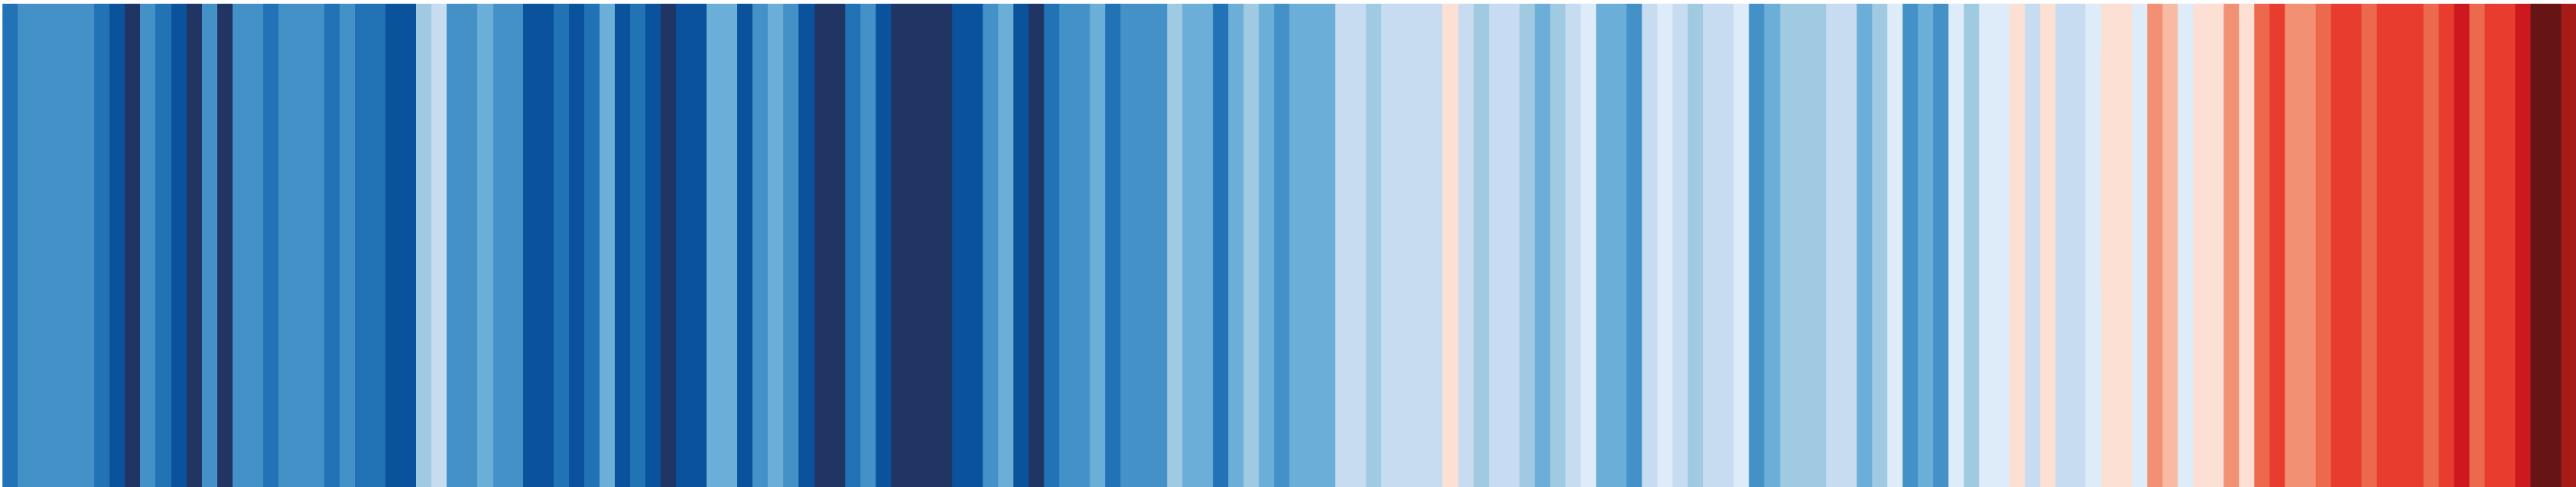
\includegraphics[width=\linewidth]{bilder/s4f-warming-stripes}};
			\begin{scope}[x={(image.south east)},y={(image.north west)}]
				\only<1|handout:1>{\draw[thick,->] (0.0, -0.1) -- (1.0, -0.1) node[anchor=north west] {Zeit};}
				% +/- 0.0058 shifts by one year
				\only<2|handout:0>\fill[gray, opacity=0.7] (0.00,0.003) rectangle (0.3875+0.0058,0.99);
				\only<2|handout:0>\fill[gray, opacity=0.7] (0.3933+0.0058,0.003) rectangle (1.00,0.99);
				\only<3|handout:0>\fill[gray, opacity=0.7] (0.00,0.003) rectangle (0.3875-25*0.0058+0.0025,0.99);
				\only<3|handout:0>\fill[gray, opacity=0.7] (0.3933+5*0.0058+0.0005,0.003) rectangle (1.00,0.99);
				\only<4|handout:0>\fill[gray, opacity=0.7] (0.00,0.003) rectangle (0.3875+5*0.0058+0.0065,0.99);
				\only<4|handout:0>\fill[gray, opacity=0.7] (0.3933+36*0.0058-0.0003,0.003) rectangle (1.00,0.99);
				\only<5|handout:0>\fill[gray, opacity=0.7] (0.00,0.003) rectangle (0.3875+37*0.0058-0.0003,0.99);
				\only<5|handout:0>\fill[gray, opacity=0.7] (0.3933+67*0.0058-0.002,0.003) rectangle (1.00,0.99);
				\only<6|handout:2>\fill[gray, opacity=0.7] (0.00,0.003) rectangle (0.3875+68*0.0058-0.002,0.99);
				\only<6|handout:2>\fill[gray, opacity=0.7] (0.3933+98*0.0058-0.0035,0.003) rectangle (1.00,0.99);
				\only<7|handout:0>{\draw[thick,->] (0.0, -0.1) -- (1.0, -0.1) node[anchor=north west] {Zeit};}
			\end{scope}
	\end{tikzpicture}
		\caption{Die \textit{Warming Stripes}}
		\label{fig:s4f-warming-stripes}
	\end{figure}
	\only<1|handout:1>{
	\begin{itemize}
		\item Jeder Balken repräsentiert eine Jahr aus der Periode 1850-2017
		\item Blau = kälter als der Mittelwert, Rot=Wärmer
		\item Je dunkeler die Farbe, desto extremer die Abweichung vom Mittelwert
		\item Die Trend geht klar zu höheren Temperaturen
		\item Übrigens auch das Logo der Scientists 4 Future
	\end{itemize}
	\begin{center}
		\url{https://s4f-dortmund.github.io/}
	\end{center}
	}
	\only<3|handout:0>{
		\begin{figure}
			\centering
			\vspace{-1em}
			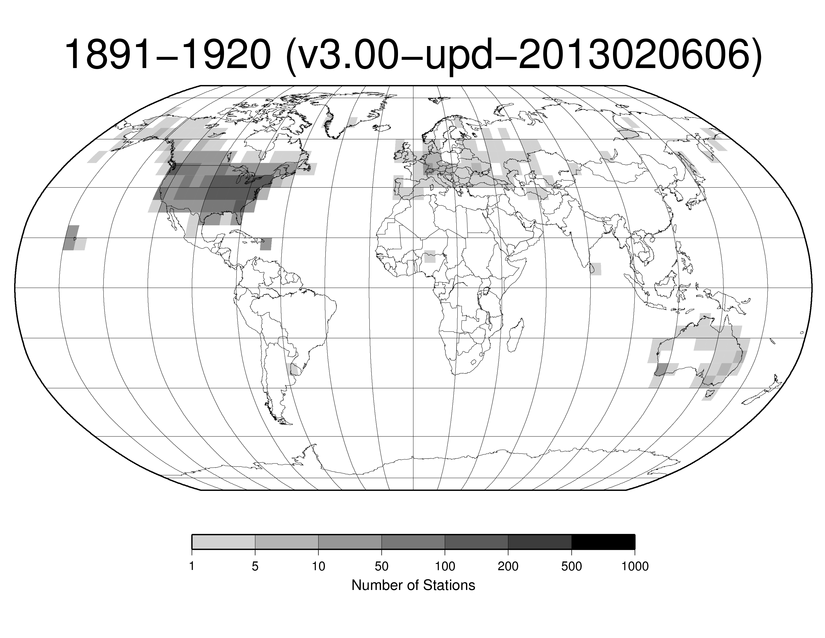
\includegraphics[trim={0cm 1.5cm 0cm 3cm}, clip, width=.425\textwidth]{bilder/Global_Historical_Climate_Network_Daily/station-counts-1891-1920-temp.png}
			\vspace{-1em}
			\caption{Wetterstationen in der Periode 1891 - 1920 die zehn Jahre lang
							 Wetterdaten übertragen haben, Quelle: Global Historical Climate Network}
		\end{figure}
	}
	\only<4|handout:0>{
		\begin{figure}
			\centering
			\vspace{-1em}
			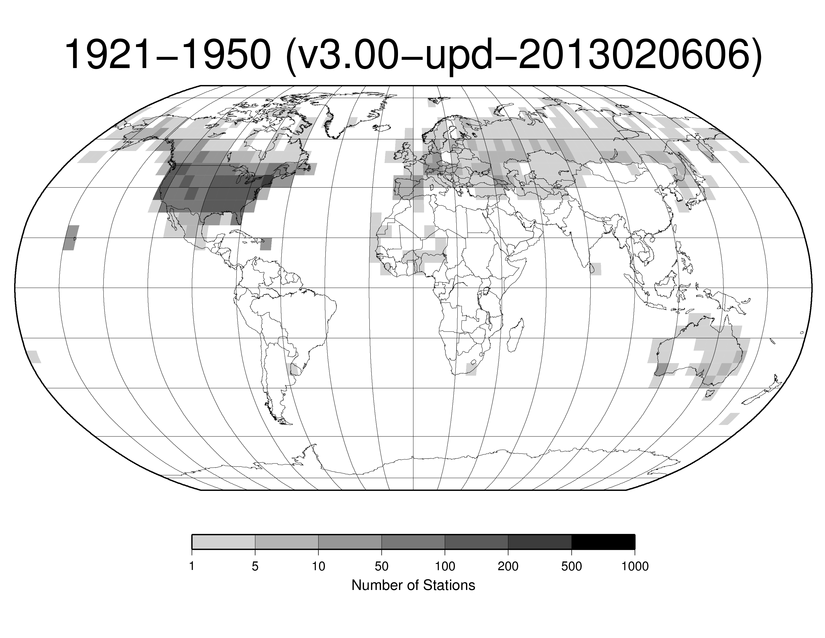
\includegraphics[trim={0cm 1.5cm 0cm 3cm}, clip, width=.425\textwidth]{bilder/Global_Historical_Climate_Network_Daily/station-counts-1921-1950-temp.png}
			\vspace{-1em}
			\caption{Wetterstationen in der Periode 1921 - 1950 die zehn Jahre lang
							 Wetterdaten übertragen haben, Quelle: Global Historical Climate Network}
		\end{figure}
	}
	\only<5|handout:0>{
		\begin{figure}
			\centering
			\vspace{-1em}
			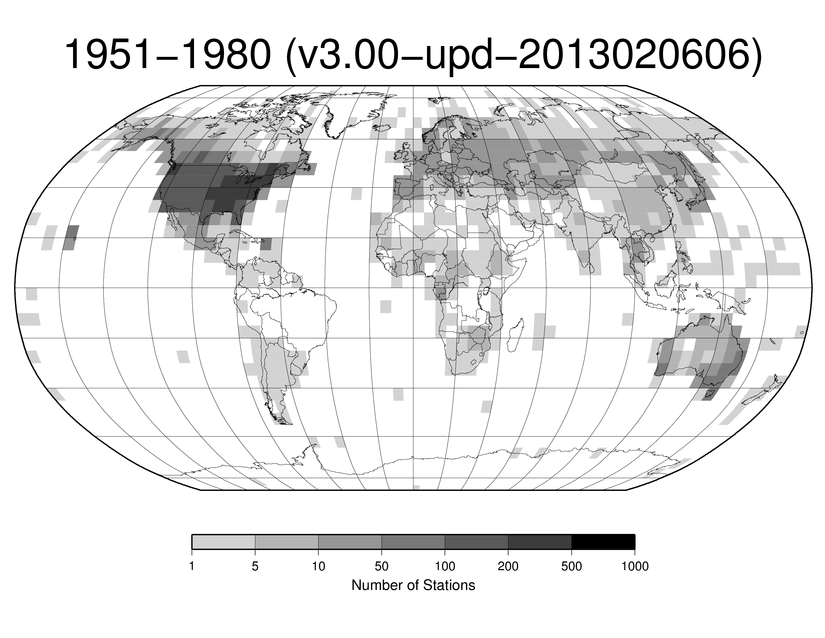
\includegraphics[trim={0cm 1.5cm 0cm 3cm}, clip, width=.425\textwidth]{bilder/Global_Historical_Climate_Network_Daily/station-counts-1951-1980-temp.png}
			\vspace{-1em}
			\caption{Wetterstationen in der Periode 1951 - 1980 die zehn Jahre lang
							 Wetterdaten übertragen haben, Quelle: Global Historical Climate Network}
		\end{figure}
	}
	\only<6|handout:2>{
		\begin{figure}
			\centering
			\vspace{-1em}
			\includegraphics[trim={0cm 1.5cm 0cm 3cm}, clip, width=.425\textwidth]{bilder/Global_Historical_Climate_Network_Daily/station-counts-1981-2010-temp.png}
			\vspace{-1em}
			\caption{Wetterstationen in der Periode 1981 - 2010 die zehn Jahre lang
							 Wetterdaten übertragen haben, Quelle: Global Historical Climate Network}
		\end{figure}
	}
	\only<7|handout:0>{
	\begin{itemize}
		\item Jeder Balken repräsentiert eine Jahr aus der Periode 1850-2017
		\item Blau = kälter als der Mittelwert, Rot=Wärmer
		\item Je dunkeler die Farbe, desto extremer die Abweichung vom Mittelwert
		\item Die Trend geht klar zu höheren Temperaturen
		\item Das Logo der Scientists 4 Future
	\end{itemize}
	\begin{center}
		\url{https://s4f-dortmund.github.io/}
	\end{center}
	}

	\note<1>{
	\begin{itemize}
		\item[] Warming Stripes sind globale Zusammenfassung für ein Großteil der verfügbaren Temperaturdaten (auch S4F Logo)
		\item[] Jeder Balken Jahresmittelwert globaler Luft- und Wassertemperaturen
		\item[] Bei Interesse: Daten auf unserer Homepage verlinkt (auch für verschiedene Orte verfügbar)
	\end{itemize}
	Wie sieht die Zusammensetzung der Daten aus?
	}
	\note<2>{
	\begin{itemize}
		\item[1916] Letzte große Antarktis-Expedition (Endurance-Expedition) Leitung: Ernest Shackleton. Ziel: Den Kontinent durchqueren. Expedition scheiterte. Besonderes: alle Mitglieder unter widrigsten Umständen überlebt.
		\item[] Albert Einstein veröffentlicht die allgemeine Relativitätstheorie.
		\item[] immer mehr Wetterstationen -> genauere Messungen möglich.
	\end{itemize}
	}
	\note<3-6>{
	Immer ein 30 Jahrezeitraum hervorgehoben (später: Definition Klima)
	\begin{itemize}
		\item[vor 1891] Kaum Wetterstationen, 1-5 Stationen pro Quadrant an US-Küsten, Zentraleuropa und austalischer Ostküste
		\item[ab 1891]	Stationen die zehn Jahre lang täglich Wetterdaten übertrugen, Hier:  Temperatur (auch: Niederschlag)
		\item[] USA 50-100 Stationen pro Quadrant, Europa 1-5 Stationen, Australien 1-10 Stationen an der Küste
		\item[] Restliche Welt vereinzelt Stationen
		\item[ab 1921] Canada und Russland mit 1-5 Stationen abgedeckt
		\item[] Erste Stationen in Afrika
		\item[ab 1951] China, Indien, Argentinien, Großteile von Afrika mit 1-5 Stationen
		\item[] Australien, Europa und Teile Russlands mit 5-10 Stationen
		\item[ab 1981] Abdeckung verbessert, doch große Flächen Brasiliens, Grönlands und der Demokratischen Republik Kongo nicht abgedeck, immer noch Lücken
	\end{itemize}
	}
	\note<7>{
	Wir haben verstanden:
	\begin{itemize}
		\item[] Wie sich die globale Lufttemperatur im Laufe der Jahre verändert hat
		\item[] Wie die Lufttemperatur global gemessen wird
		\item[] Was jeder Balken in den Warming Stripes bedeutet
	\end{itemize}
	\vspace{1em}
	Gibt es Fragen?
	\vspace{1em}
	Wie wird die Zukunft aussehen?
	}
\end{frame}

\begin{frame}
	\frametitle{Warming Stripes}
	% Extrapolation der Warming Stripes
	\begin{figure}
		\centering
		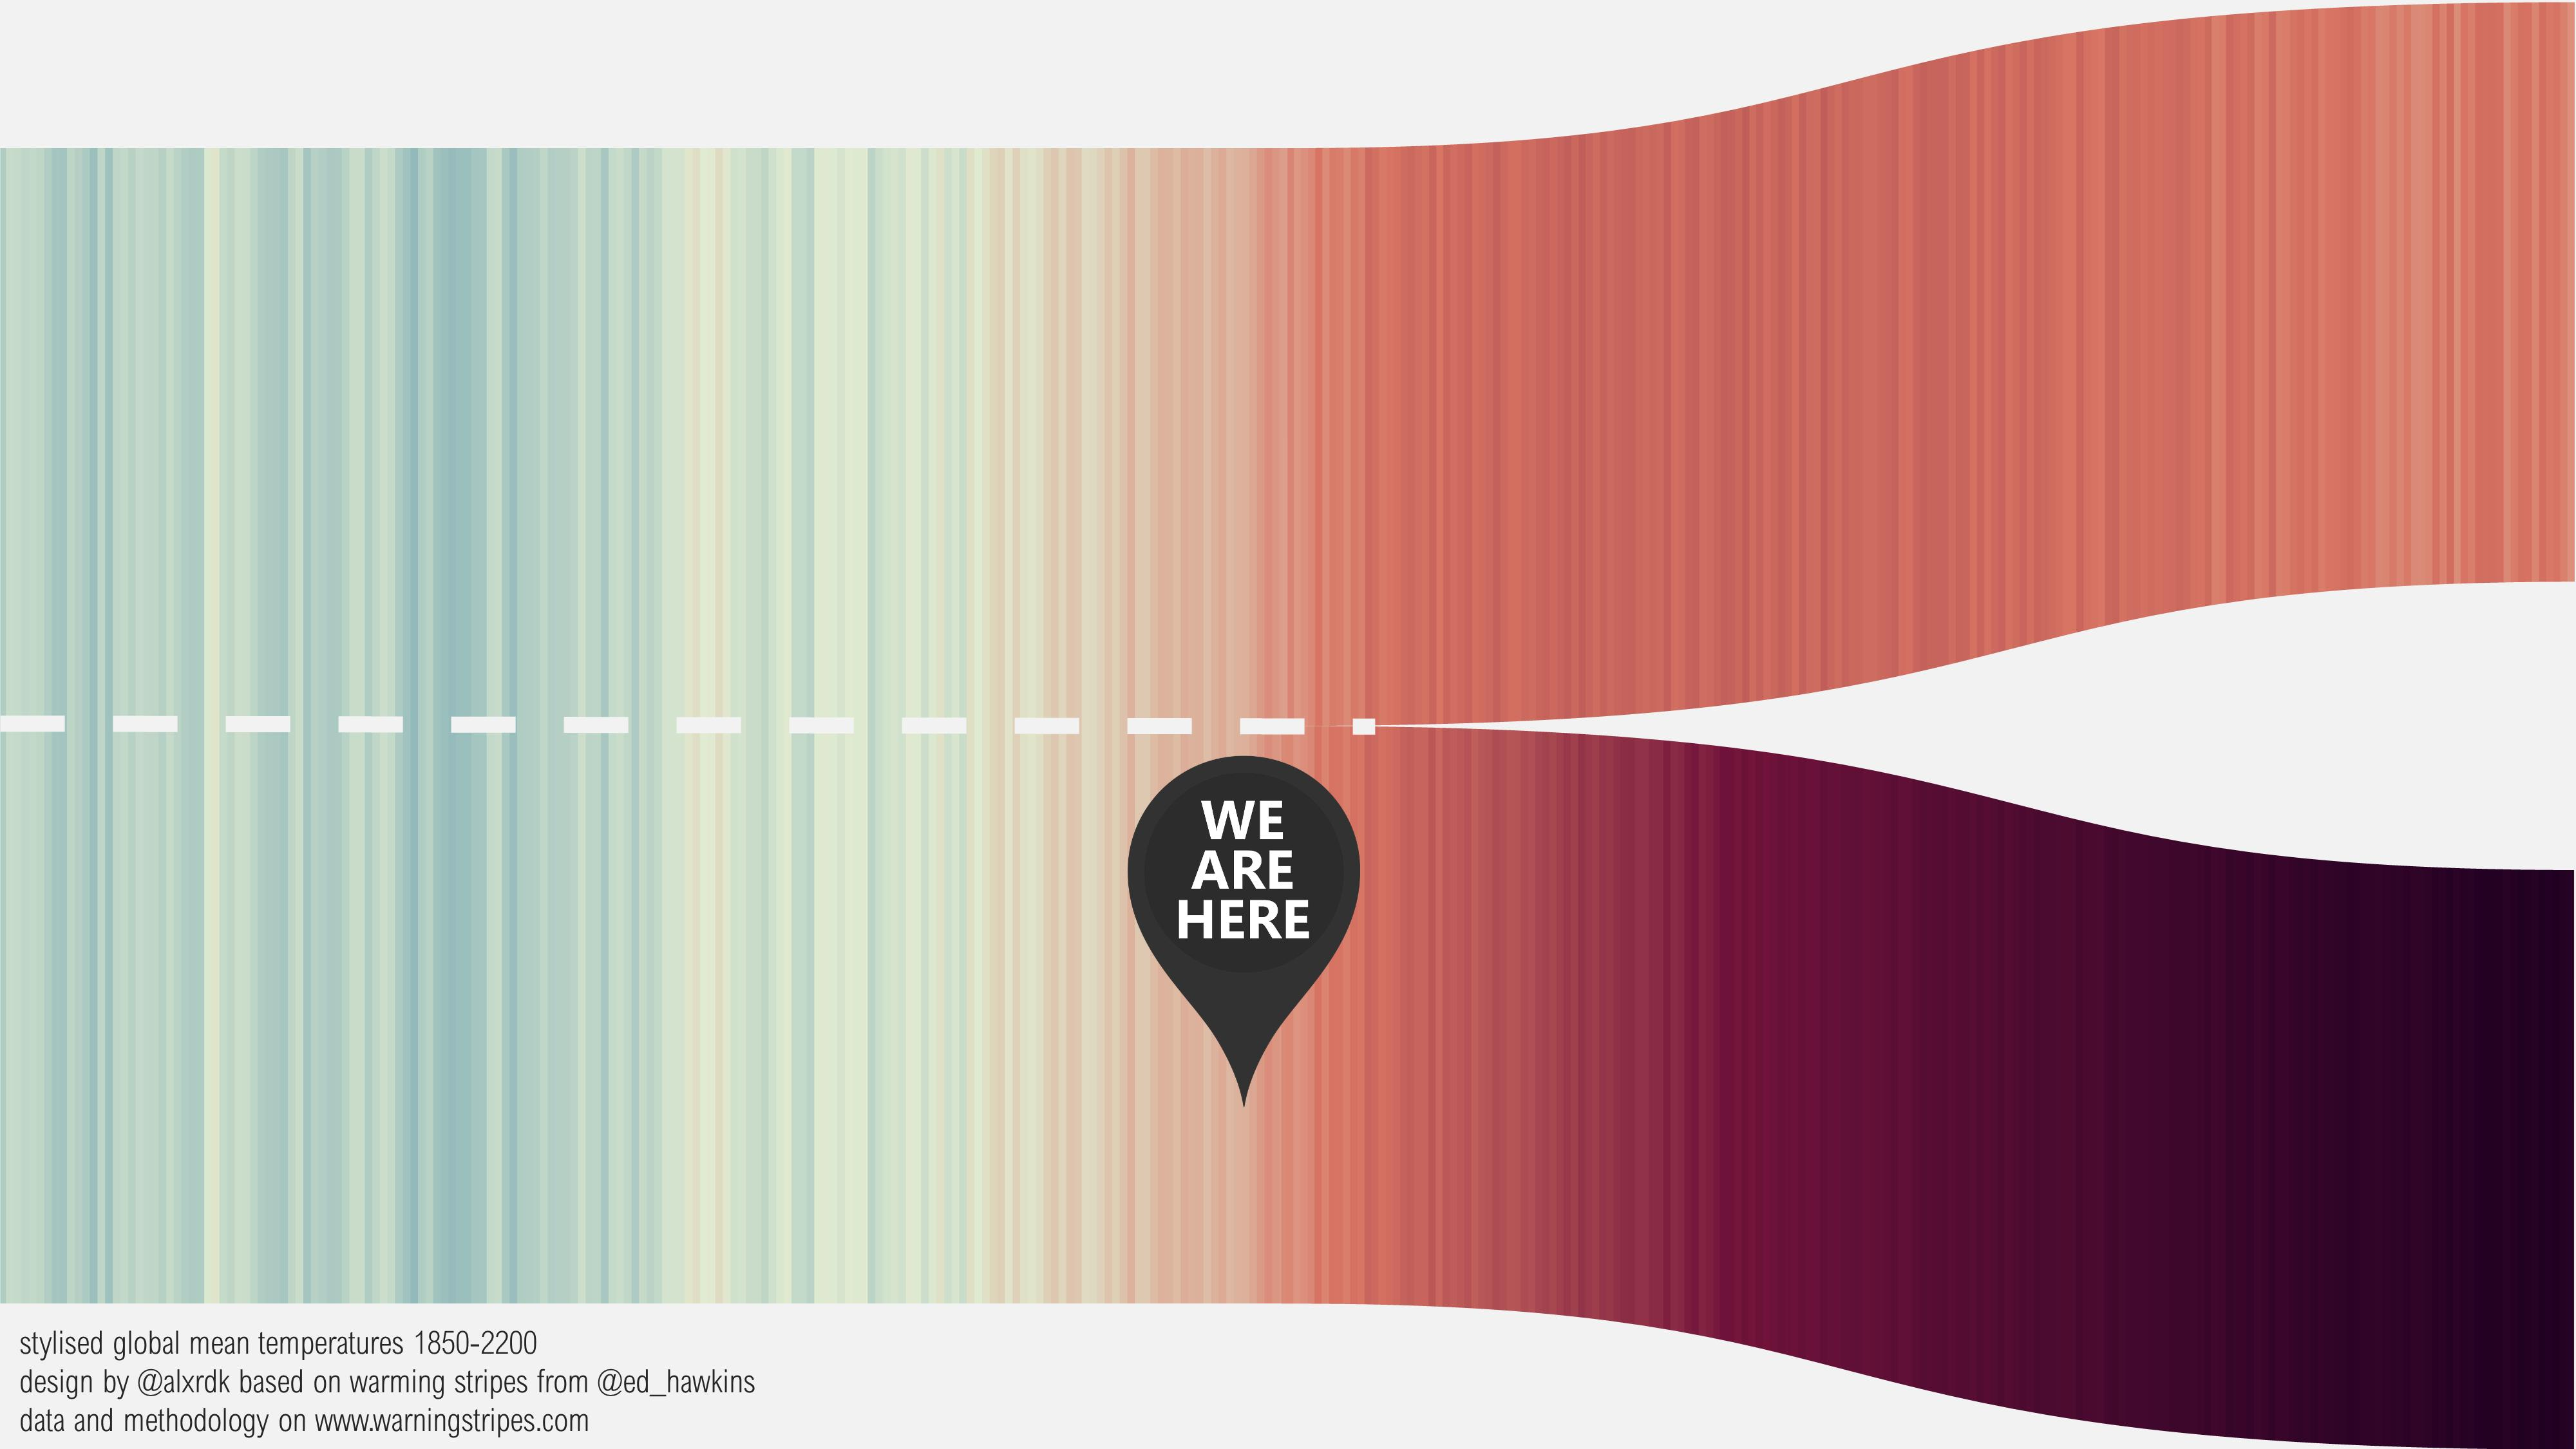
\includegraphics[width=0.55\linewidth]{bilder/warming_stripes_zukunft}
		\caption{Extrapolation der \textit{Warming Stripes} basierend auf Modellannahmen}
	\end{figure}
	\begin{itemize}
		\item In der Zukunft wird es sehr wahrscheinlich zu einer weiteren Erwärmung kommen
		\item Man kann statistische Prognosen für die Zukunft auf Basis von Modellrechnungen erstellen
		\item Der genaue Trend und die maximale Erwärmung hängen aber davon ab, was wir heute und in den nächsten Jahren tun!
	\end{itemize}

\end{frame}

	\subsection{Definition von Wetter und Klima}

\begin{frame}
	% TODO: Wetter vs. Klimadaten Dortmund: zB Osterwetter vs klassisches Niederschlags-Temperatur-Diagramm anfertigen

	% TODO: Daten dazu beim dwd oder bei der Stadt Dortmund Stichwort Opendata -Weather bzw. Witterung

	%TODO: Campuswetter der TU NICHT nutzbar, da urheberrechtlich geschützt
	\frametitle{Wetter und Klima}
	\begin{columns}[onlytextwidth]
		\begin{column}[t]{0.49\linewidth}
			\textbf{Wetter}\\
			\textit{\enquote{ist der physikalische Zustand der Atmosphäre an einem bestimmten Ort zu einem \alert{bestimmten Zeitpunkt} oder in einem kurzen Zeitraum.}}
			\begin{itemize}
				\item Gekennzeichnet durch Ist-Werte von Temperatur, Luftfeuchtigkeit, Niederschlag, ...
				\item Ist was wir täglich mit unseren Sinnen erleben
			\end{itemize}
		\end{column}%
		\begin{column}[t]{0.49\linewidth}
			\textbf{Klima}\\
			\textit{\enquote{ist der mittlere Zustand der Atmosphäre an einem bestimmten Ort über einen \alert{längeren Zeitraum.}}}
			\begin{itemize}
				\item Gekennzeichnet durch statistische Mittelwerte (circa 30 Jahre) der selben Größen
				\item Ist entscheidend für die Entwicklung der Ökosysteme
			\end{itemize}
		\end{column}%
	\end{columns}
	\pause
	\bigskip
	\begin{center}
		Das (durchschnittliche) Wetter macht das Klima, \\
		das Klima bestimmt das (wahrscheinliche) Wetter.
	\end{center}

	\vfill
	\tiny{Zitate von \url{https://www.umweltbundesamt.de/service/uba-fragen/was-ist-eigentlich-klima}}

	\note{
	Klima
	\begin{itemize}
		\item Auch definiert als Zustand des klimatischen Systems, Weltorganisation für Meterologie (WMO)
		\item Betrachtung verschiedener Parameter wie Temperatur, Niederschlag, Windgeschwindigkeiten (WMO)
		\item Betrachtet werden u.a. Mittelwert, Abweichung und Wahrscheinlichkeit des Auftretens extremer Ereignisse z.B. Dürren %M.Latif, Klimawandel und Klimadynamik S. 11
		\item Aus dem Griechischen: \textit{klinein} $\equiv$ neigen $\rightarrow$ Neigung der Erdachse
	\end{itemize}
	\vspace{1em}
	Beispiel
	\begin{itemize}
		\item[] Gut bekannt sind die Jahreszeiten
		\item[] Eine Jahreszeit ist das mittlere Wetter zu der Jahreszeit
		\item[] Ganz einfach gesprochen: wärmer im Sommer und kälter im Winter
		\item[Frage] Woher kommen die Jahreszeiten?
	\end{itemize}
	}

\end{frame}

\begin{frame}
	\frametitle{Klima - Neigung der Erdachse}
	\begin{figure}
		\centering
		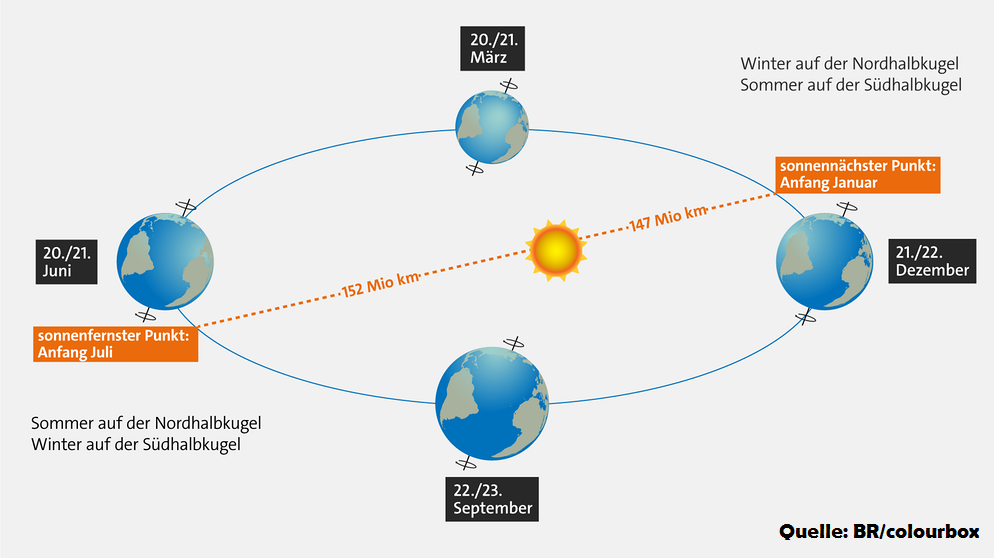
\includegraphics[width=0.7\linewidth]{bilder/Erdumlaufbahn_DWD.png}
		\caption{Neigung der Erdachse als Ursache für die Jahreszeiten, Quelle: Deutscher Wetterdienst}
	\end{figure}

	\begin{itemize}
		\item Die Neigung der Erde ist entscheidend für die Sonneneinstrahlung auf der Erde
		\item [$\rightarrow$] und damit verantwortlich für die Jahreszeiten und das Klima auf der Nord und Südhalbkugel
	\end{itemize}

	\note{
	\begin{itemize}
		\item[] Erde rotiert um die Sonne in einem variablen Abstand von 147 mio. bis 152 mio. Kilometern
		\item[] Ebenso dreht sich die Erde und um die eigene Achse
		\item[]	Neigung der Erdachse zur Ebene der Erdbahn um die Sonne momentan etwa \SI{23,5}{°}
		\item[$\rightarrow$] Jahreszeiten, denn der Winkel der Sonneneinstrahlung ist entscheidend für den lokalen Energieeintrag
		\item[] Ist nur für kurze Zeiträume richtig
		\item[$\rightarrow$] Milankovic-Zyklen in den 1930er Jahren entdeckt
	\end{itemize}
	}
\end{frame}

\begin{frame}
\frametitle{Klima - Eiszeitzyklen}
\begin{figure}
	\centering
	\begin{tikzpicture}
		\node[anchor=south west,inner sep=0] (image) at (0,0) {
		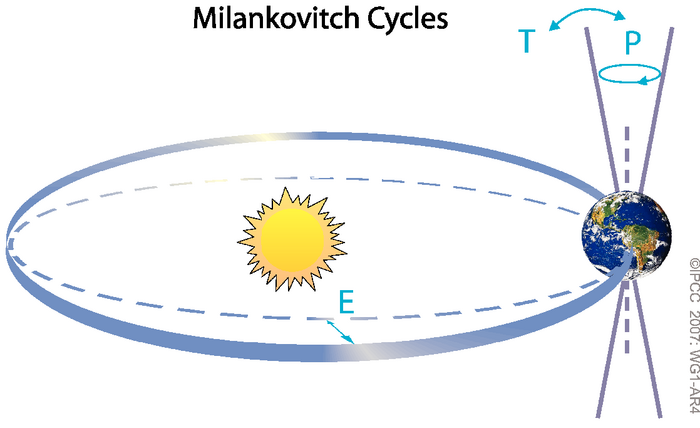
\includegraphics[width=.55\linewidth]{bilder/milankovitch_IPCC2007_AR4.png}};
		\begin{scope}[x={(image.south east)},y={(image.north west)}]
			\onslide<2>\draw[red,ultra thick] (0.495,0.25) circle (1.75em);
			\onslide<3>\draw[red,ultra thick] (0.79,0.92) circle (1.75em);
			\onslide<4>\draw[red,ultra thick] (0.9,0.85) circle (1.75em);
		\end{scope}
	\end{tikzpicture}
	\caption{Milankovitch-Zyklen: Periodische Änderungen der Erdbahnparameter, Quelle: IPCC 2007, WG1, Kapitel 6}
\end{figure}
\begin{itemize}
	\item[E] Veränderung der Ausdehnungsrichtung der Erdbahn (Exzentrizität)% - aktuell: 0,017 perfekter Kreis bei 0, leicht elliptisch bei 0,05
	\item[T] Veränderung des Neigungswinkels der Erdachse (eng. tilt)
	\item[P] Schwankung der Erde um die Erdachse (Präzession) % da die Erde keine perfekte Kugel ist
	\item[$\rightarrow$] verursachen Eiszeitzyklen, sowie deren Warm- und Kaltphasen
	\item[$\rightarrow$] langfristiger Einfluss auf das Klima
\end{itemize}

\note{
\begin{itemize}
	\item[] Milankovic in den 1930er Jahren, Eiszeitzyklen
	\item[] Exzentrizität: Erdbahn variiert
	\begin{itemize}
		\item[] Periode: etwa 1 mio. Jahre, variiert zwischen \num{0,002} und \num{0,05}
		\item[] Momentan: \num{0,017}, perfekter Kreis bei 0, leicht elliptisch bei \num{0,05}.
		\item[] Ursache: Störung durch die anderen Planeten des Sonnensystems, im wesentlichen Jupiter und Saturn.
		\item[] Folge: Solare Einstrahlung wird um weniger als \SI{1}{W\per \square m} geändert.
	\end{itemize}
	\item[] Neigung der Erdachse
	\begin{itemize}
		\item[] Periode: \num{41000} Jahre, Auslenkung zwischen \SIrange{22}{24,5}{°}
		\item[] Momentan: \SI{23,5}{°}
		\item[] Ursache: Gravitationseinfluss der anderen Himmelskörper im Sonnensystem
		\item[] Folge: Verstärkt oder schwächt jahreszeitliche Unterschiede.
		\item[] Keine Veränderung der gemittelten, jährlichen Sonneneinstrahlung.
	\end{itemize}
	\item[] Präzession der Erde, taumeln um die eigene Achse
	\begin{itemize}
		\item[] Periode: etwa \num{20000} Jahre
		\item[] Ursache: Die Erde ist keine perfekte Kugel.
		\item[] Folge: Jahreszeiten treten nicht immer im gleichen Bahnpunkt der Erdbahnellipse auf.
	\end{itemize}
\end{itemize}
}
\end{frame}


\begin{frame}
	\frametitle{Klimaänderung}
	\begin{block}{Klimaänderung}
		Erkennbare (messbare) Änderung Klimas über einen gewissen Zeitraum (z.B. 30 Jahre) %M.Latif Klimawandel und Klimadynamik S. 13
		Spürbar durch Änderung atmosphärischer Größen wie der Temperatur
	\end{block}

	\uncover<2->{
	\begin{figure}
		\centering
		\begin{tikzpicture}
			\node (image1) {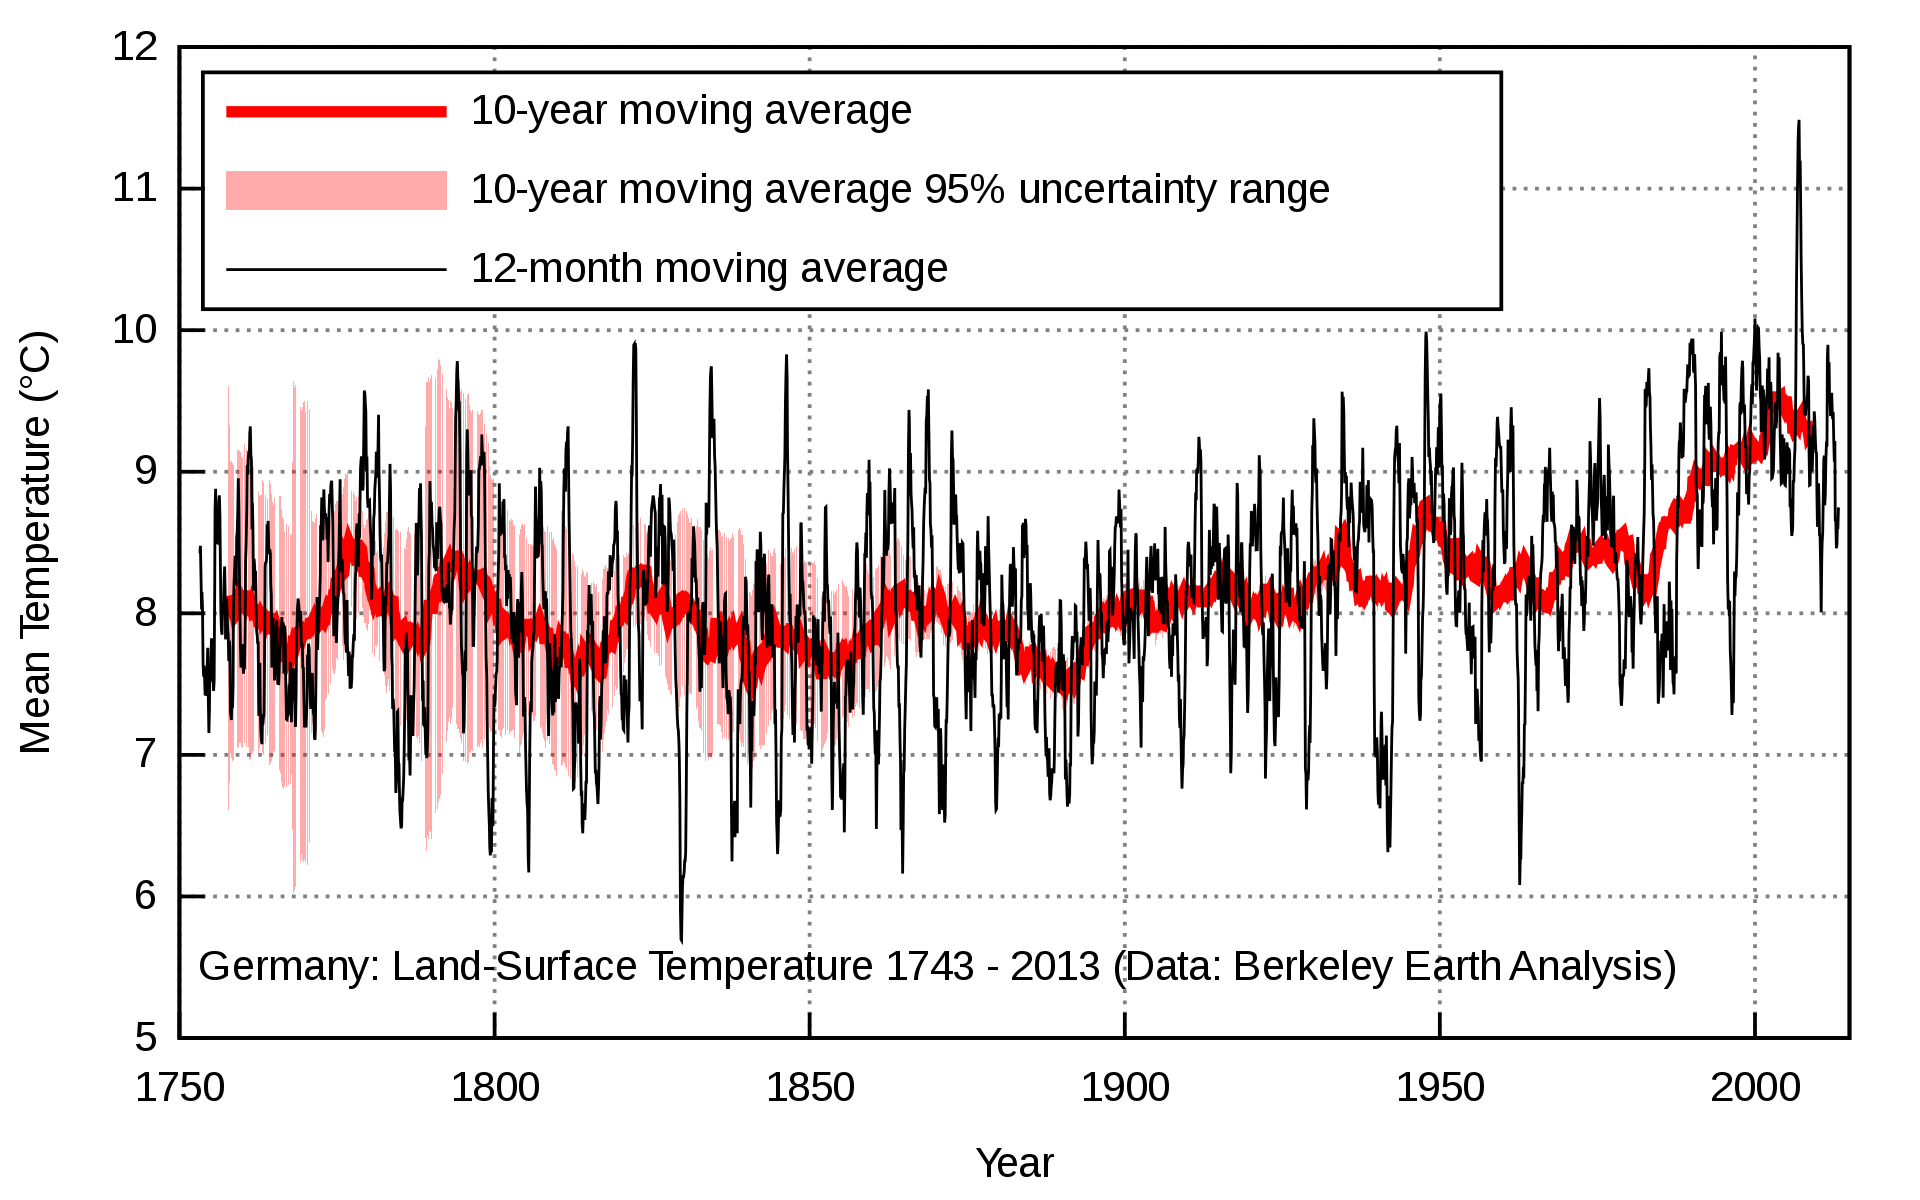
\includegraphics[width=0.6\linewidth]{%
				bilder/Temp_Deutschland_1743-2013_Berkley_Wiki.png}};
			\onslide<3>\node (image2) at (image1.west) [xshift=-0.9cm]{%
				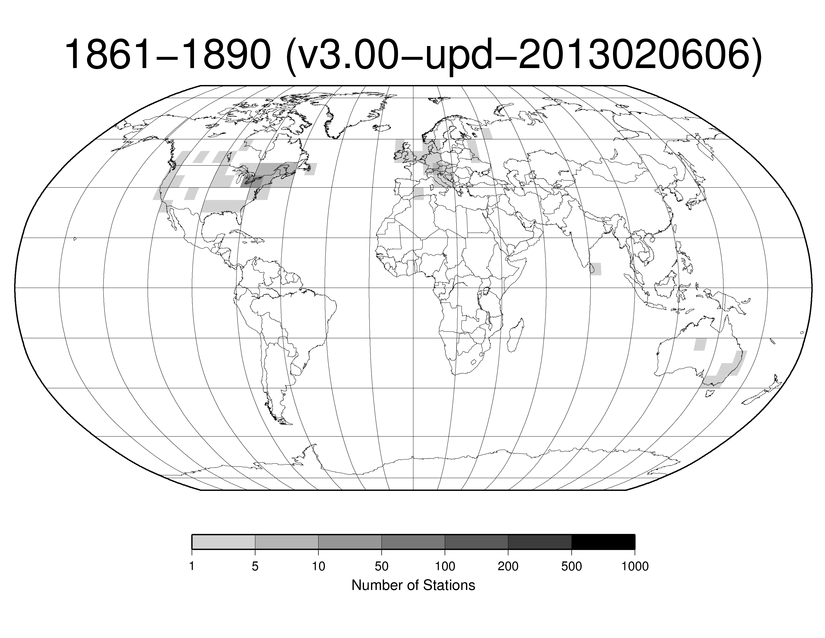
\includegraphics[trim={0cm 1.5cm 0cm 3cm}, clip, width=0.25\linewidth]{%
					bilder/Global_Historical_Climate_Network_Daily/station-counts-1861-1890-temp.png}};
			\onslide<3>\node (image3) at (image1.east) [xshift=1.4cm]{%
				\includegraphics[trim={0cm 1.5cm 0cm 3cm}, clip, width=0.25\linewidth]{%
					bilder/Global_Historical_Climate_Network_Daily/station-counts-1981-2010-temp.png}};
	  \end{tikzpicture}
		\caption{Entwicklung der mittleren Jahrestemperaturen in Deutschland, Quelle: Wikipedia, Daten: Berkeley Earth Surface Temperature Project}
	\end{figure}
	}

	%TODO Bild mit 30 Jahre moving average erstellen
	\note{
	Definition: Eine Klimaänderung ist eine erkennbare (messbare) Änderung Klimas über einen gewissen Zeitraum (z.B. 30 Jahre), pürbar durch Änderung atmosphärischer Größen wie der Temperatur
	\begin{itemize}
	 	\item[] mittlere Temperaturen in Deutschland pro Jahr von 1743 bis 2013
	 	\item[] 10 Jahre moving average, Fluktuation, aber Temperaturanstieg
	 	\item[] 30 Jahre moving average, weniger Schwankungen, kleiner, aber  deutlicher Temperaturanstieg
		\item[] in hellrot: Unsicherheit auf den gleitenden Durchschnitt nimmt ab (Erinnerung an Dichte der Wetterstationen)
	 \end{itemize}
	 \vspace{1em}
	 \begin{itemize}
	   \item[] Zentrale Frage: Was bestimmt das Klima?
	   \item[] Wie ist ein Erdklima möglich?
	   \item[] Grundlage bildet die Sonne. Aber was ist der Unterschied zu unseren Nachbarn?
	   \item[] Mittlere Oberflächentemperaturen: Venus \SI{464}{°C}, Mars \SI{-55}{°C}
	   \item[$\rightarrow$] Die Erde hat eine Atmosphäre
	   \item[] Die Atmosphäre sorgt dafür, dass eine gewisse Menge der Sonnenenergie auf der Erde verbleibt
	   \item[] lebenfreundliche Temperaturen werden auf der Erde erreicht
	 \end{itemize}
	}

\end{frame}

	\subsection{Die Strahlungsprozesse der Erde}

\begin{frame}
	\frametitle{Aufbau der Atmosphäre}
	\begin{figure}
		\centering
    \begin{columns}
      \column{0.1\linewidth}
      \column{0.5\linewidth}
      \begin{tikzpicture}
		    \node[anchor=south west,inner sep=0] (image) at (0,0) {
        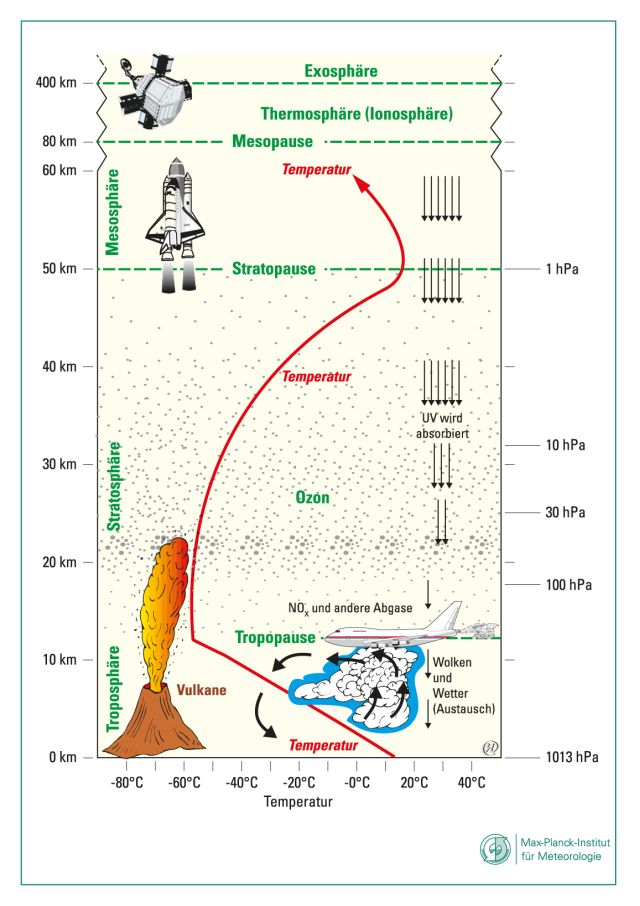
\includegraphics[width=.85\linewidth]{bilder/atmosphaere-stockwerkaufbau_bildungsserver_hh.jpg}};
        \begin{scope}[x={(image.south east)},y={(image.north west)}]
        \onslide<2|handout:0>\draw[red,ultra thick,rounded corners] (0.05,0.15) rectangle (0.95,0.285);
        \onslide<3|handout:0>\draw[red,ultra thick,rounded corners] (0.05,0.285) rectangle (0.95,0.715);
        \onslide<4|handout:0>\draw[red,ultra thick,rounded corners] (0.05,0.715) rectangle (0.95,0.855);
        \onslide<5|handout:0>\draw[red,ultra thick,rounded corners] (0.05,0.855) rectangle (0.95,0.96);
    \end{scope}
      \end{tikzpicture}
      \column{0.3\linewidth}
        \caption{Schematischer Aufbau der Atmosphäre, Quelle: Bildungsserver Hamburg}
      \column{0.1\linewidth}
    \end{columns}
	\end{figure}

  \note<2>{
    Troposphäre, \SIrange{10}{12}{km}
    \begin{itemize}
      \item[] \SI{80}{\%} der Atmosphärenmasse, enthält fast allen Wasserdampf
      \item[] Hier finden alle wetterrelevanten Phänomene statt
      \item[] ersten \SIrange{1}{2,5}{km} starker Einfluss der Erdoberfläche
      \item[] Jetstreams an oberer Grenze, kein Transport von H$_2$0 von Troposphäre in die Stratosphäre
    \end{itemize}
		}
	\note<3>{
    Stratosphäre, \SIrange{12}{50}{km}
    \begin{itemize}
      \item[] Anstieg der Ozonkonzentration sorgt für Temperaturanstieg
      \item[] Die Prozesse hier (Strahlung, Dynamik, Chemie) relevant für Klima in der Troposphäre
    \end{itemize}
		}
	\note<4>{
    Mesosphäre, \SIrange{50}{80}{km}
    \begin{itemize}
      \item[] Stetige Temperaturabnahme
    \end{itemize}
		}
	\note<5>{
    Thermosphäre, \SIrange{80}{400}{km}
    \begin{itemize}
      \item[] extrem geringe Teilchendichte, Weltram fängt bei \SI{100}{km} an (NASA), Bremswirkung der Atmosphäre aber auch bei \SI{400}{km} Höhe noch spührbar (ISS wird regelmäßig von andockenden Raumschiffen auf ihre Bahn zurück geschoben)
    \end{itemize}
    Exosphäre, \SIrange{400}{1000}{km}
    \begin{itemize}
      \item[] quasi Vakuum
    \end{itemize}
    Grenzen nicht hart, Troposphäre z.B.
    \begin{itemize}
      \item[] 10-12 km im Durchschnitt
      \item[] 8 km an den Polen
      \item[] 17-18 km in den Tropen
    \end{itemize}
  }
\end{frame}

%Übergang: Ohne die Atmosphäre hätten wir auf der Erde eine durchschnittliche Temperatur von -18 Grad, durch die Atmosphäre und die atmosphärischen Gase ist es aber im Mittel etwa etwa 35 Grad wärmer -> 15 Grad

\begin{frame}
  \frametitle{Strahlungshaushalt}

  \begin{figure}
  	\centering
    \begin{tikzpicture}
      \node[anchor=south west,inner sep=0] (image) at (0,0){
  	   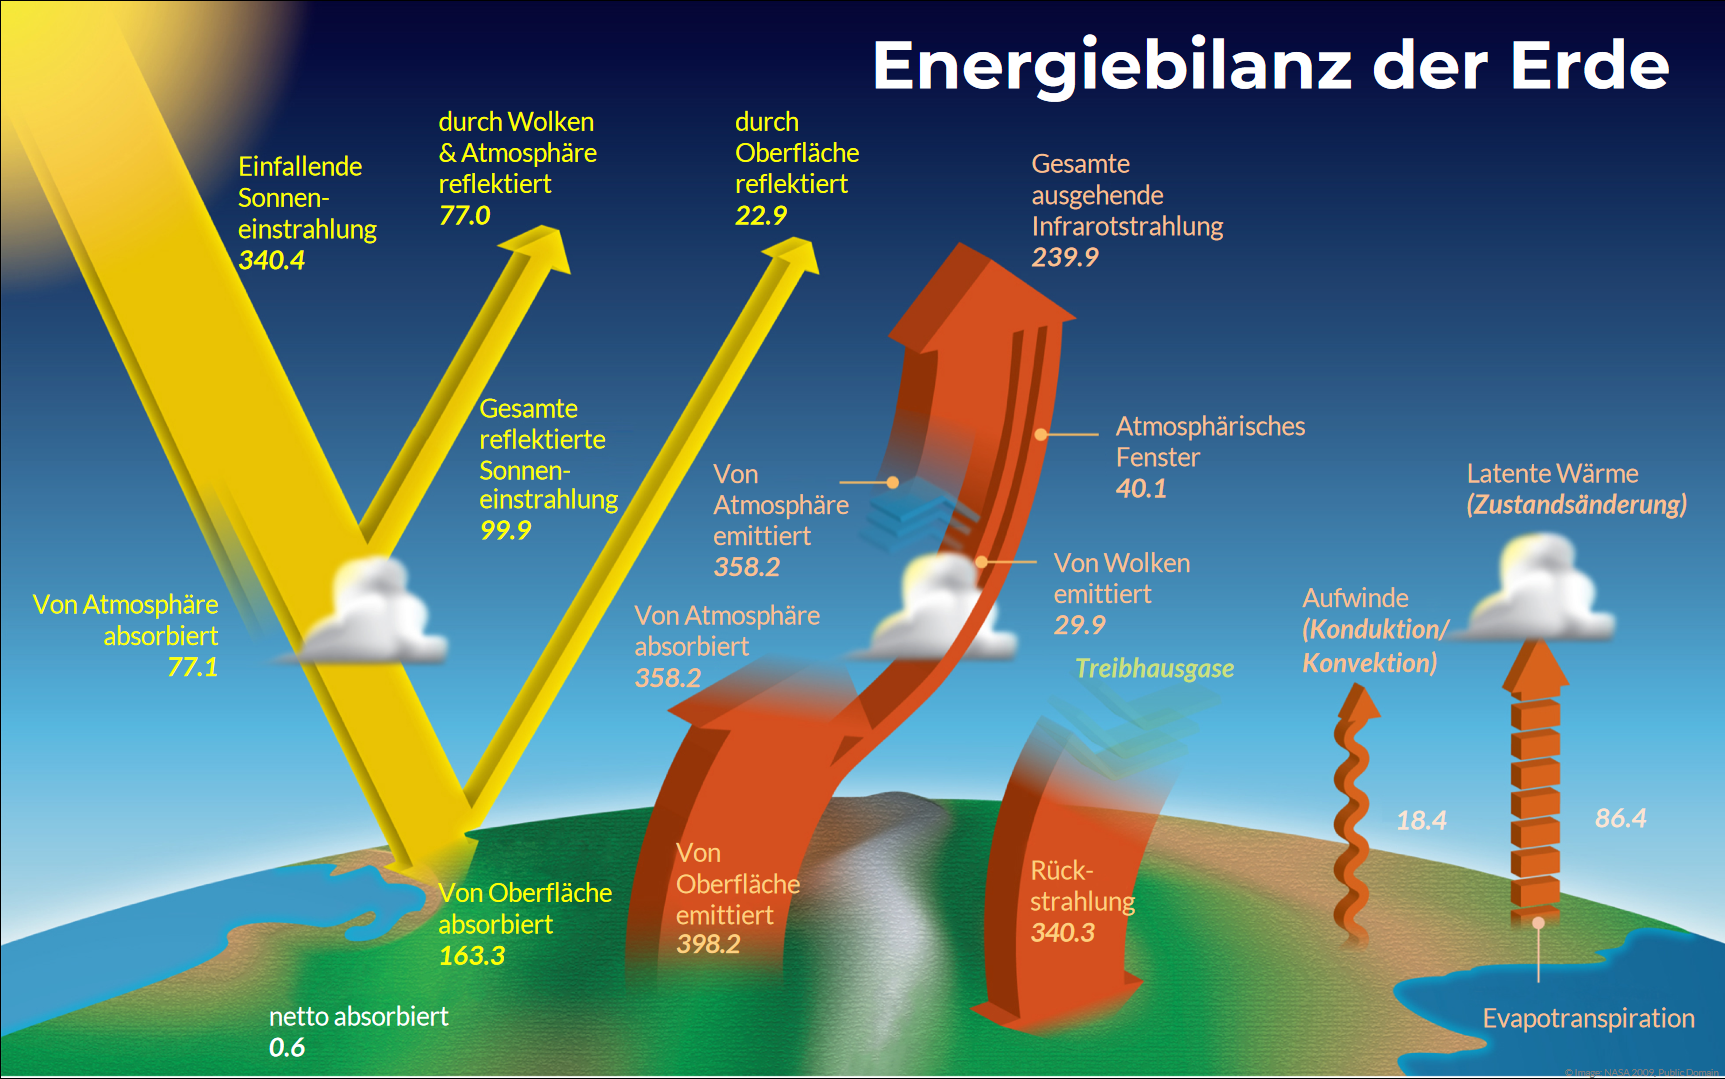
\includegraphics[width=0.8\linewidth]{bilder/Energiebilanz_der_Erde_NASA.png}};
      \uncover<2->{
        \node[anchor=south west, text=red] (text) at (4.7, 3.235) {\scriptsize\textbf{\rule[0.5ex]{2em}{0.55pt}\;\num{169.9}}};
      }
    \end{tikzpicture}
  	\caption{Strahlungshaushalt der Erde, Angaben in W/m$^2$, Quelle: NASA nach Kiehl und Trenberth 1997, Übersetzung: S4F} % Die Abbildung ist in den Folien der S4F Vertiefung zum Klimawandel (S.21) aber dort leider nur spärlich referenziert. Annahme: Jemand der S4F hat dieses Bild Übersetzt und dem Abbildungs-Pool hinzugefügt.
  \end{figure}

  %Abbildung für Strahlungshaushalt einfügen z.B: vom Bildungsserver Hamburg https://bildungsserver.hamburg.de/atmosphaere-und-treibhauseffekt/2069644/atmosphaere-strahlungshaushalt-artikel/
  % bzw. vom den S4F materialien: http://files.scientists4future.org/Themen/2.%20Klimawandel/Als%20PDFs/S4F-03%20Klima%20Vertiefung%202020-01-31.pdf
  % oder vom IPCC AR5 Figure 2.11
  \note<1->{
  \begin{itemize}
    \item[] Ohne die Atmosphäre hätten wir eine durchschnittliche Oberflächentemperatur von \SI{-18}{°C}
    \item[] Mit Atmosphäre (Treibhausgase) ist es im Mittel \SI{33}{°C} wärmer, wir haben eine durchschnittliche Oberflächentemperatur von \SI{15}{°C}
    \item[] Solarkonstante: \SI{1368}{W\per m\squared} oberhalb der Atmosphäre
    \begin{itemize}
      \item[] Zur Erwärmung der Atmosphäre verfügbar: \SI{340}{W\per m\squared} auf Grund der Kugelgestalt und der Nachtseite der Erde
      \item[] rund \SI{70}{\%} der gesamten einfallenden Strahlung werden absorbiert (Atmosphäre (\SI{22}{\%}), Oberfläche (\SI{48}{\%}))
      \item[] rund \SI{30}{\%} der gesamten einfallenden Strahlung werden reflektiert (Wolken und Atmosphäre (\SI{23}{\%}), Erdoberfläche (\SI{7}{\%}))
    \end{itemize}
	\end{itemize}
	}
	\note<2->{
	\begin{itemize}
    \item[] Damit sich die Erde nicht aufheizt, muss die absorbierte Energie wieder abgegeben werden
    \item[$\rightarrow$] Die absorbierte kurzwellige Sonneneinstrahlung wird als langwellige infrarot Strahlung wieder abgegeben (vgl. Eingehend \SI{340}{W\per m\squared} und Ausgehend \SI{100}{W\per m\squared} reflektiert, sowie \SI{240}{W\per m\squared} als IR abgestrahlt)
    \item[] Zusätzlich \SI{340}{W\per m\squared} Rückstrahlung $\rightarrow$ Woher kommen die?
    \begin{itemize}
      \item[] Einergiebilanz der Atmosphäre: \SI{77}{W\per m\squared} Sonneneinstrahlung + \SI{358}{W\per m\squared} Erdeinstrahlung + \SI{18}{W\per m\squared} Aufwinde + \SI{86}{W\per m\squared} latente Wärme - \SI{200}{W\per m\squared} von Wolken und Atmosphäre emittiert = \SI{340}{W\per m\squared} bleiben übrig
      \item[$\rightarrow$] Treibhauseffekt
			\item[$\rightarrow$] zuvor: Exkurs Licht
    \end{itemize}
  \end{itemize}
  }
\end{frame}

	% Fokus auf den Treibhauseffekt, d.h. vorherige Abbildung reduziert um ein paar Energieflüsse  (mitte)
% zB Sonneneinstrahlung- Atmosphärische Reflexion = 235 W/m2
% Die Abbildung zeigt zum einen die Temperatur auf der Erde ohne die Strahlungsbilanz der Erde(links) außerdem nochmal den atmosphärischen Aufbau (rechts)
% In der Mitte ist die Auswirkung der Treibhausgase zu sehen
\subsection{Der Treibhauseffekt}

\begin{frame}
  \frametitle{Treibhauseffekt}
  \only<1|handout:0>{
  \begin{figure}
  	\centering
  	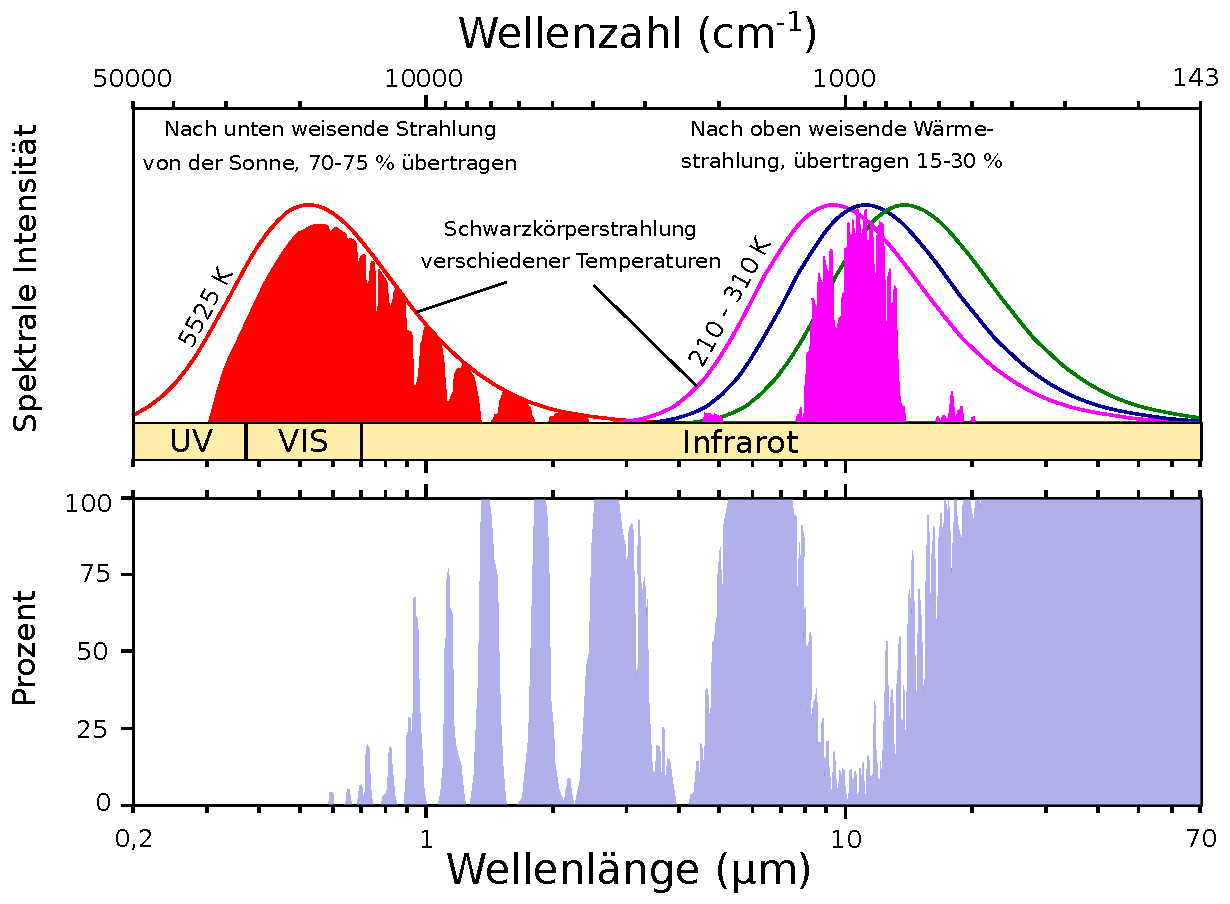
\includegraphics[width=0.7\linewidth]{bilder/Atmospheric_Transmission-H2O.pdf}
    \caption{Absorption und Streuung von Wasser in der Atmosphäre, Quelle: Robert A. Rohde, Global Warming Art project}
  \end{figure}
    }
    \only<2|handout:0>{
    \begin{figure}
    	\centering
    	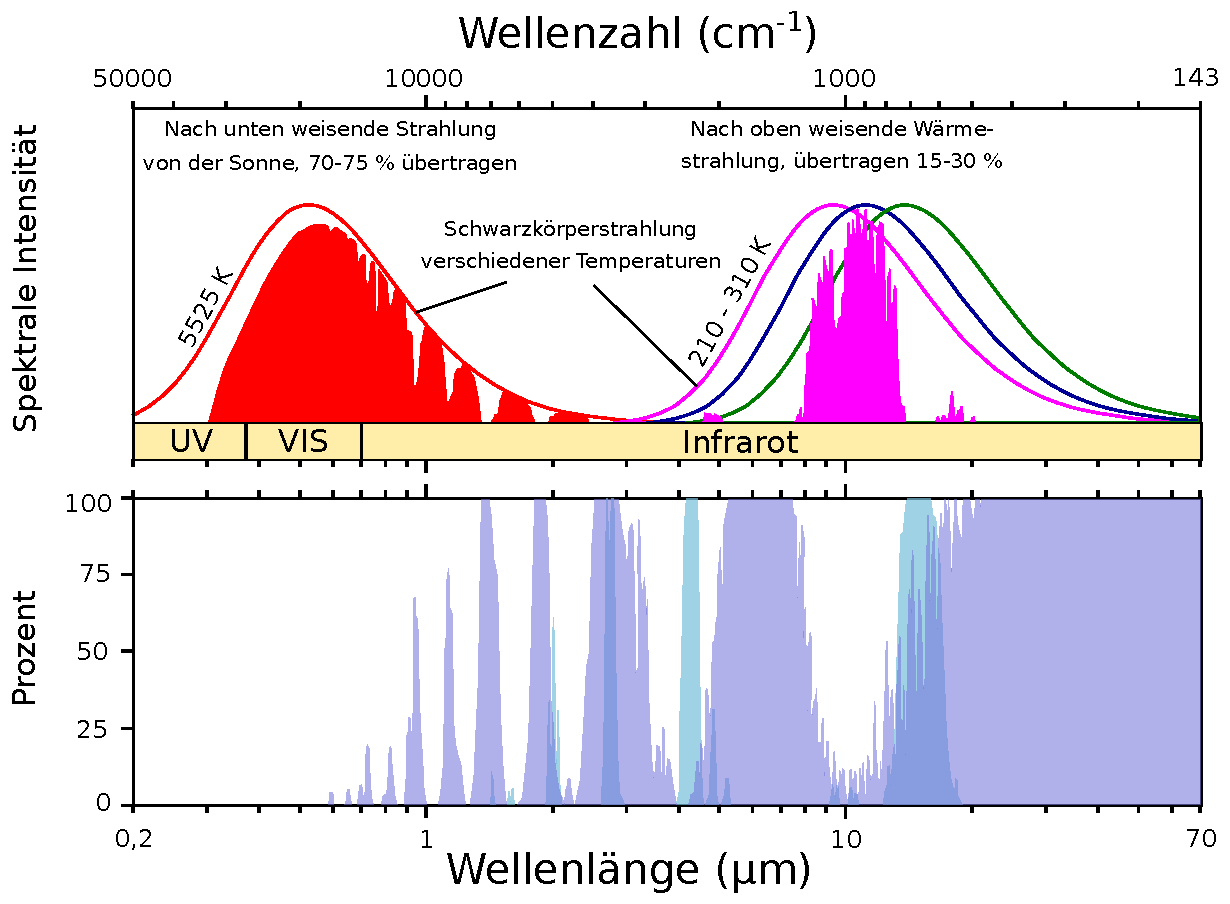
\includegraphics[width=0.7\linewidth]{bilder/Atmospheric_Transmission-H2O-CO2.pdf}
      \caption{Absorption und Streuung von Wasser und CO$_2$ in der Atmosphäre, Quelle: Robert A. Rohde, Global Warming Art project}
    \end{figure}
    }
    \only<3|handout:0>{
    \begin{figure}
    	\centering
    	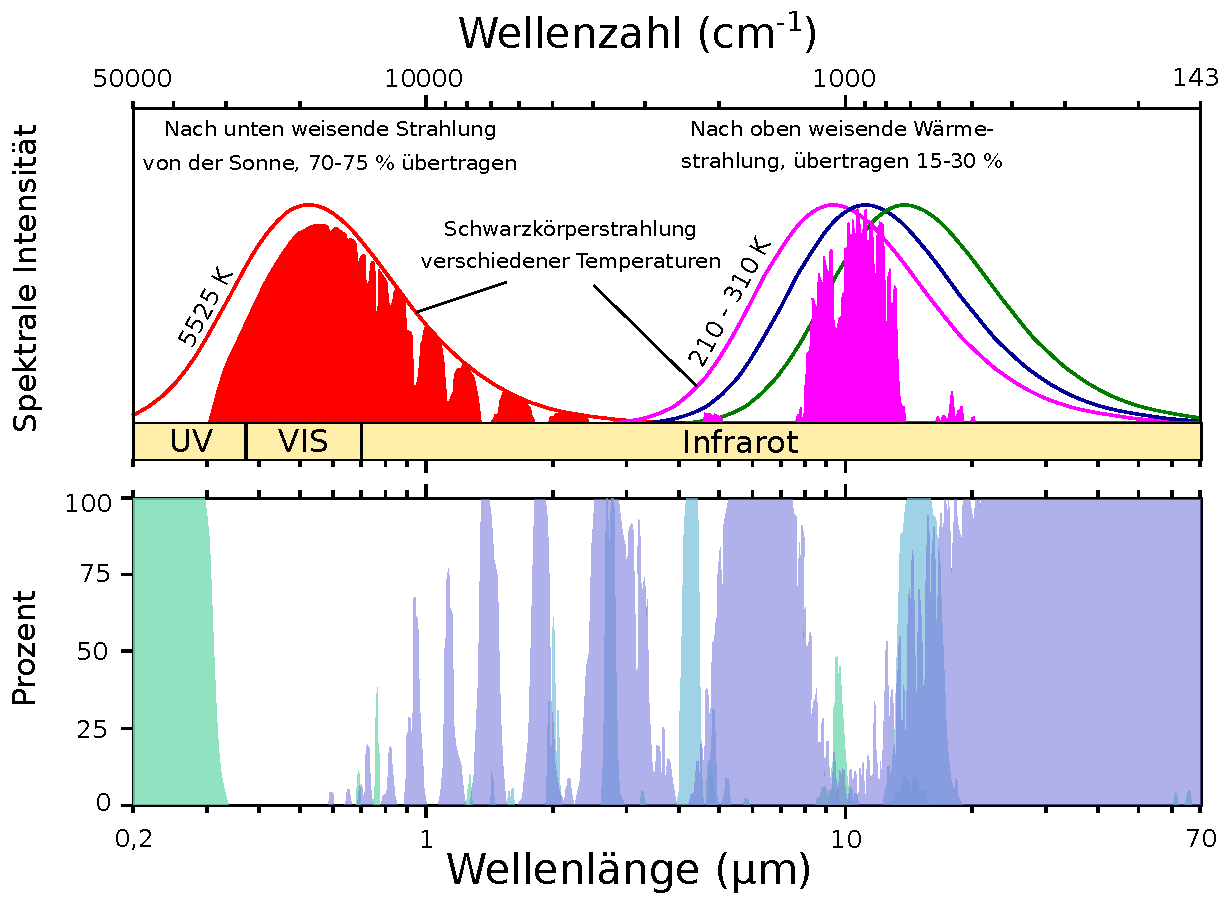
\includegraphics[width=0.7\linewidth]{bilder/Atmospheric_Transmission-H2O-CO2-O2O3.pdf}
    \caption{Absorption und Streuung von Wasser, CO$_2$, sowie Sauerstoff und Ozon in der Atmosphäre, Quelle: Robert A. Rohde, Global Warming Art project}
  \end{figure}
    }
    \only<4|handout:0>{
    \begin{figure}
    	\centering
    	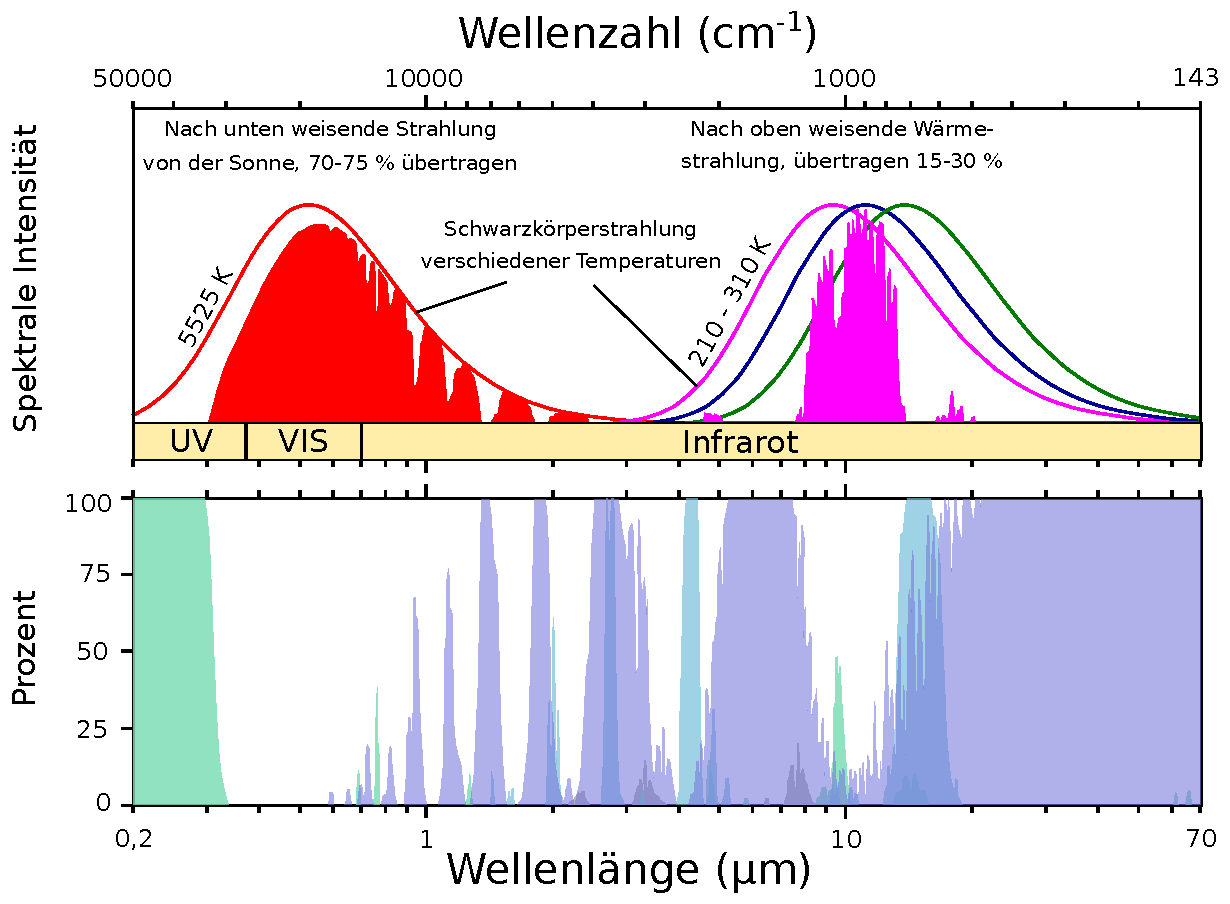
\includegraphics[width=0.7\linewidth]{bilder/Atmospheric_Transmission-H2O-CO2-O2O3-CH4.pdf}
    \caption{Absorption und Streuung von Wasser, CO$_2$, Sauerstoff, Ozon und Methan in der Atmosphäre, Quelle: Robert A. Rohde, Global Warming Art project}
  \end{figure}
    }
    \only<5>{
    \begin{figure}
    	\centering
    	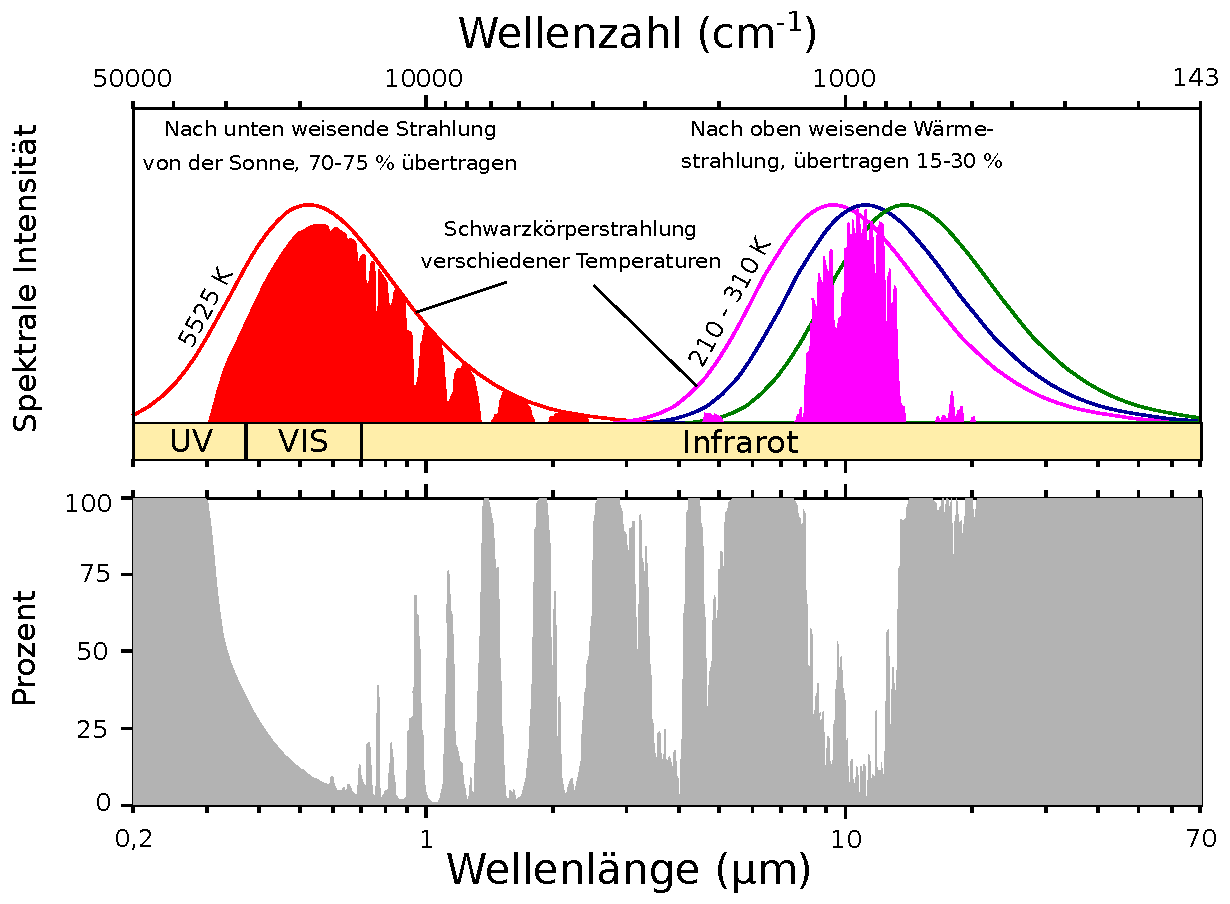
\includegraphics[width=0.7\linewidth]{bilder/Atmospheric_Transmission-all.pdf}
    \caption{Gesamtabsorption und -streuung der Atmosphäre, Quelle: Robert A. Rohde, Global Warming Art project}
  \end{figure}
    }

  \note<1->{
  \begin{itemize}
    \item[] Thermische Ausstrahlung der Erde etwa \SI{240}{W\per m\squared}
    \item[$\rightarrow$] entspricht einer Strahlungstemperatur von etwa \SI{-20}{°C} (Plancksches Strahlungsgesetz, Wärmestrahlung eines schwarzen Körpers)
    \item[] tatsächlich beobachtete Temperatur aber \SI{35}{°C} höher, Wie ist das möglich?
		\item  {\color{red}{Wasserdampf H$_2$O}} -  großer Teil des natürlicher Treibhauseffekt (\SI{60}{\%})
  \end{itemize}
  }
  \note<2->{
  \begin{itemize}
		\item  {\color{red}{Kohlenstoffdioxid CO$_2$}} - entsteht u.A. bei der Nutzung fossiler Brennstoffe (Öl, Kohle, Gas)
    \item[$\rightarrow$] Anstieg auf den Menschen zurückzuführen
  \end{itemize}
  }
  \note<3->{
  \begin{itemize}
    \item  {\color{red}{Ozon O$_3$}} - entsteht bei Reaktion von Auto-Abgasen in der Luft im Sonnenlicht
  \end{itemize}
  }
  \note<4->{
  \begin{itemize}
		\item  {\color{red}{Methan CH$_4$}} - entsteht u.a. bei der Zersetzung von organischem Material
		\item[$\rightarrow$] $>$ 60\,\% der globalen Methan-Emissionen sind auf menschliche Aktivitäten zurückzuführen %ClimateChange Kurs der Uni Helsinki Chapter 1.3.3
  \end{itemize}
  }
  \note<5->{
  \begin{itemize}
		\item  {\color{red}{Distickstoffmonoxid N$_2$O (Lachgas)}} - entsteht beim Abbau von Düngemitteln in der Erde
		\item {\color{red}{fluorierte Treibhausgase (F-Gase)}}
		\item[$\rightarrow$] kommen nicht natürlich vor, sehr treibhauswirksam, verweilen z.T. sehr lange in der Atmosphäre, bis zu 10.000 Jahre, aber kommen nur in sehr geringer Konzentration vor
    \item[] F-Gase: voll halogenierte Fluorkohlenwasserstoffe (FKW, englisch: PFC), teilhalogenierte Fluorkohlenwasserstoffe (HFKW, englisch: HFC), Schwefelhexafluorid (SF6) und Stickstofftrifluorid (NF3).
		\item[] F-Gase kommen in der Natur nicht vor; aber befinden sich u.a. in Gefriertruhen, Klimaanlagen, Feuerlöschern und Dämmstoffen.
	\end{itemize}
  }
\end{frame}

\begin{frame}
	\frametitle{Treibhausgase}
	\begin{figure}
		\centering
    \begin{columns}
      \column{0.7\linewidth}
        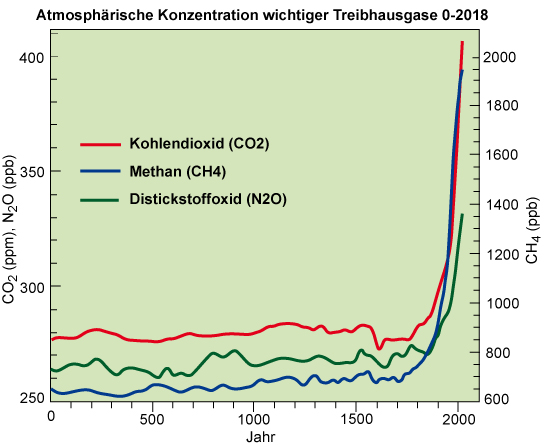
\includegraphics[width=\linewidth]{bilder/Treibhausgase0-aktuell_bildungsserver_hh.jpg}
      \column{0.3\linewidth}
        \caption{Treibhausgaskonzentration in der Atmosphäre, Quelle: Bildungsserver Hamburg}
    \end{columns}
		%Abbildung wie in S.Ranmstorf S.33 -> http://www.pik-potsdam.de/~stefan/Publications/Book_chapters/Der_Klimawandel_Kapitel2.pdf oder direkt im IPCC 2013: https://www.ipcc.ch/report/ar5/wg1/observations-atmosphere-and-surface/ Fig 2.1-2.3
	\end{figure}
\note{
  \begin{itemize}
    \item[] All diesen Stoffen gemeinsam ist ein sehr starker Anstieg der Konzentration seit Beginn der Industrialisierung
    \item[] Der Anstieg ist in absoluten und relativen Zahlen sehr signifikant
    \item[] In dieser Geschwindigkeit ist der Anstieg in der Erdgeschichte beispiellos
    \item[] Die Erhöhung kann im wesentlichen auf menschliche Aktivitäten zurückgeführt werden und setzt sich in Zukunft sehr wahrscheinlich weiter fort
  \end{itemize}
  }
\end{frame}



\begin{frame}
	\frametitle{Treibhausgase - Klimawirksamkeit}
		\begin{figure}
			\begin{columns}
				\column{0.6\linewidth}
				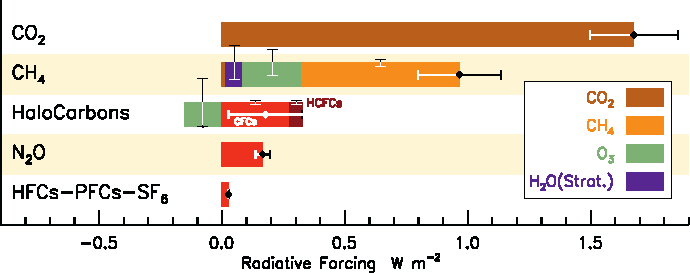
\includegraphics[width=0.9\linewidth]{bilder/radiative_forcings_of_ghg.pdf}
				\column{0.25\linewidth}
				\caption{Strahlungsantrieb der Treibhausgase zwischen 1750 und 2011, Quelle: IPCC 2013 Kapitel 8}
			\end{columns}
		\end{figure}
\begin{itemize}
	\item Die Änderungen des Strahlungsantriebs sind durch den Menschen verursacht (ersichtlich durch den betrachteten Zeitraum und das Emissionsquellen bekannt sind)
	\item CO$_2$, CH$_4$ und N$_2$O zählen zu den langlebigen Treibhausgasen und sind über den Globus verteilt.
	\item Der Grad des wissenschaftlichen Verständnisses über diese ist hoch!
\end{itemize}
\note{
  \begin{itemize}
    \item[] Neben den Treibhausgasen beeinflussen weitere Faktoren den globalen Strahlungsantrieb (Energiebilanz der Erde)
    \item[] Diese sind im allgemeinen gekoppelt, z.B. beim Abschmelzen von Eismassen auf Grund von höherer Temperatur
   	\item[] Manche Faktoren wirken dämpfend auf den Strahlungsantrieb, etwa eine erhöhte Aerosolkonzentration
   	\item[] Der Einfluss der Veränderung der Sonnenaktivität (gerne genannten Argument gegen menschgemachten Klimawandel) ist hingehen vergleichsweise klein
   	\item[] Insgesamt gibt es aber (trotz einiger bestehender Unsicherheiten) eine eindeutige Erhöhung des Stralungsantriebs durch menschliche Aktivitäten
    \item[] Contrails = Condensation Trails
    \item[] O$_3$ ist kontinental bis global verbereitet und das Verständnis ist Mittel
  	\item[] CH$_4$ ist global verbreitet jedoch ist das Verständnis über den Strahlungsantrieb gering.
  	\item[] Das Verständnis sinkt nach Einträgen und daher besonders für die verringernden RF-Faktoren wie Albedo ungewiss. Die Verringerung könnte auch deutlich niedriger liegen, was bedeutet, dass der von den Menschen verursachte Strahlungsantireb sogar noch stärker ist. - Da durch die Erderwärmung und Rußablagerungen auf dem Eis der Albedo-Effekt geschmälert wird, ist das sogar wahrscheinlich.
  	% Ergänzungen aus der Abbildung: https://wiki.bildungsserver.de/klimawandel/index.php/Strahlungsantrieb
  \end{itemize}
  }
\end{frame}


\begin{frame}
	\frametitle{CO$_2$-Äquivalent}

	\begin{block}{Strahlungsantrieb / Radiative Forcing / RF}
		Strahlungsenergie pro Quadratmeter, die durch die Tropopause hindurch kommt \\
		Einheit: \SI{}{\watt\per\square\meter}
	\end{block}

	\begin{block}{CO$_2$-Äquivalent}
		Integral des Strahlungsantriebs eines Treibhausgases über einen bestimmten Zeitraum (meist 100 Jahre) im Verhältnis zu dem von CO$_2$

%		Beitrag eines Treibhausgases zum Treibhauseffekt über 100 Jahre gemessen am Beitrag des $CO_2$
	\end{block}


	\color{gray}\rule{\linewidth}{1pt}

	\color{black}

	2018 lag der Wert an CO$_2$-Äquivalenten in der Atmosphäre bei 496\,ppm (RF: 3,101)\\
	\textit{zum Vergleich: } 1990 waren es noch 417\,ppm (RF: 2,165)\\
	$\rightarrow$ \color{red}{Zuwachs des Strahlungsantriebs um 43\,\% seit 1990}
  \note{
  \begin{itemize}
		\item[] Methan (CH$_4$) ist ca. 30-mal klimawirksamer als CO$_2$
		\item[] Lachgas (N$_2$O) ist 265-mal klimawirksamer als CO$_2$
		\item[] das heißt selbst die deutlich kleinere Menge von ihnen in der Atmosphäre (ppb anstatt ppm) hat einen deutlichen Einfluss
	\end{itemize}
  }
\end{frame}

\begin{frame}
	\frametitle{Klimawirksamkeit der Treibhausgase}
%(Quelle: IPCC 2014, Kapitel 8, Tabelle 8.7) %Treibhauswirksamkeit über 100 Jahre ohne Einbezug der Feedbacks - GWP [..] with and without inclusion of climate–carbon feedbacks (cc fb) in response to emissions of the indicated non-CO2 gases

%TODO Abbildung evtl vereinfachen oder bessere Abbildung finden! Einfluss von SO_2 noch nicht betrachtet und generell zu viele Infos über andere Gase enthalten
% SO_2 könnte Debatte eröffnen, die wir an der Stelle noch nicht führen können
% z.B. Abbildung über Verweildauer in der Atmosphäre IPCC 2014 Kapitel 8 Anhang 8.A
% IPCC 2013 Physical Science Bases
		\begin{figure}
			\centering
			  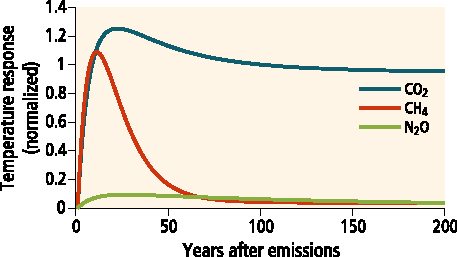
\includegraphics[width=.7\linewidth]{bilder/ghg-forcings-over-time.pdf}
			  \caption{Klimawirksamkeit der Treibhausgase CO$_2$, CH$_4$ und N$_2$O über einen Zeitraum von 200 Jahren, Quelle: IPCC 2014, Kapitel 8}
		\end{figure}

    \note{
    \begin{itemize}
      \item[] auch Methan bleibt vergleichsweise lange klimawirksam
      \item[] Die wichtigsten anthropogehnen Treibhausgase sind CO$_2$, Methan und Lachgas
      \item[] Sie kommen in sehr unterschiedlichen Konzentration in der Atmospähre vor
      \begin{itemize}
        \item Lachgas bspw. circa 1000 mal weniger als CO$_2$
      \end{itemize}
      \item[] Gleichzeitig ist, bedingt durch ihre molekulare Struktur, ihre Treibhauswirkung ebenfalls sehr unterscheidlich
      \item[] Insgesamt ergibt sich eine vergleichbare Wirkung auf den Treibhauseffekt, ein zusätzliche Strahlungsantrieb (Maß für die Änderung der Energiebilanz der Erde) von etwa \SI{0,2}{\watt\per\square\metre} bis \SI{2}{\watt\per\square\metre}
    	\item[] Darüber hinaus verweilen unterschiedliche Stoffe unterschiedlich lang in der Atmosphäre und sind daher auf unterschiedlichen Zeitskalen wirksam
    	\item[] Auf langen Zeitskalen ist CO$_2$ von hoher Bedeutung
      \item[] GWP = Global Warming Potential
      \item[] GTP = Global Temperature Change Potential
      \item[$\rightarrow$] CO$_2$, CH$_4$ und N$_2$O haben über die Zeit die höchste Klimawirksamkeit
      \item[$\rightarrow$] CO$_2$ verliert über den Zeitraum von 100 Jahren kaum an Klimawirksamkeit
      \item[$\rightarrow$] CO$_2$, CH$_4$ und N$_2$O haben über die Zeit die höchste Klimawirksamkeit
		  \item[$\rightarrow$] CO$_2$ verliert über den Zeitraum von 100 Jahren kaum an Klimawirksamkeit
      \item[] Schwefeldioxid ist ein farbloses, schleimhautreizendes, stechend riechendes und sauer schmeckendes, giftiges Gas
    %		auch Methan bleibt vergleichsweise lange klimawirksam\\
      \end{itemize}
      }

\end{frame}

	\begin{frame}
	\frametitle{Eis-Albedo-Rückkopplung}%Rahmstorf, Schellnhuber - Der Klimawandel S. 14
  \begin{center}
	 Reflexion der ankommenden Sonneneinstrahlung durch Eismassen\\[3em]
 \end{center}

	 \begin{columns}[T] % align columns
	 	\begin{column}{.48\textwidth}
	 		\centering
	 		\textbf{Abkühlung}\\
	 		\color{blue}\rule{\linewidth}{4pt}
	 		\color{black}
	 		\color<2->{gray}
	 		je mehr Eismassen\\
	 		$\downarrow$\\
	 		desto mehr wird reflektiert/\\
	 		desto weniger wird absorbiert\\
	 		$\downarrow$\\
	 		desto kälter wird es auf dem Planeten\\
	 		$\downarrow$\\
	 		desto weniger Wasserdampf kann die Atmosphäre aufnehmen\\
	 		$\downarrow$\\
	 		desto geringer wird der Treibhauseffekt
	 	\end{column}%
	 	\hfill%
	 	\begin{column}{.48\textwidth}<2->
	 		\centering
	 		\textbf{Aufwärmung}\\
	 		\color{red}\rule{\linewidth}{4pt}
	 		\color{black}
	 		je weniger Eismassen\\
	 		$\downarrow$\\
	 		desto weniger wird reflektiert/\\
	 		desto mehr wird absorbiert\\
	 		$\downarrow$\\
	 		desto wärmer wird es auf dem Planeten\\
	 		$\downarrow$\\
	 		desto mehr Wasserdampf kann die Atmosphäre aufnehmen\\
	 		$\downarrow$\\
	 		desto stärker wird der Treibhauseffekt
	 	\end{column}%
	 \end{columns}
\note{
\begin{itemize}
	\item[] hier wird die genannten Wechselwirkung unterschiedlicher Faktoren am Beispiel Eis-Albedo Rückkoppelung erläutert
	\item[] Albedo ist im wesentlichen das Reflexionsvermögen eines Körpers auf einer Skala von 0 bis 1, eine hohe Albedo bedeutet viel Reflexion
	\item[] I.a. gibt es viele ähnliche Rückkoppelungen im Klimasystem, z.B. auch bei Landnutzung/Grünflächen und kann im Prinzip sowohl positiv wie negativ sein
	\item[] Negative Rückkoplung führt zu einem stabilen Verhalten, positive Rückkopplung zu schwer kontrolierbarem Anwachsen.
  \end{itemize}
  }

\end{frame}

% "Runterscrollen" / "Zoom" in einer Abbildung von den Atmosphärischen Schichten auf die Erde

	% Abbildung, die nach und nach wächst, mit den erklärten Teilbereichen

% vgl IPCC AR5 climate feedbacks, AR4 chapter 1 basics: carbon cycle
\subsection{Die Faktoren des Klimasystems}

\begin{frame}
  \frametitle{Faktoren des Klimasystems}
  \begin{columns}
	\column{0.7\linewidth}
	\begin{figure}
	 	\centering
    % trim={<left> <lower> <right> <upper>}
	 	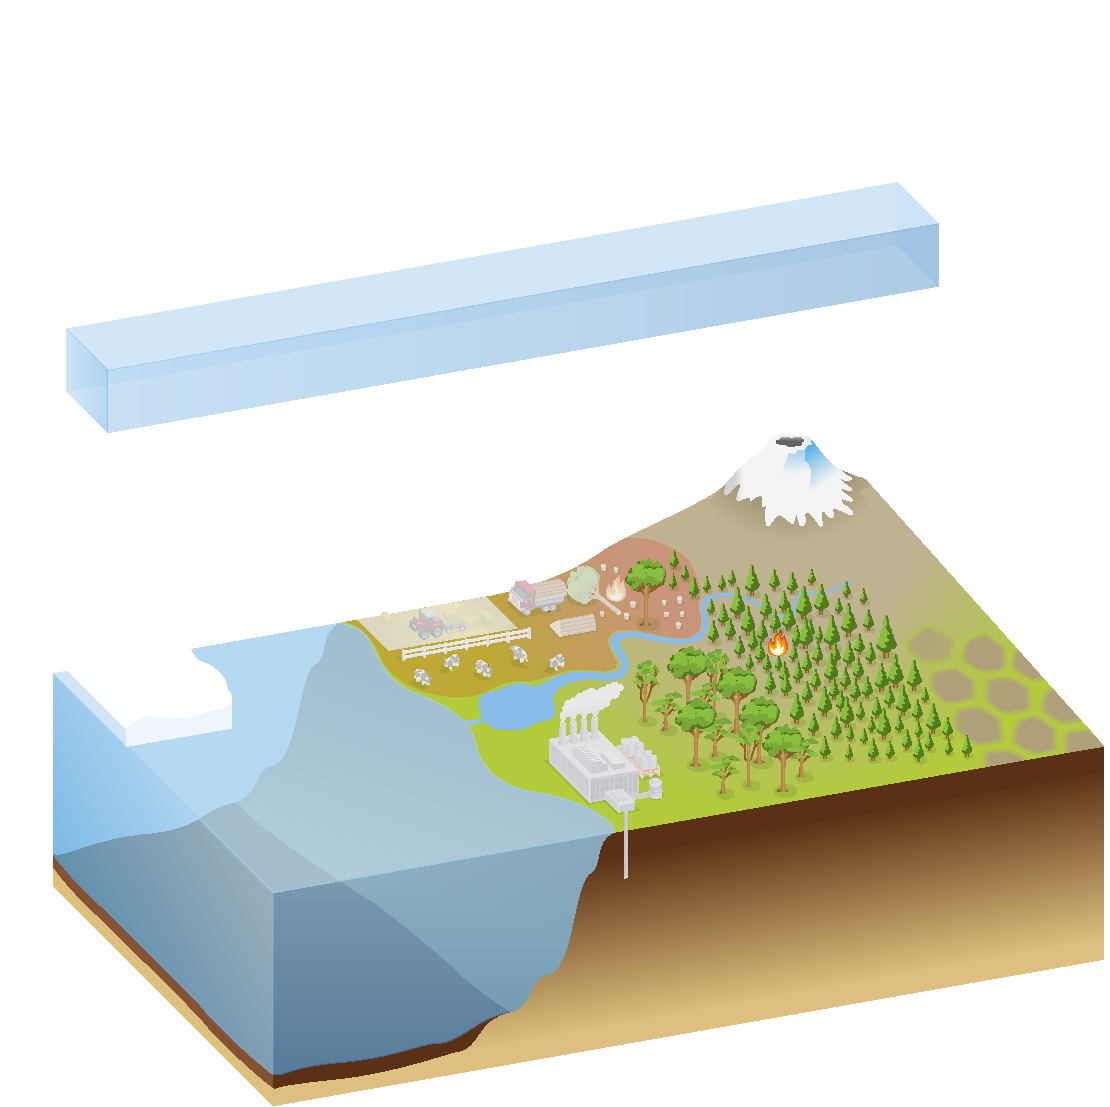
\includegraphics[trim={1cm 0cm 0cm 3cm}, clip, width=0.8\linewidth]{%
        bilder/climate_components/global_climate_components_spheres_ex_human.pdf}
	 	\caption{Schematische Abbildung des Klimasystems, Quelle: IPCC 2013, Physical Science Base, Kapitel 6} % Anmerkungen hinzugefügt nach
	\end{figure}
  \column{0.3\linewidth}
  \textbf{Sphären des Klimasystems}\\
  (altgriechisch)\\[1em]
  \textit{atmos} = Dunst\\
  \textit{hydor} = Wasser\\
  \textit{kryos} = Eis\\
  \textit{bios} = Leben\\
  \textit{pedon} = Boden\\
  \textit{lithos} = Stein
	%TODO: Evtl Bezeichnungen in Bild einfügen anstatt separat auflisten
	\end{columns}

	\note{
	\begin{itemize}
    \item[] Sphären
    \begin{itemize}
      \item[] Atmosphäre: Gasförmige Hülle der Erde\\
      \item[] Hydrosphäre: Ozeane, sowie Wasserkreislauf auf den Kontinenten
              und in der Atmosphäre\\
      \item[] Kryosphäre: Schnee und Eis\\
      \item[] Biosphäre: Lebewesen, Tiere und Pflanzen\\
      \item[] Pedosphäre: Boden\\
      \item[] Lithosphäre: Gestein
    \end{itemize}
		\item[] Hier: Vorstellung aller Sphären, sowie einiger wichtiger Interaktionen zwischen ihnen.
		\item[] Die Effekte des Klimawandels sind bereits heute spürbar: Dürreperioden und Überflutungen, Rückgang der Eisschilde und Waldrodung.
		\item[] Die Zustände der Böden sind entscheidend für die Vegetation und Landwirtschaft.
		\item[] $\rightarrow$ Erosion von Böden durch Übernutzung und Dürren macht sie unfruchtbar (Nährstoffverlust und Austrocknung).
		\item[] $\rightarrow$ Gestein liefert Mineralien, was ebenfalls für die Vegetation und auch z.B. Schalenbildung bei Muscheln wichtig ist.
	\end{itemize}
	}
\end{frame}

\begin{frame}
	\frametitle{Atmosphäre - Luftmassen}

	\begin{figure}
		\centering
		\begin{tikzpicture}
			\node (image1) {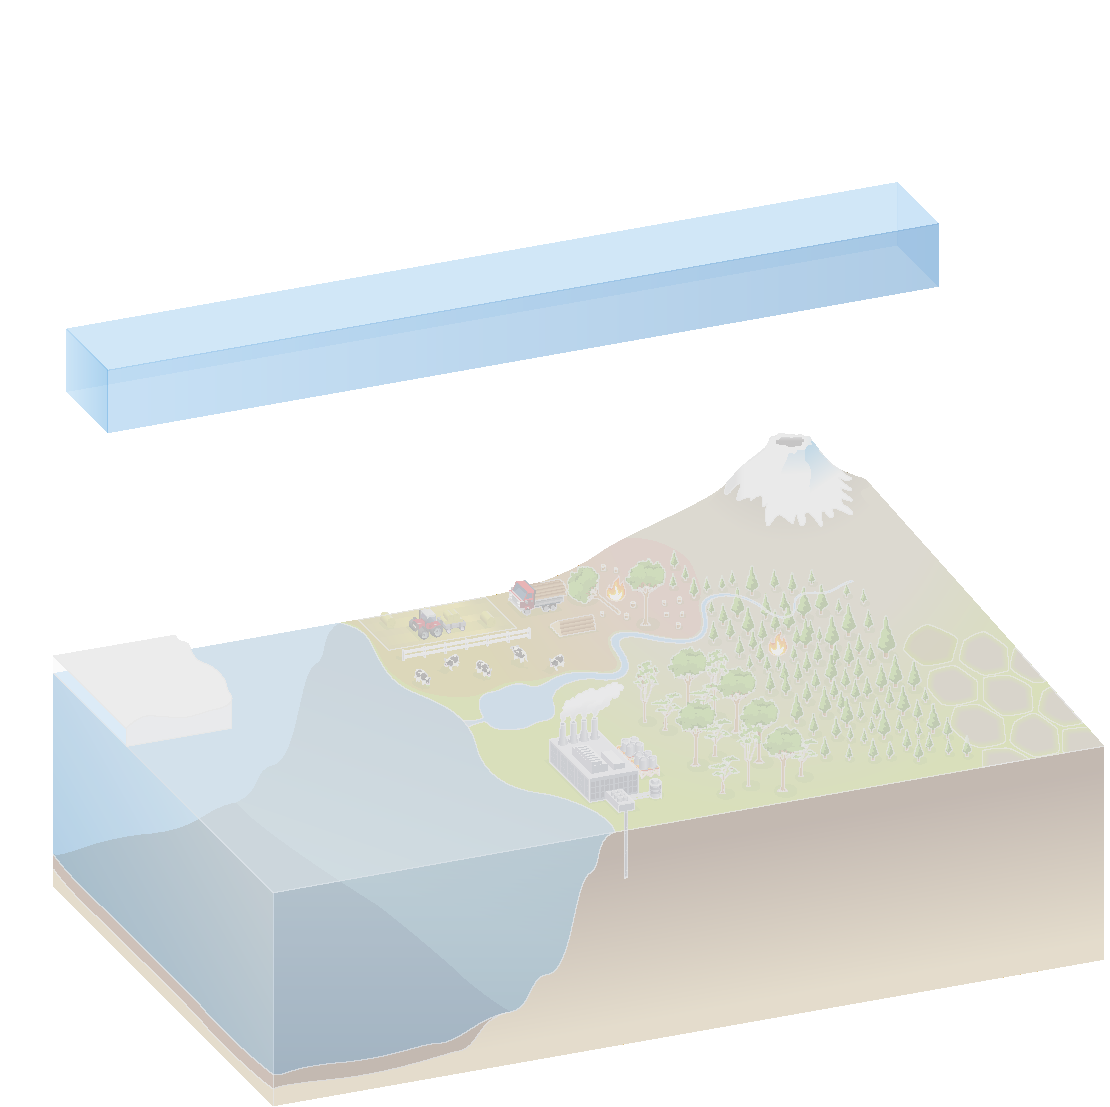
\includegraphics[trim={1cm 0cm 0cm 3cm}, clip, width=0.55\linewidth]{%
        	bilder/climate_components/global_climate_components_atmosphere.pdf}};
			\onslide<2|handout:0>\node (image2) at (image1.east) [xshift=-0.9cm]{%
					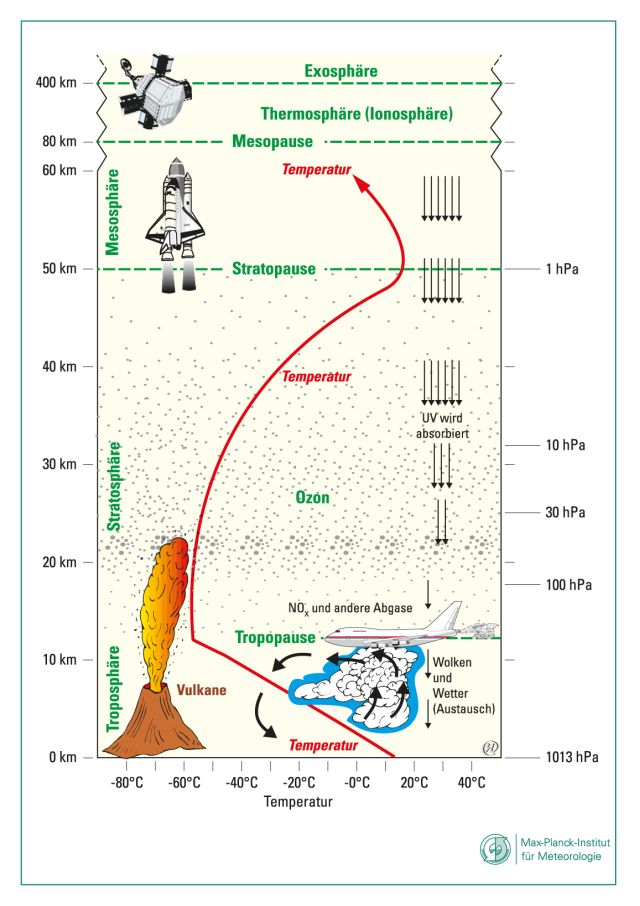
\includegraphics[width=0.35\linewidth] der Atmosphärenmasse, enthält fast allen Wasserdampf
			    \item[] Hier finden alle wetterrelevanten Phänomene statt
			  \end{itemize}
			  \item Stratosphäre, \SIrange{12}{50}{km}, \SIrange{-60}{0}{\celsius}, Ozon sorgt für Temperaturanstieg durch UV-Absorption
			  \item Mesosphäre, \SIrange{50}{80}{km}, \SIrange{-100}{0}{\celsius}, Temperatur fällt
			  \item Thermosphäre, \SIrange{80}{400}{km}, extrem geringe Teilchendichte, daher Temperatur nicht bestimmbar, Weltraum
			  \item Exosphäre, \SIrange{400}{1000}{km}, quasi Vakuum
			\end{itemize}
			\item[] Passt sich am schnellsten an Änderungen an $\rightarrow$ Wie funktionieren die Ausgleichsprozesse?
			\item[] in der planetaren Grenzschicht (\SIrange{1}{2.5}{km}): Reibung wichtig $\rightarrow$ starke vertikale Unterschiede in diesem Bereich der Atmosphäre
		\end{itemize}
		}
\end{frame}

\begin{frame}
	\frametitle{Globale Atmosphärische Zirkulation}

	\begin{figure}
		\centering
		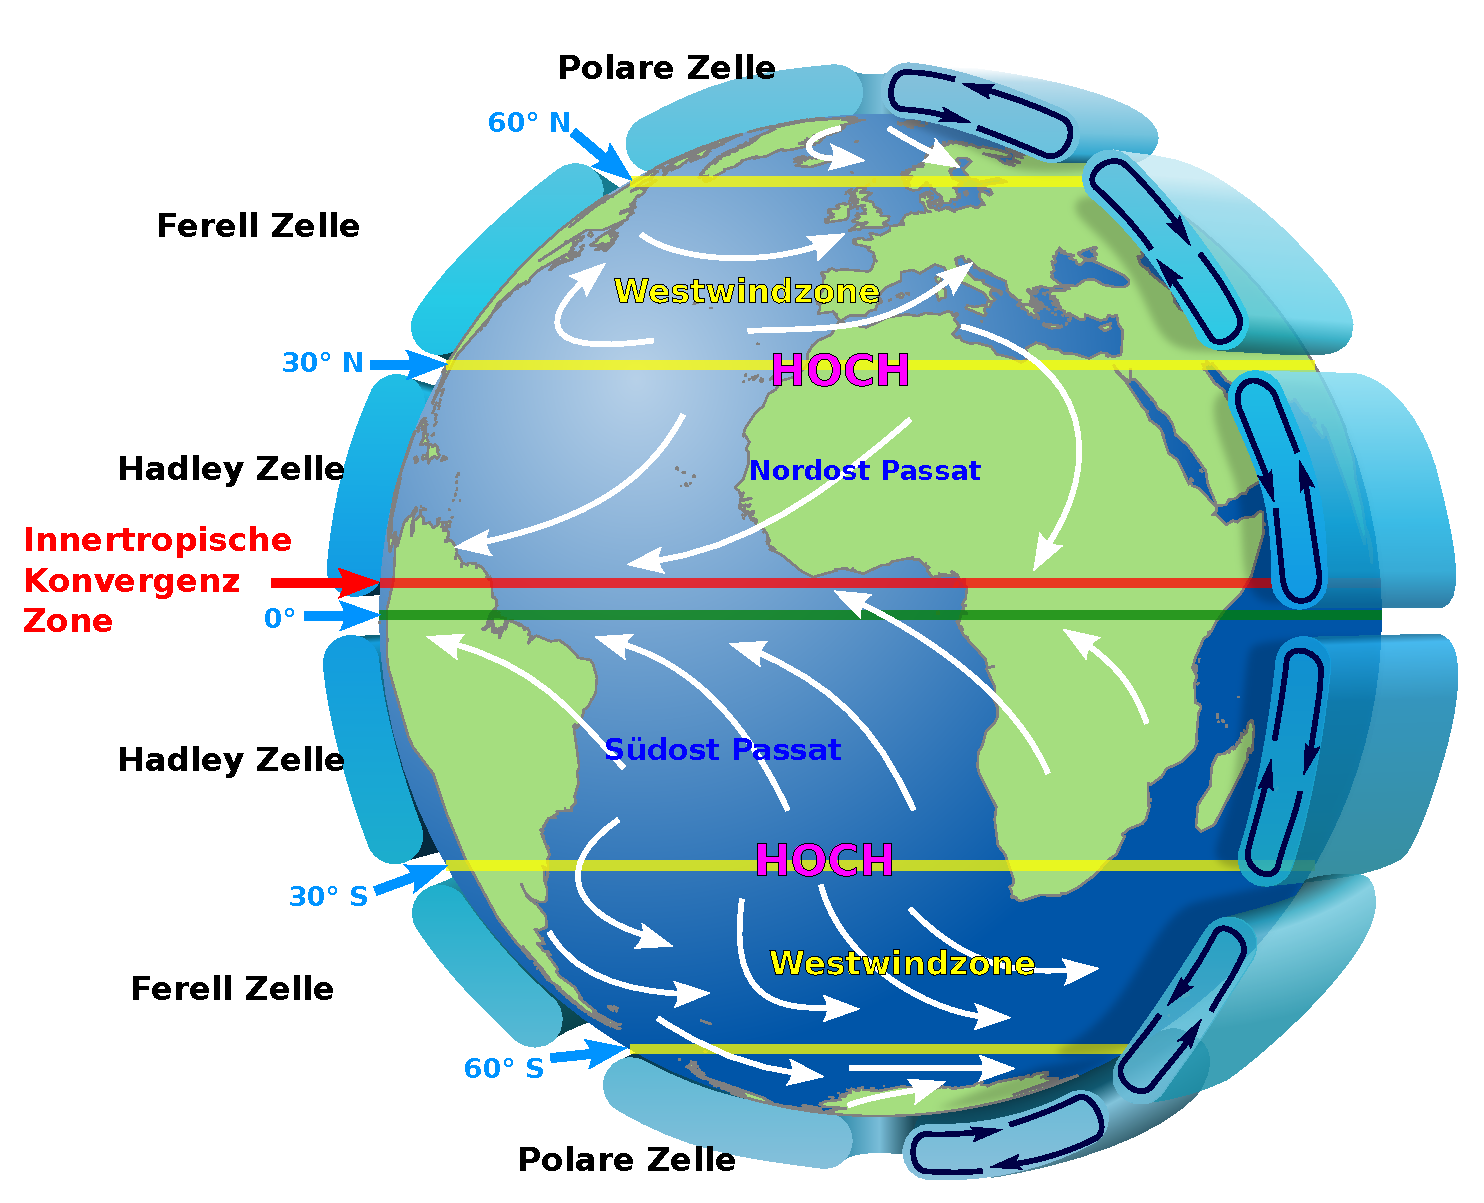
\includegraphics[width=.65\linewidth]{bilder/Earth_Global_Circulation_-_de.pdf}
		\caption{Globale atmosphärische Zirkulation, Quelle: MireRun/Kaidor nach NASA Global circulation of Earth's atmosphere}
	\end{figure}

	\note{
	Großskalige Modellvorstellung globaler Zirkulationssysteme in der Atmosphäre

	Starke Vereinfachung:
		\begin{itemize}
			\item[] Am Äquator steigt warme Luft auf, hinterlässt ein Tiefdruckgebiet (weniger Luft vorhanden).
    	\item[] In Bodennähe strömt kältere Luft in Richtung Äquator nach.
			\item[] Wegen der Drehung der Erde (Corioliskraft) werden Bewegungen auf der Nordhalbkugel im Uhrzeigersinn abgelenkt, auf der Südhalbkugel gegen den Uhrzeigersinn. Eine äquatorwärts strömende Luftmasse wird dadurch auf der Nordhalbkugel zum Nordostwind, auf der Südhalbkugel zum Südostwind.
			\item[] In der Höhe kommt es zu Ausgleichsströmungen: Luftmassen, die über dem Äquator aufgestiegen sind, strömen in der Höhe wieder polwärts. Am Pol in der Höhe eintreffende Luftmassen sinken dort ab.
		\end{itemize}

		Etwas genauer:
		\begin{itemize}
			\item[] vom Äquator weg strömende Luftmassen, sinken wegen der polwärtigen Flächenkonvergenz der Erde über rund \SI{30}{\degree} Breite wieder ab (Hadley Zelle, Passatwinde).
			\item[] vom Pol weg strömende Luftmassen, erwärmen sich, steigen ab rund \SI{60}{\degree} Breite wieder auf (Polare Zelle).
    	\item[] Zwischen beiden Systemen jeder Hemisphäre jeweils ein dritte, gegenläufige Zelle (Ferell Zelle, Westwinde).
    	\item[$\rightarrow$] Sowohl auf der Nord- als auch auf der Südhalbkugel jeweils drei (bodennahe) Windsysteme,
			\item[] Innertropische Konvergenzzone trennt Nord- und Südhalbkugel, Tiefdruckrinne
		\end{itemize}
		\begin{itemize}
			\item[Hadley Z.] Passatwinde sehr stabil, zur schnellen Überquerung der Ozeane genutzt
			\item[Polare Z.] Sehr stabil
			\item[Ferell Z.] instabil, gegenläufig zu polarer Zelle und Hadley Zelle. Enthält ca. \SI{38}{\percent} der Energieunterschiede zwischen Pol und Äquator.
		\end{itemize}
	}
\end{frame}

\begin{frame}
	\frametitle{Hydrosphäre - Wassermassen}
	\begin{figure}
		\centering
		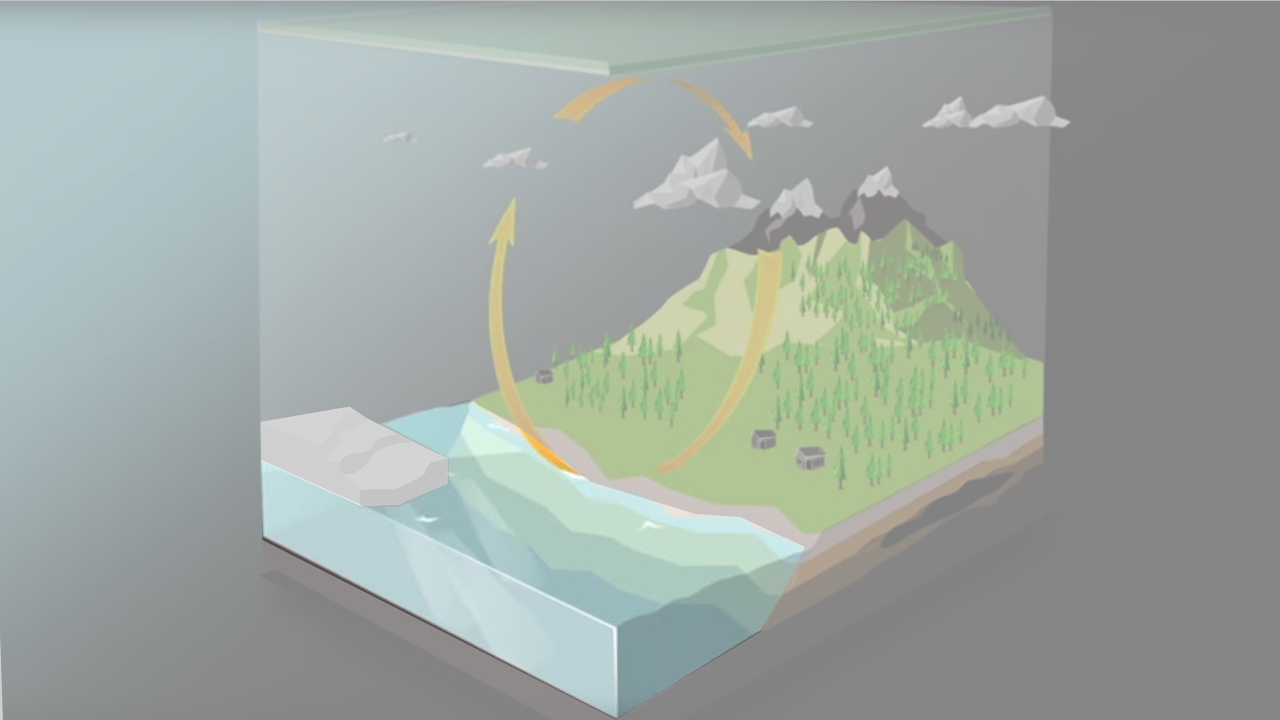
\includegraphics{bilder/WMO_Cycles_water.png}
		\caption{Etwa 2/3 der Erdoberfläche sind von Wasser bedeckt, somit ist die Hydrosphäre allein durch die Masse ein wichtiger Faktor des Klimasystems.}
	\end{figure}

	\note{
	\begin{itemize}
		\item[] Etwa 2/3 der Erdoberfläche sind von Wasser bedeckt, somit ist die Hydrosphäre allein durch die Masse ein wichtiger Faktor des Klimasystems.
		\item[] Daher widmen wir uns zuerst den Wassermassen.
		% Aufteilung von https://www.lenntech.de/faq-wasser-menge.htm, aber auch Wetzel, Robert G. 1983 in "Periphyton of freshwater ecosystems"
    \item[] Der Großteil der Wassermassen ist Salzwasser 97\,\%.
    \item[] Süßwasser (Flüsse und Seen) bildet nur weniger als 1\,\% des globalen Wassers.
    \item[] Eismassen machen ca. 2\,\% des Wassers aus und binden den größten Teil des Süßwassers, da das Salz bei der Eisbildung im Wasser gelößt bleibt.
    \item[] Eis betrachten wir später.
	\end{itemize}
	}
\end{frame}


\begin{frame}
	\frametitle{Eigenschaften des Wassers} % M.Latif Klimawandel und Klimadynamik S. 23
	\begin{itemize}
		\item Wasser ist ein Dipol-Molekül \textcolor{blue}{H$_2$O}
		\begin{itemize}
			\item[$\rightarrow$] Kann wirksam Infrarotstrahlung absorbieren
			\item[$\rightarrow$] Kann viel Wärme aufnehmen bevor es verdampft $\rightarrow$ "Trägheit"
		\end{itemize}

		%Allgemein liegt die größte Dichte des Wassers bei 4 Grad
		\item<2-> Größte Dichte von reinem Wasser bei \SI{4}{\degreeCelsius}
		\begin{itemize}
			\item<2->[$\rightarrow$] Eis schwimmt auf Wasser
		\end{itemize}
		% Im besonderen Fall des Salzwassers liegt die größte Dichte jedoch bei -3.8 Grad
		\item<3->Größte Dichte von Salzwasser bei \SI{-3,8}{\degreeCelsius}
		\begin{itemize}
			\item<3-> [] Bei der Eisbildung wird verbleibt das Salz gelößt im Wasser
			\item<3-> [$\rightarrow$] Wasser kann kälter werden als Eis und sinkt in die tieferen Schichten des Ozeans
			\item<3-> [$\rightarrow$] Wärmeres, weniger dichtes Wasser steigt auf
			\item<3-> [] \textbf{\textcolor{blue}{Konvektion}} in den Polarregionen
			\item<3-> [$\rightarrow$] Kohlenstoffsenken
		\end{itemize}
	\end{itemize}

	\note{
		\begin{itemize}
      \item[] erst die Slide vorstellen
			\item[] Das Phänomen Konvektion ist nicht auf Wasser beschränkt. Gibt es auch in der Luft oder wird durch Pumpen erzeugt.
			\item[] die Konvektion ist durch die temperaturbedingte Dichte und den Salzgehalt möglich
			\item[] daher auch unter dem Namen \textit{thermohaline Konvektion} (thermo - Temperatur, halin - Salz) bekannt
		\end{itemize}
	}

% TODO: evtl. Abbildung der Konvektion: Abgabe von Wärme bei Aufnahme von atmosphärischen Gasen, die dann in die Tiefsee gelangen und dort gespeichert werden

%TODO: Erklärung von Senken
\end{frame}

\begin{frame}
	\frametitle{Wasserdynamik} %M. Latif Klimawandel und Klimadynamik S.24
	\begin{figure}
    \centering
    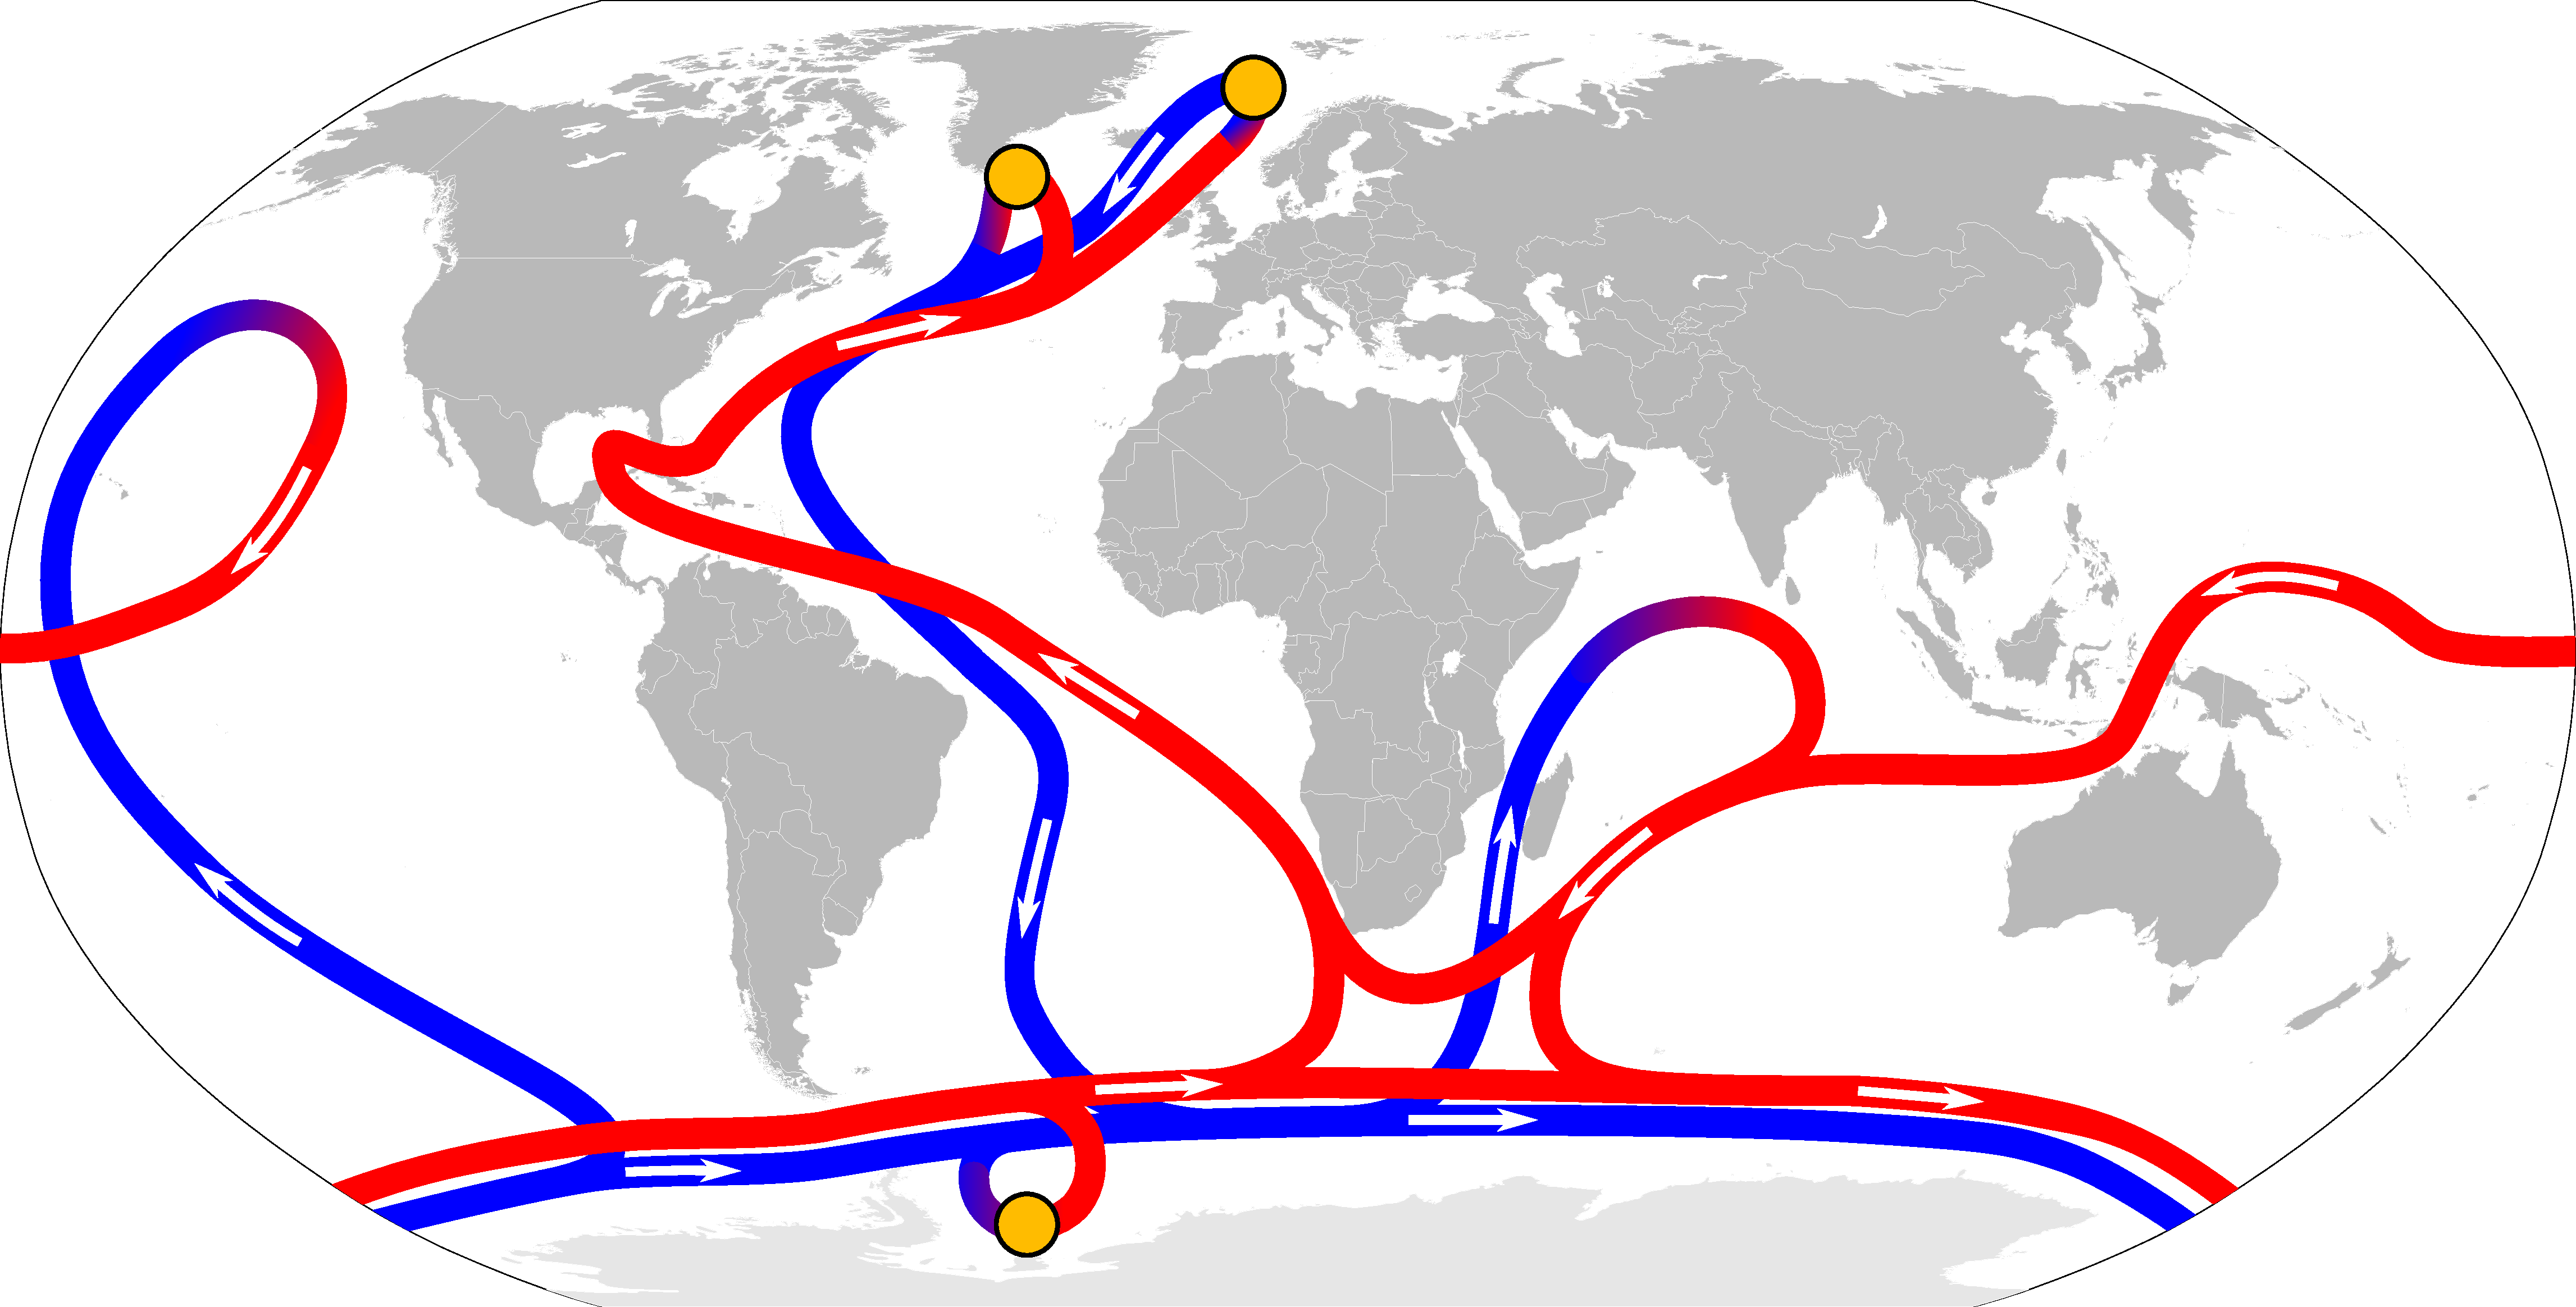
\includegraphics[width=.9\linewidth]{bilder/Thermohaline_Circulation.pdf}
    \caption{Termohaline Zirkulation, Quelle: nach Robert Simmon, NASA}
  \end{figure}

	\note{
		\begin{itemize}
			\item[] Die großen Wassermassen der Ozeane haben eine bestimmte Strömung, z.B. Golfstrom von der Arktis über die Küste Mexikos bis an die Antarktis.
			\item[] Die Stömung ergibt sich vorallem durch die Erdrotation (Corioliskraft).
			\item[] Die oberflächliche Strömung der oberen 100 Meter entsteht durch Wind (und darauf resultierende Reibung) und die Form der Meeresbecken.
			\item[] Die Tiefenströmung wird durch die Konvektion angetrieben. Die Dichte des Wassers spielt dabei eine entschiedende Rolle, da dichteres Wasser nach unten sinkt und leichteres empor steigt.
			\item[] Warme Temperaturen führen zum aufwärmen des Oberflächenwassers und damit zu einer geringeren Dichte.
			\item[] Dadurch werden Oberflächenwasser und Tiefenwasser stark getrennt - und somit strömen die Wassermassen mit unterschiedlicher Geschwindigkeit.
      \item[] Unterscheidung zwischen zwei Zirkulationen
      \begin{itemize}
        \item[Windgetrieben] Oberflächenströmung der Ozeane durch Reibung, Erdrotation (Corioliskraft) und Form der Meeresbecken, eher horizontal
        \item[Dichtegetrieben] Erwärmung, Abkühlung, und Änderung des Salzgehaltes (durch Eisbildung, Verdunstung oder Niederschlag) haben Einfluss auf die Dichte des Wassers, wodurch die Wassermassen zirkulieren, eher vertikal
      \end{itemize}
		\end{itemize}
	}

\end{frame}


\begin{frame}
	\frametitle{Wirkung des Wassers auf das Klima}
	\begin{itemize}
	\item Ca. 70\,\% der Erdoberfläche ist mit Wasser bedeckt
	\item [$\rightarrow$] Die \textit{Trägheit} des Wassers ist ein entscheidender Faktor für die Trägheit des Klimas und der Klimaänderungen % M.Latif Klimawandel und Klimadynamik S. 23
	\item Kohlenstoffsenken in der Tiefsee können durch erwärmen der Ozeane \textit{irgendwann} freigesetzt werden
	\item[$\rightarrow$] massiver Anstieg des atmosphärischen CO$_2$ $\rightarrow$ Verstärkung des Treibhauseffekts
	\item Positive Verstärkung von CO$_2$ und Wasserdampf: eine wärmere Atmosphäre kann mehr Wasserdampf (und CO$_2$) aufnehmen
	\end{itemize}
\end{frame}

\begin{frame}
	\frametitle{Trägheit des Klimas}
	\begin{figure}
		\centering
		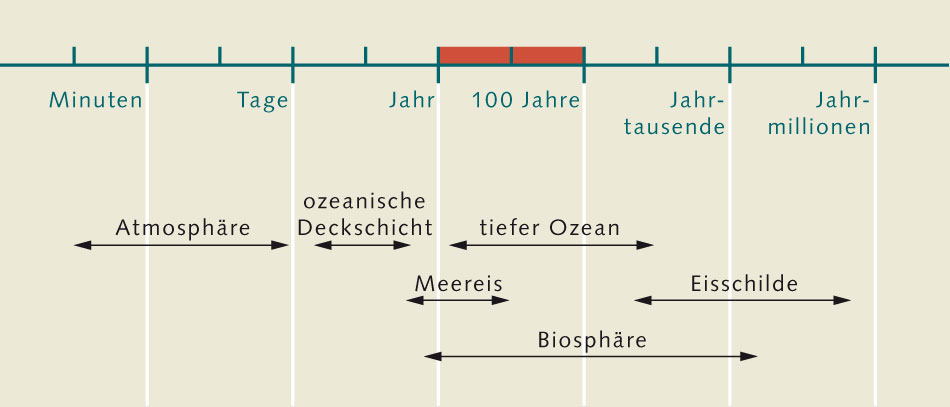
\includegraphics[width=0.8\linewidth]{bilder/zeitskala-klimasystem_world_ocean_review.jpg}
		\caption{Zeitskalen im Klimasystem, Quelle: maribus nach Meinecke und Latif, 1995}
		\label{fig:traegheit}
	\end{figure}

  \begin{itemize}
    \item[$\rightarrow$] Verzögertes Feedback bis zu einem klimawirksamen Ereignis.
    \item[$\rightarrow$] Besonders die Ozeane und Eisschilde benötigen eine sehr lange Zeit, um sich geänderten klimatischen Bedingungen anzupassen.
  \end{itemize}

	\note{
		\begin{itemize}
			\item[] Trägheit des Wassers ist entscheident.
			\item[] Die Wassermassen sind in dieser Abbildung stark vertreten.
			\item[] Die untere Atmosphäre passt sich innerhalb weniger Stunden den Bedingungen der Erdoberfläche an (Temeperatur, Gase, etc.)
			\item[] Die Wassermassen reagieren sehr unterschiedlich.
			\item[] Flüsse, Seen und Oberflächenwasser wärmen sich dabei deutlich schneller auf als die tieferen Ozeanschichten. (Das kennt man vielleicht aus Bade- oder Bergseen - die oberen 50 cm sind angenehm warm und darunter liegt deutlich kälteres Wasser)
			\item[] Besonders unterschiedlich schnell reagiert die Biosphäre.
      \begin{itemize}
        \item[] Graslandschaften können schnell austrocken
        \item[] Wälder dagegen verändern sich über Jahrtausende hinweg.
        \item[] Die Vegetation bestimmt in vielen Fällen auch die Ansiedlung von Lebewesen.
        \item[] Die Änderung der Vegetation kann das Ende des Lebenraums einiger Lebewesen bedeuten, aber auch neue Ansiedluneg bedingen.
      \end{itemize}
			\item[] Eine besonders lange Reaktionszeit haben die Eisschilde der Erde. Auf die Eismassen gehen wir als nächstes ein.
		\end{itemize}
	}
\end{frame}

\begin{frame}
	\frametitle{Kryosphäre - Eismassen}

	\begin{figure}
		\centering
		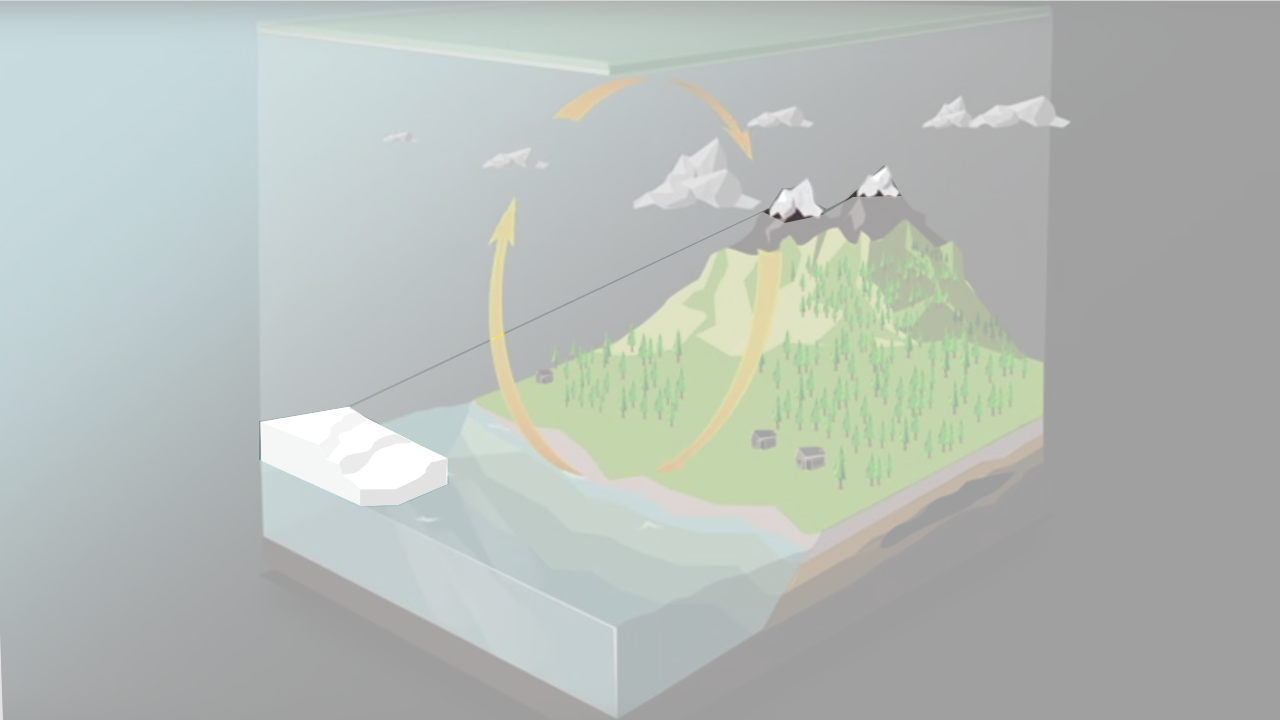
\includegraphics{bilder/WMO_Cycles_ice.png}
		\caption{Kryosphäre umfasst alle Formen und Schnee und Eis}
	\end{figure}
	\note{
		\begin{itemize}
			\item[] Eismassen stellen nach den Ozeanen die zweitgrößte Komponente des Klimasystems dar.
			\item[] das liegt an der Wärmekapazität von Wasser und seinem Volumen
      \begin{itemize}
        \item[] Wasser: \SI{4,18}{kJ \per kg \per K} bei \SI{20}{°C}
        \item[] Gestein etwa: \SIrange{0,7}{1}{kJ \per kg \per K}
      \end{itemize}
      \item[] ca. 2\,\% des Wassers ist in fester Form in Gletschern und an den Polkappen dauerhaft gebunden.
  %		\item  inländische Eisflächen speichern ca. 75\% des globalen Süßwassers
  		\item[] Eis reflektiert die ankommende Sonnenstrahlung zu großen Teilen
  		$\rightarrow$ \textbf{\textcolor{blue}{Albedo-Effekt}}\\

  		\item[] Je weniger Eismassen, desto weniger Strahlung wird reflektiert und bleibt in der Atmosphäre $\rightarrow$ Verstärkung des Treibhauseffekts

  		\item[] Durch Rußablagerungen auf den Eismassen wird mehr Sonnenstrahlung absorbiert ("Black Carbon")
  		 $\rightarrow$ Schmelzen des Eis und Verringerung des Albedo-Effekts % (Nature Geoscience, 2014; doi: 10.1038/ngeo2180)
		\end{itemize}
	}
\end{frame}


\begin{frame}
	\frametitle{Kryosphäre - Komponenten}
	Die größten Komponenten der Kryosphäre sind:
	\begin{itemize}
		\item Meereis: schwimmende Eismassen, 19-27 Mio. km$^2$
		\item Eisschilde: über Grönland und der Antarktis, 14 Mio. km$^2$
		\item Permafrost: gefrorene Böden, 22,8 Mio. km$^2$
	\end{itemize}

	\glqq Ein einmal eingesetzter Rückzug großer kontinentaler Eisschilde kann selbst nach Stabilisierung der Randbedingungen [(CO$_2$-Emissionen)] über ein Jahrtausend lang anhalten\grqq{} (Latif, 2009 und IPCC, 2001)\\
	%$\rightarrow$ siehe auch: Trägheit des Klimas in Abbildung \ref{fig:traegheit}

	\note{
		\begin{itemize}
			\item[] Meereis flächenmäßig sehr groß, aber Volumen der Eisschilde deutlich größer
			\item[] Eisschilde durchschnittlich 1,7-2 km dick
			\item[] weitere Elemente:
			\item[] Schneebedeckung variiert jahreszeitlich besingt zwischen 2 und 45 Mio. km$^2$
			\item[] Gletscher bilden 'nur' 0.5 Mio. km$^2$
		\end{itemize}
	}
\end{frame}

\begin{frame}
	\frametitle{Meereis} % Bild -> Pexels Andrea Schettino
  \begin{columns}
    \column{.3\linewidth}
    \begin{figure}
      \centering
      \newlength{\imagewidth}
      \settowidth{\imagewidth}{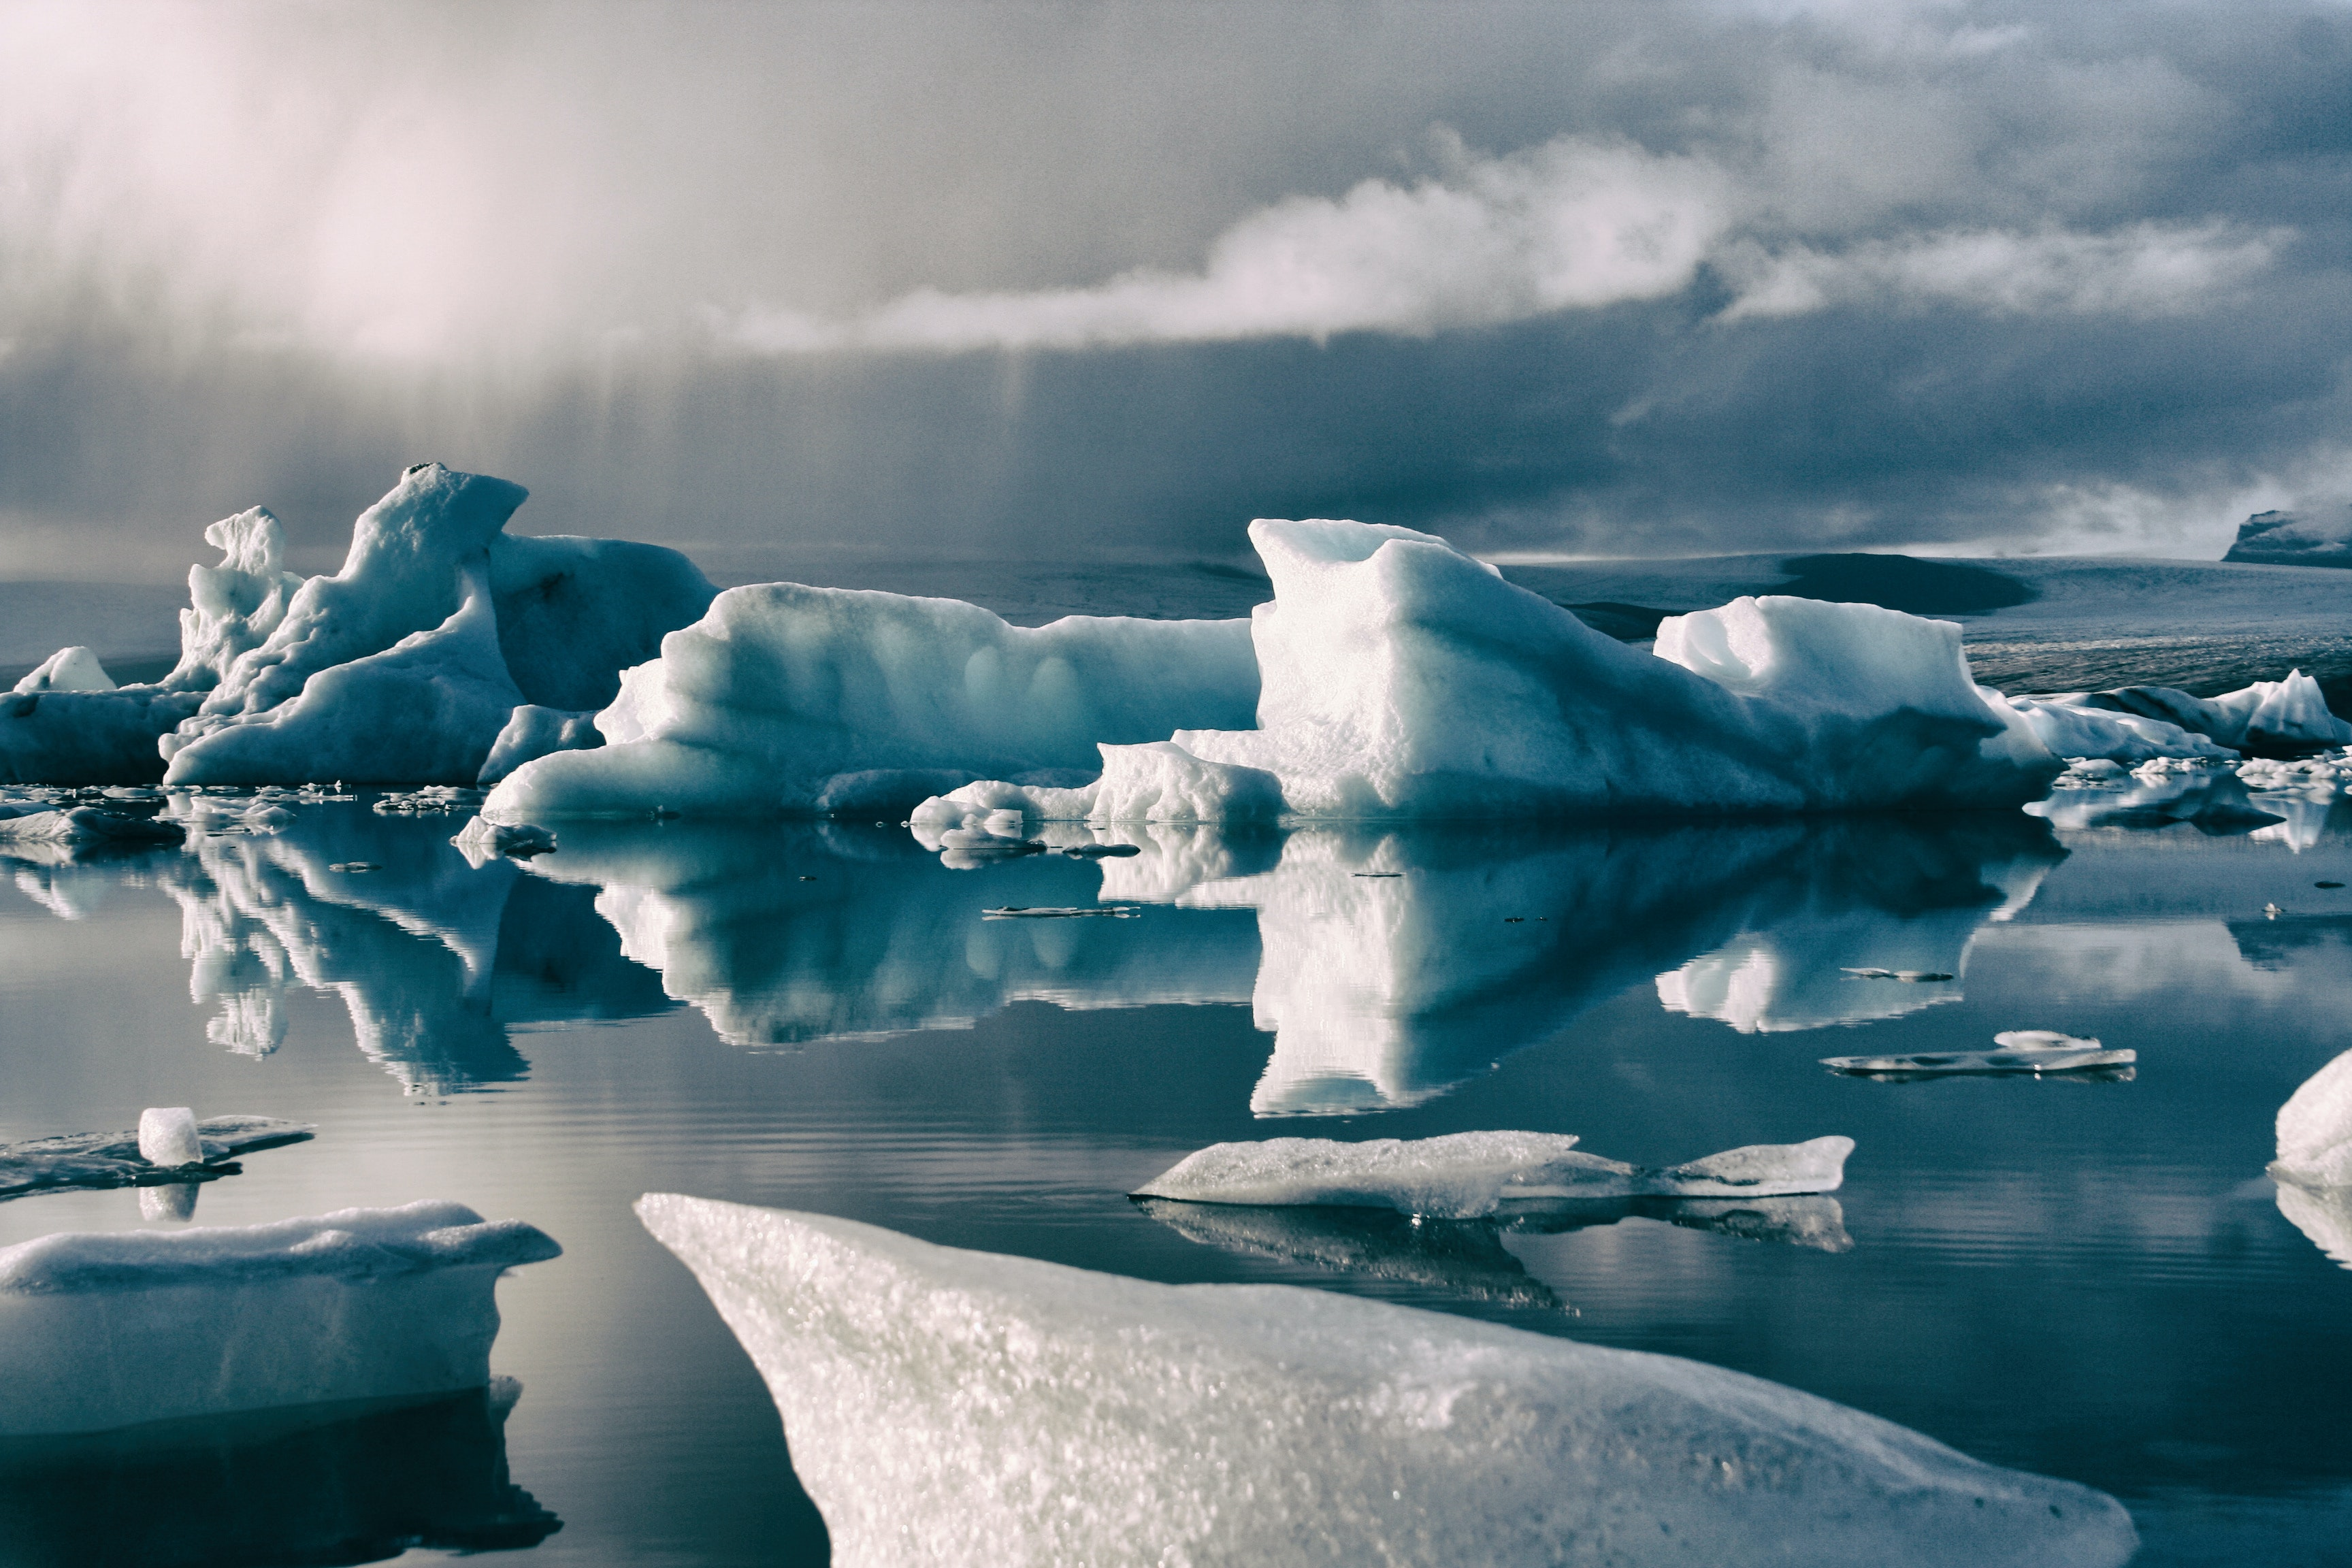
\includegraphics{bilder/ice-formation-in-body-of-water-3923277.jpg}}
      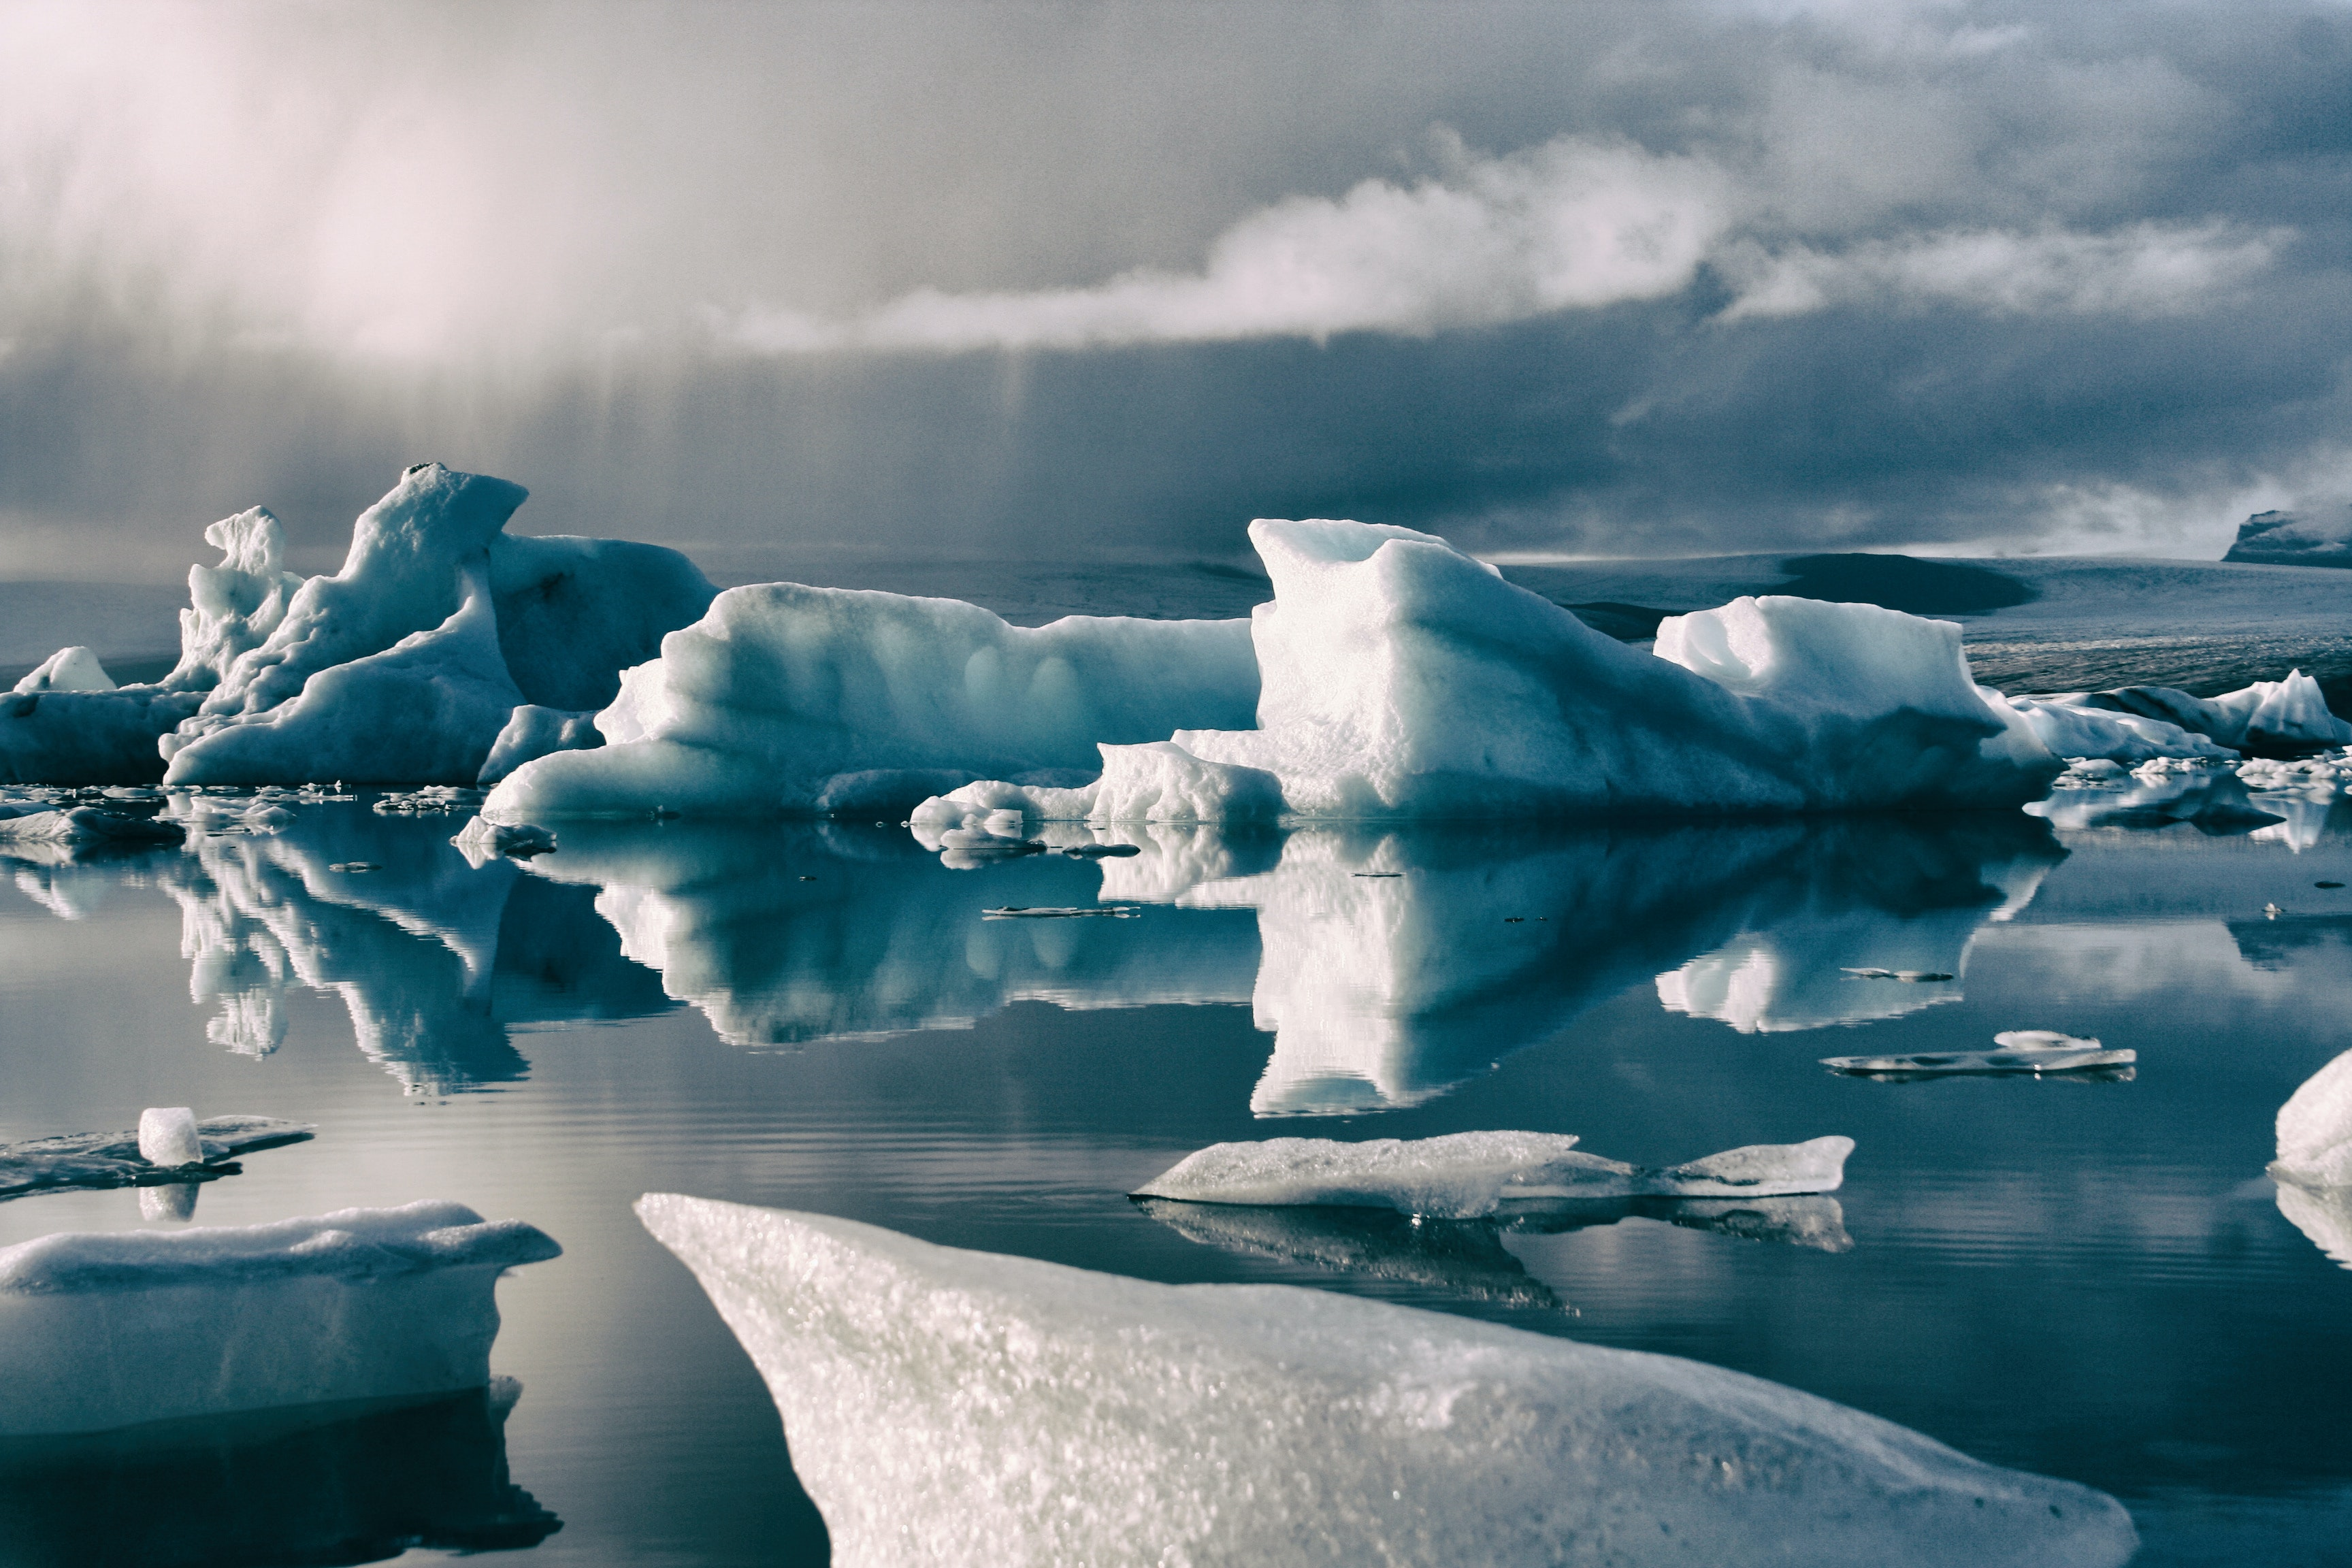
\includegraphics[trim=0 0 0.69\imagewidth{} 0, clip, width = 0.8\linewidth]{bilder/ice-formation-in-body-of-water-3923277.jpg}
      \caption{Quelle: Pexels, Andrea Schettino}
    \end{figure}
    \column{.7\linewidth}
	    \begin{itemize}
		    \item Bildet die Grenze zwischen Ozeanen und Atmosphäre
		    \item Luft über dem Meereis ist deutlich kälter als über dem Ozean
		    \item [$\rightarrow$] Abkühlung der Polarregionen und Verstärkung der atmosphärischen Zirkulation (Winde)
		    \item [$\rightarrow$] Beeinflusst Konvektion: je weniger Eis, desto schwächer die Konvektion, desto schwächer sind (langfristig) ozeanische Strömungen
	   \end{itemize}
   \end{columns}

	\note{
		\begin{itemize}
			\item[] Winde entstehen zum Dichte-/Wärmeausgleich, stärkere Tmeperaturunterschiede führen also zu stärkeren Winden
			\item[] Konvektion beeinflusst vorallem die Tiefseestömungen
			\item[] Weniger Konvektion bedeutet auch weniger Nährstoffe in oberen Schichten der Ozeane
		\end{itemize}
	}
\end{frame}

\begin{frame}
	\frametitle{Eisschilde}
  \begin{columns}
    \column{.3\linewidth}
    \begin{figure}
      \centering
      \settowidth{\imagewidth}{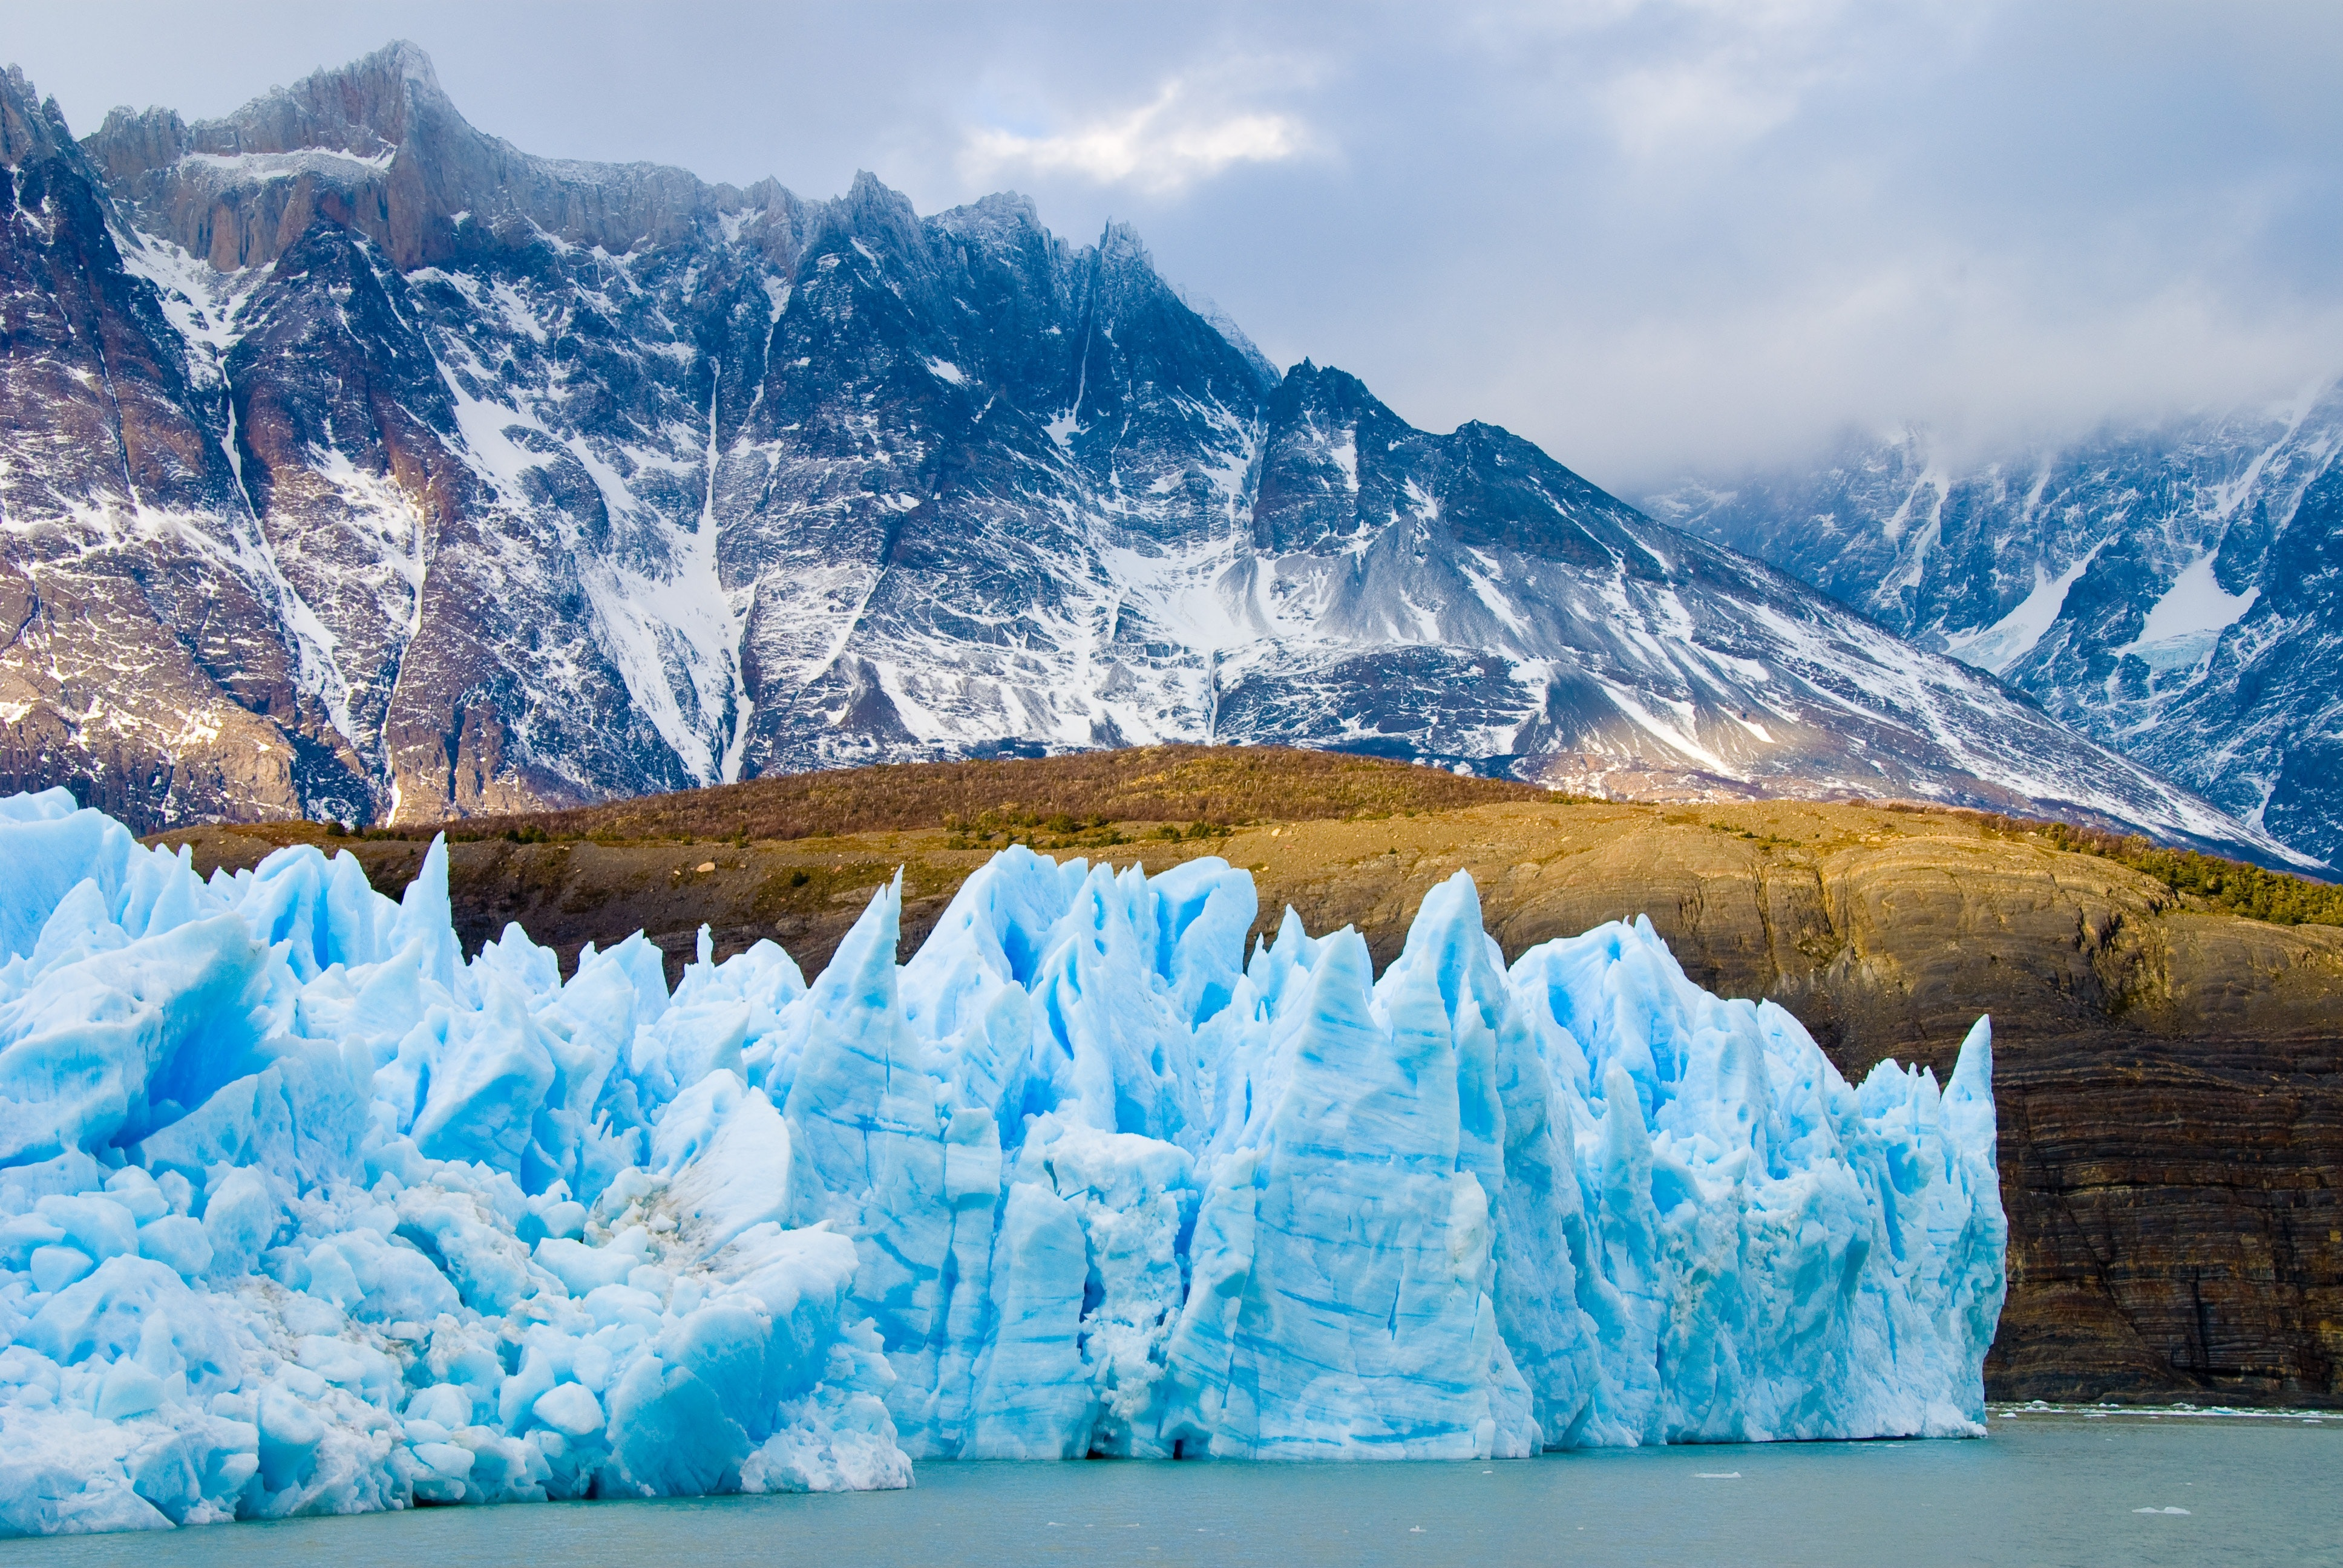
\includegraphics{bilder/panoramic-view-of-landscape-against-sky-255329.jpg}}
      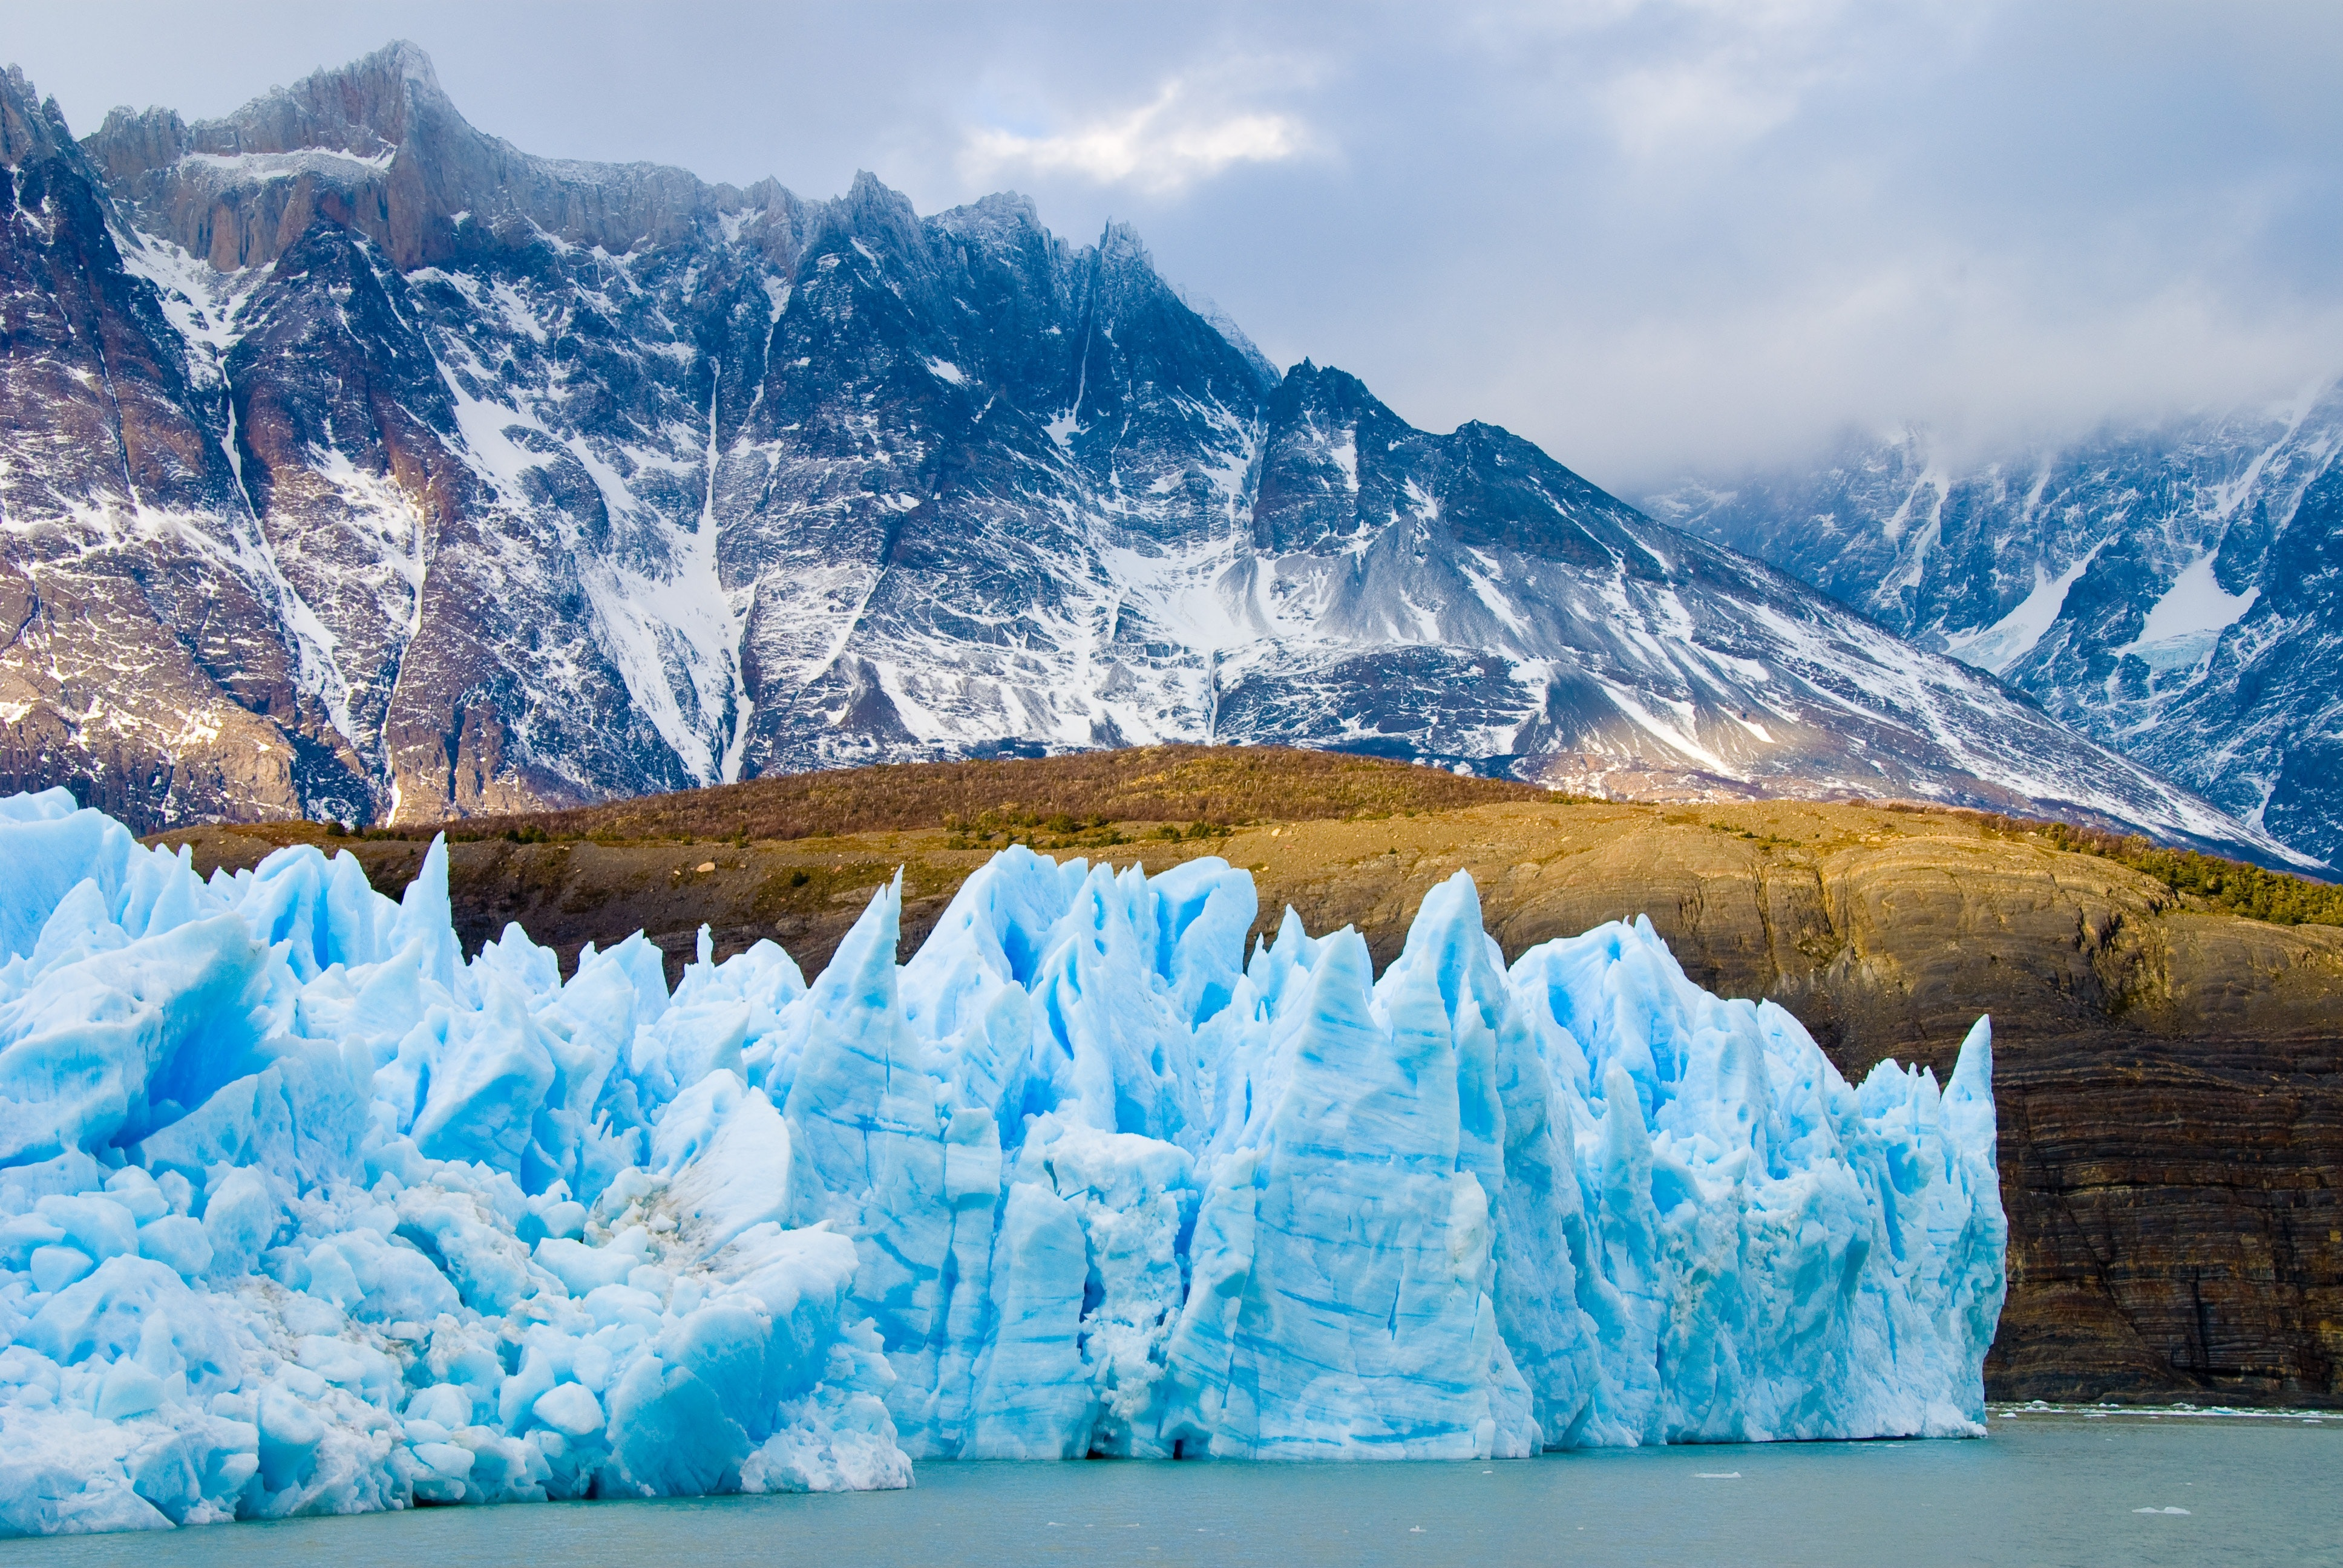
\includegraphics[trim=0 0 0.69\imagewidth{} 0, clip, width = 0.8\linewidth]{bilder/panoramic-view-of-landscape-against-sky-255329.jpg}
      \caption{Quelle: Pexels, Pixabay}
    \end{figure}
    \column{.7\linewidth}
	\begin{itemize}
		\item Volumen: 25 Mio. km$^3$ (Antarktis) + 3 Mio. km$^3$ (Grönland)
		\item Masse ist durch Niederschlag, Lufttemperatur und Strahlung bestimmt
		\item In der Antarktis gibt es Ausläufer des Landeises auf den Ozean hinaus (Schelfeis) $\rightarrow$ 0,7 Mio. km$^3$
%		\item tiefer liegende Schichten der Eisschilde schmelzen durch den Druck auf die Landmassen $\rightarrow$ erzeugt Spannungen im Eis
		\item Eisschilde schmelzen an randnahen Bereichen
		\item Höhere Temperaturen im Nordhalbkugelsommer gefährden das grönländische Eisschild besonders stark
		\item \textbf{Eisschilde haben das größte Potential für einen Anstieg des Meeresspiegels, da sie nicht -- wie das Meereis -- zum Meeresspiegel beitragen}
	\end{itemize}
  \end{columns}

	\note{
		\begin{itemize}
			\item[] Je mehr Schnee und je kälter, desto mehr Eis kann dich bilden
			\item[] Schelfeis zählt nicht zum Meereis, da es fest mit den Eisschilden verbunden ist
			\item[] Schelfeis bildet sich v.a. in Buchten, die von Eisschild umgeben sind
			\item[] Grönland besitzt quasi kein Schelfeis, daher schmilzt in Grönland direkt das Eisschild
			\item[] Der Antarktische Eisschild ist durch das Schelfeis etwas mehr geschützt
			\item[] Ein komplettes Abtauen der Eisschilde kann den Meeresspiegel bis zu 64 Meter ansteigen lassen. $\rightarrow$ sog. Meeresspiegel-äquivalent nach IPCC 2007
		\end{itemize}
	}
\end{frame}

\begin{frame}
	\frametitle{Permafrost}
  \begin{columns}
    \column{.3\linewidth}
    \begin{figure}
      \centering
      \settowidth{\imagewidth}{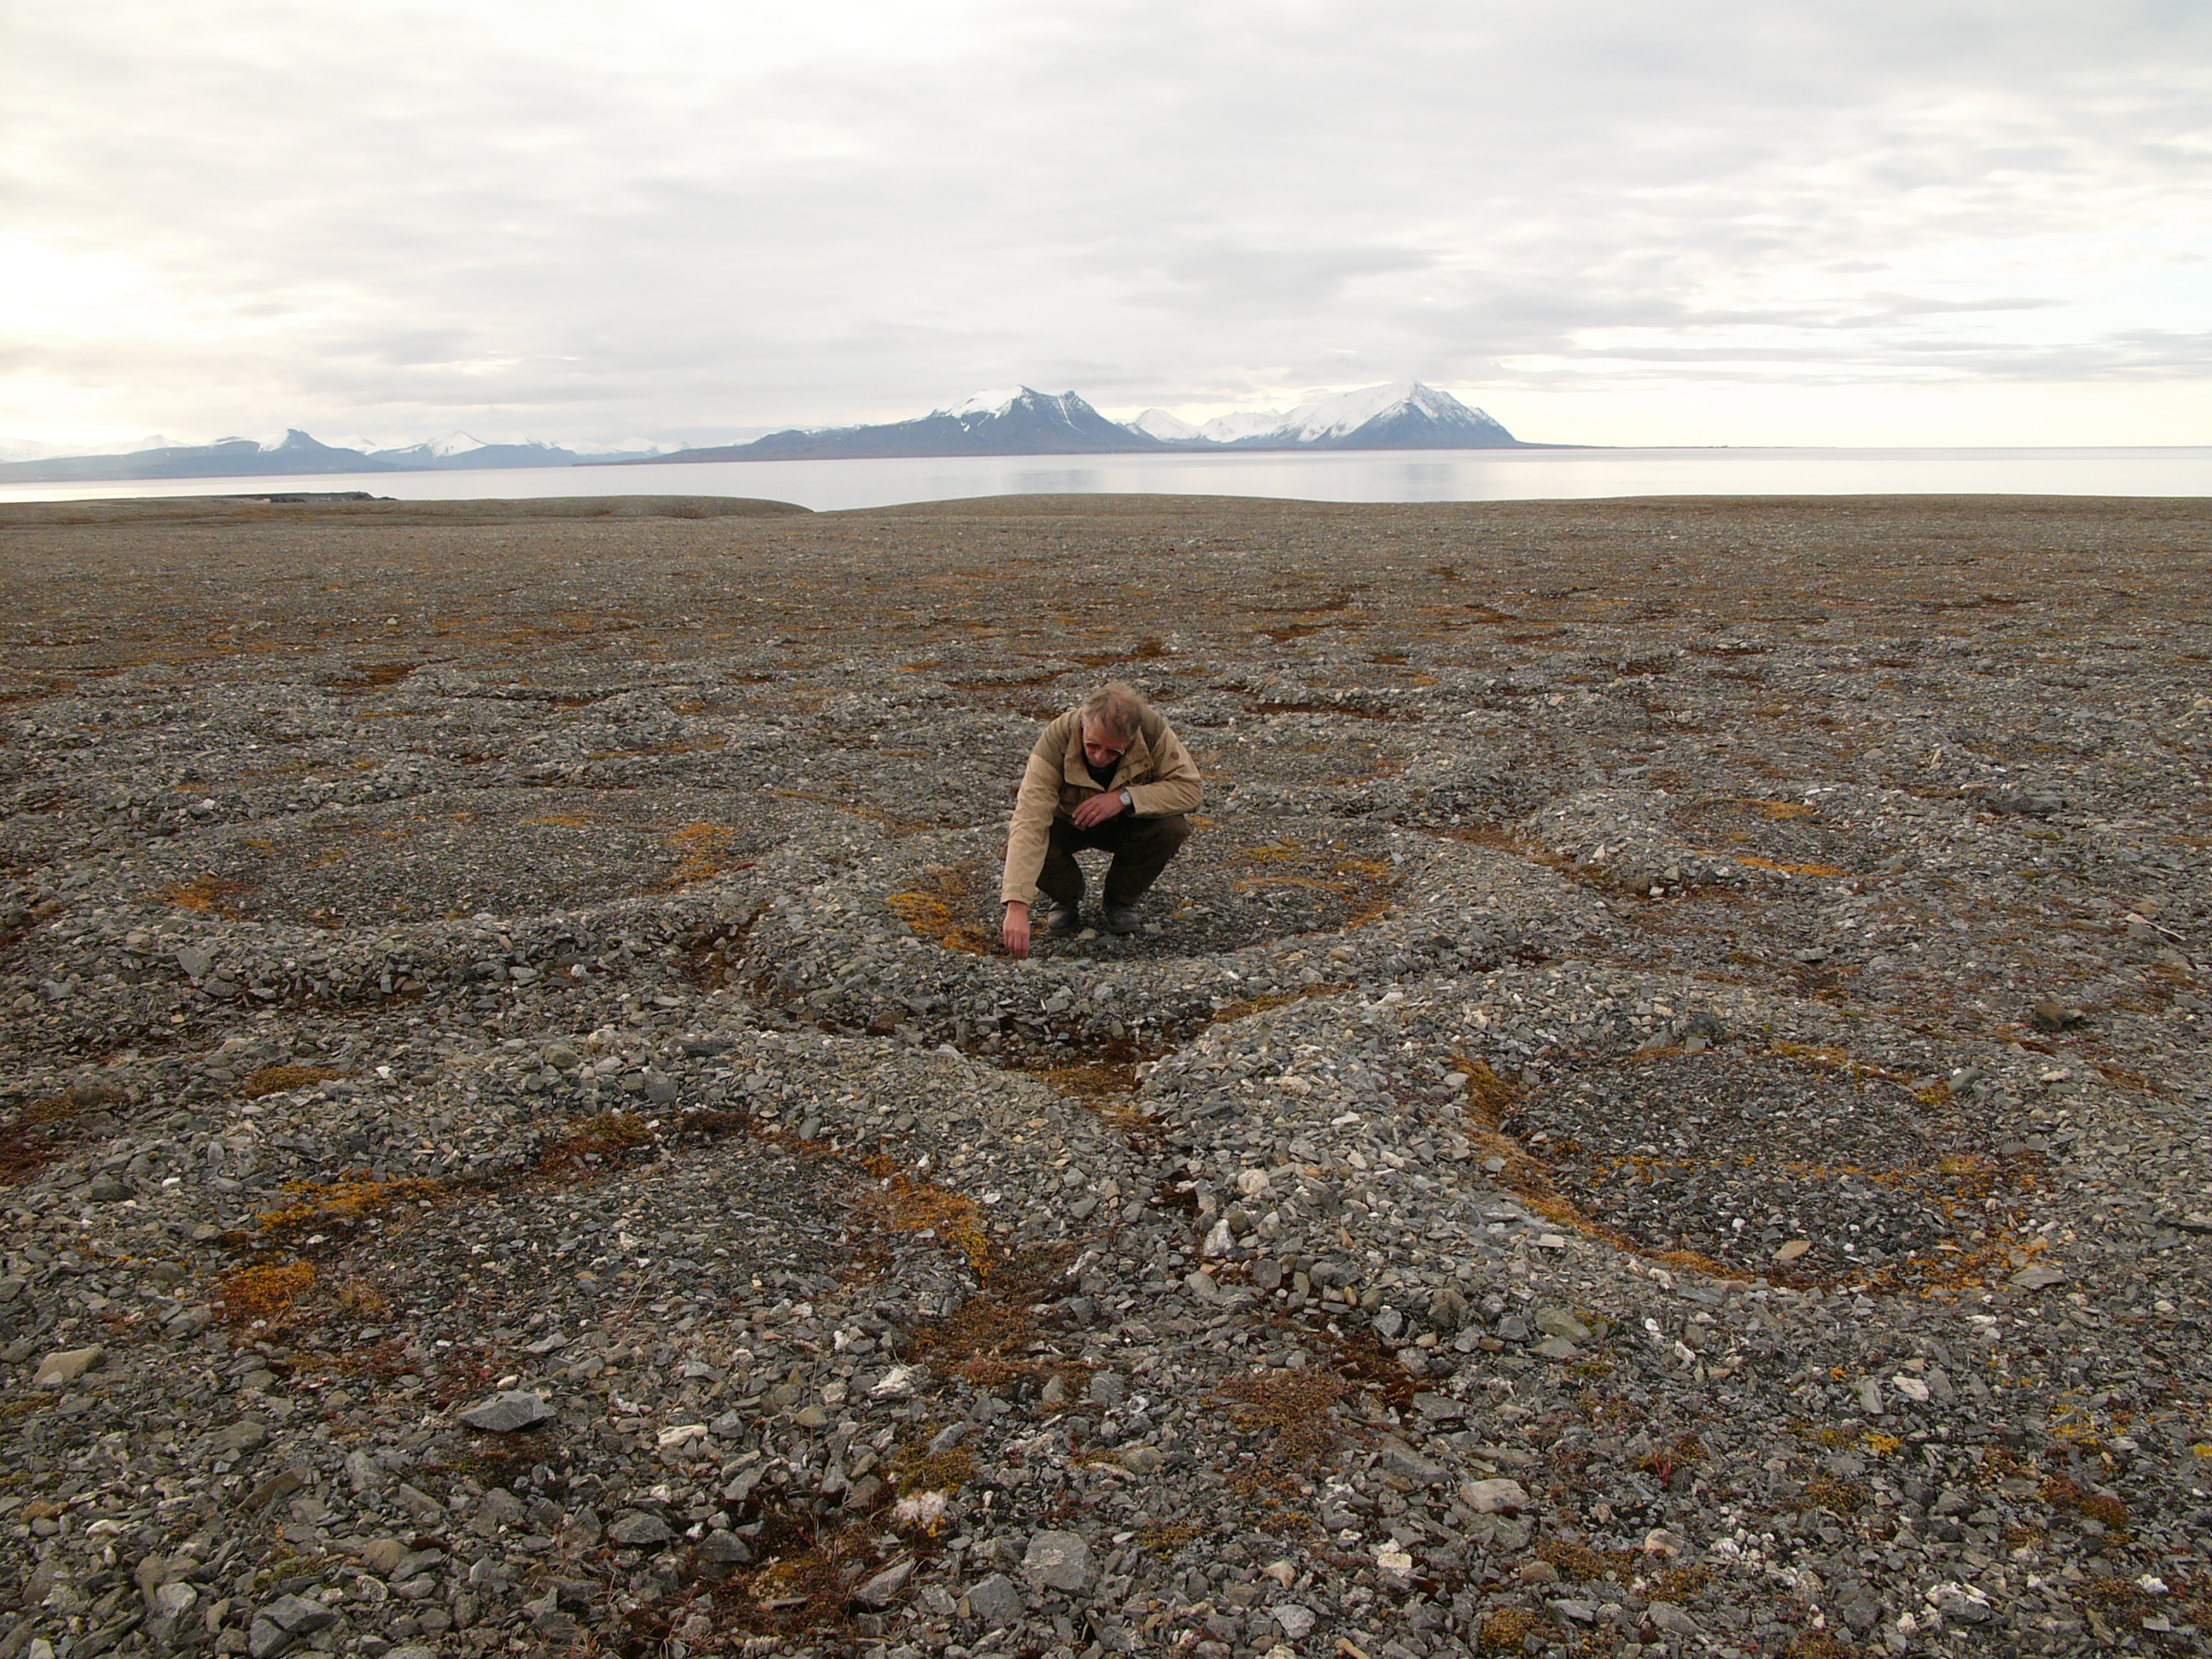
\includegraphics{bilder/Permafrost_stone-rings_hg.jpg}}
      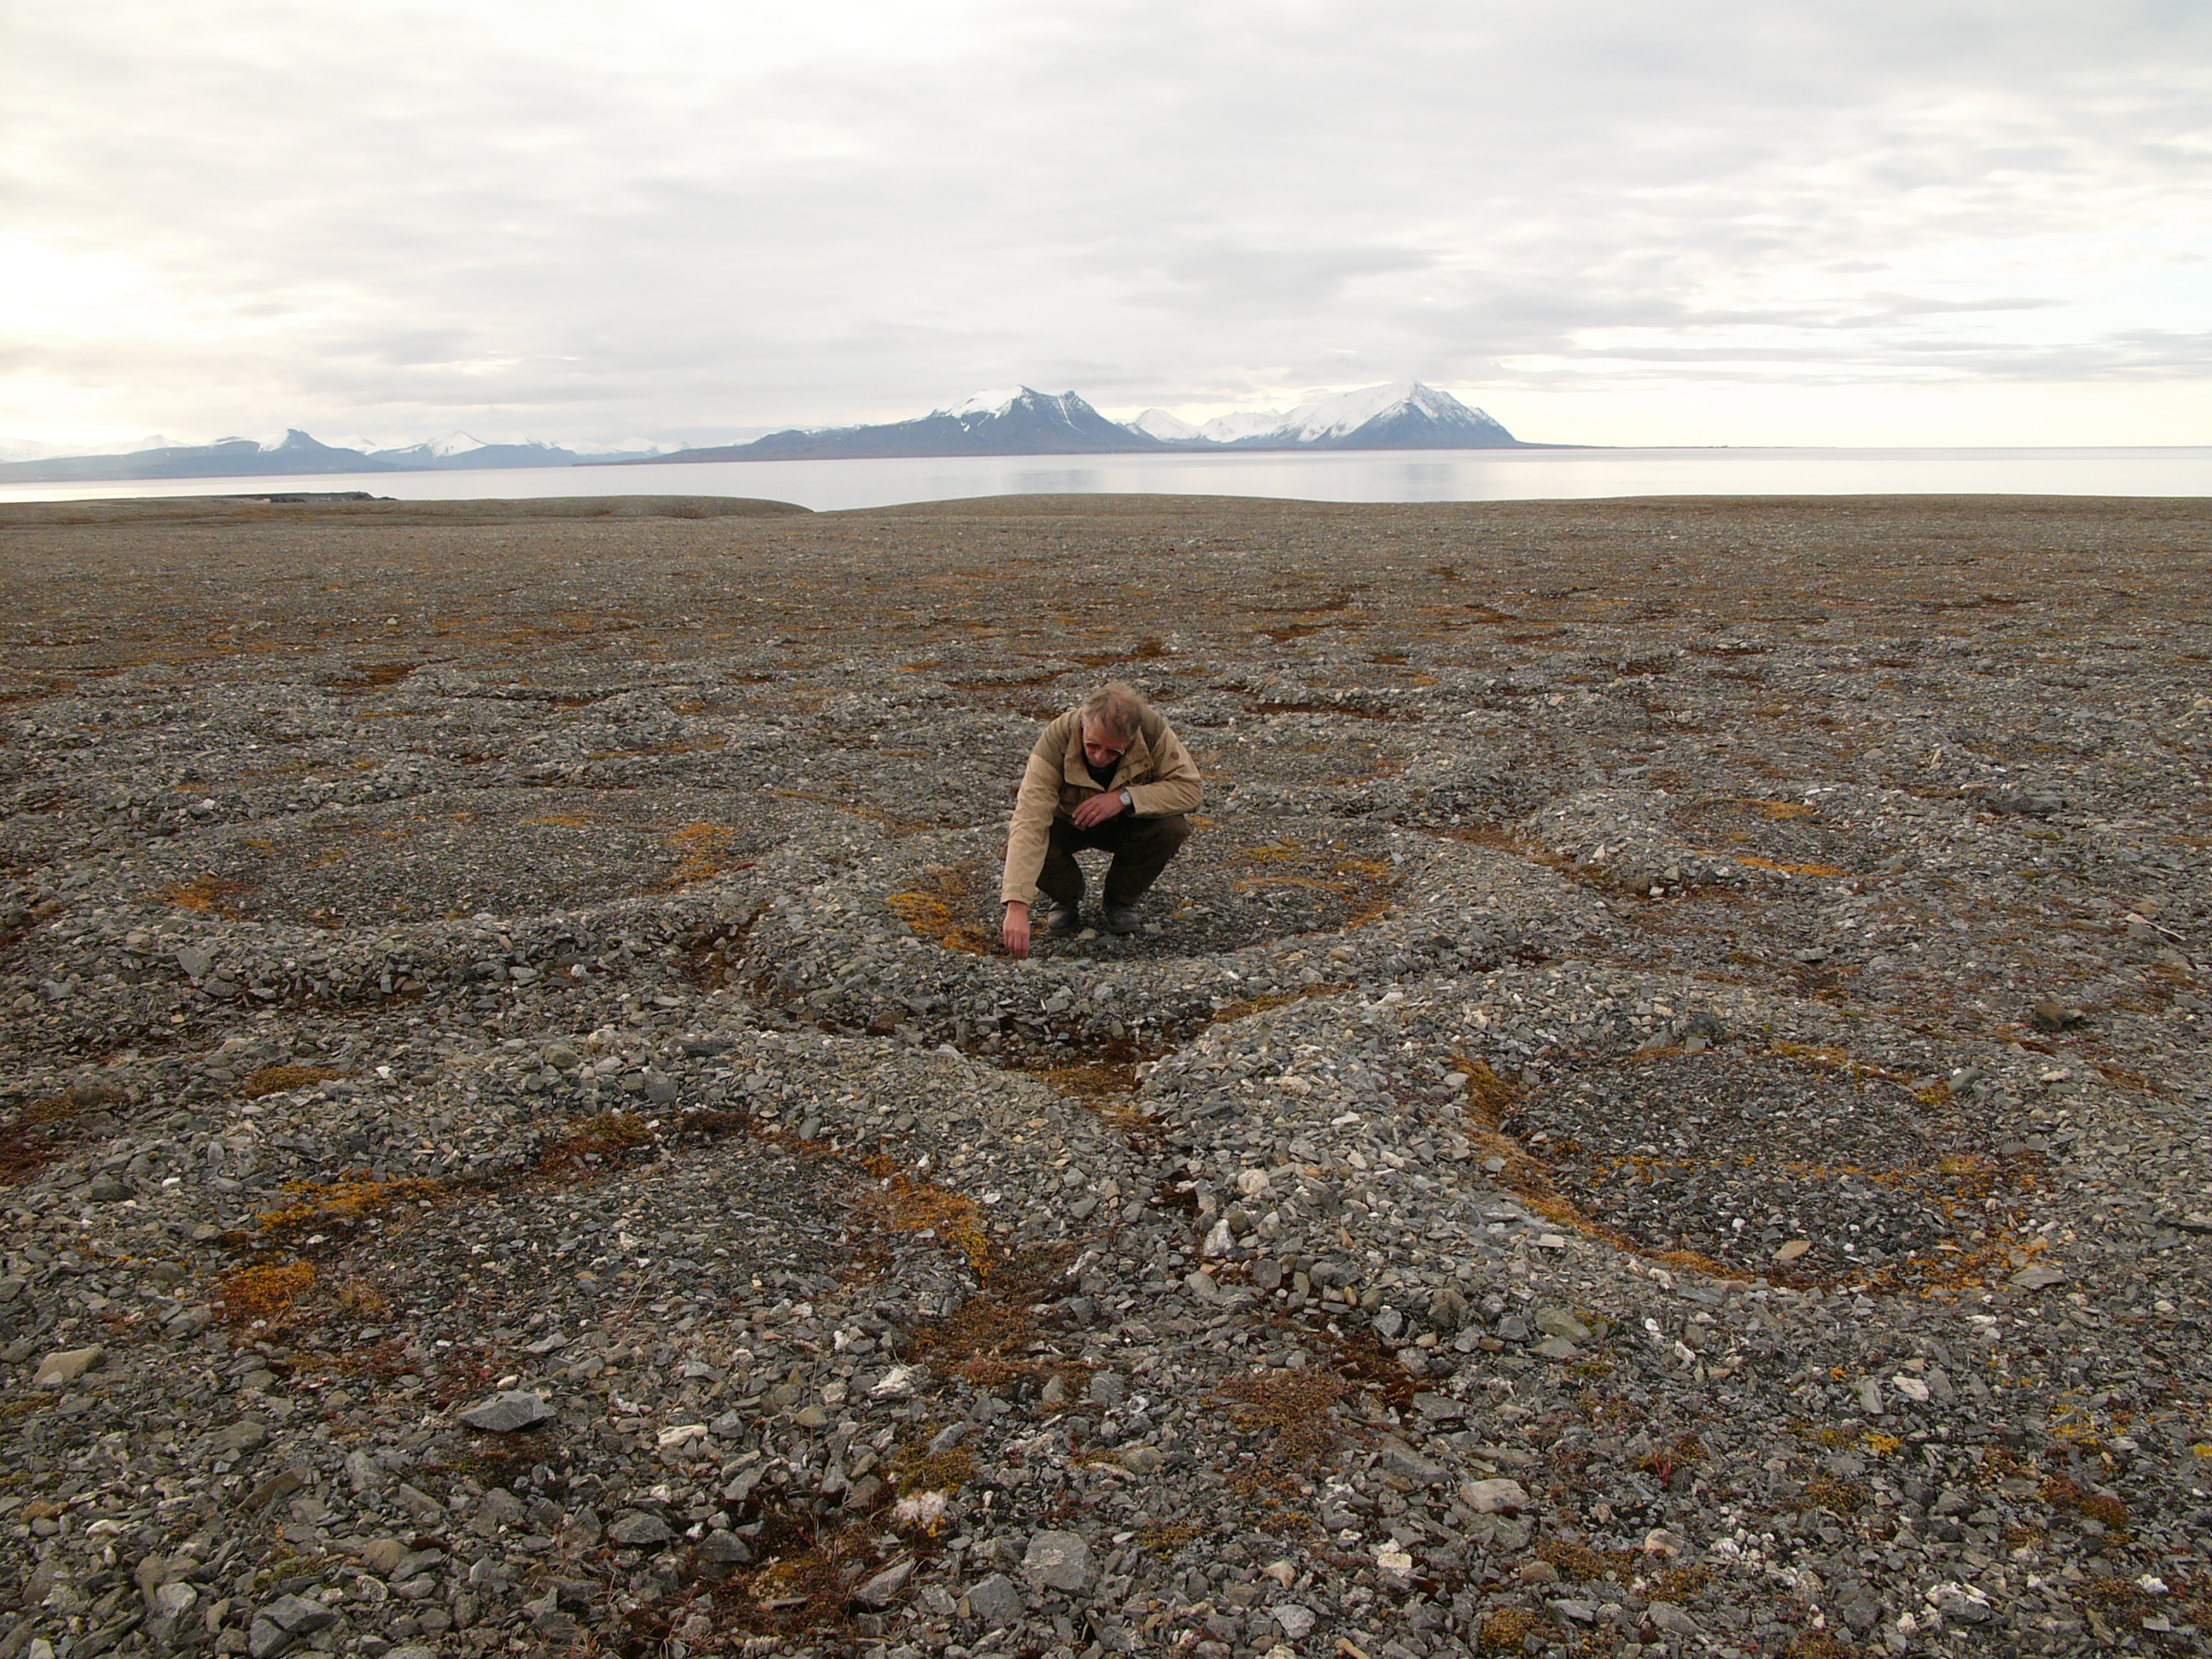
\includegraphics[trim=0 0 0.66\imagewidth{} 0, clip, width = 0.8\linewidth]{bilder/Permafrost_stone-rings_hg.jpg}
      \caption{Quelle: Wikimedia, Hannes Grobe}
    \end{figure}
    \column{.7\linewidth}
	\begin{itemize}
		\item Dauerhaft gefrorene Böden (permanent $<$ \SI{0}{\degreeCelsius})
		\item Größtenteils in Nordamerika und Eurasien
		\item Konserviert unzersetzte organische Materie
		\item [$\rightarrow$] Geschätzt 1000 Gt (1 Gt = $10^{15}$ g) Kohlenstoff gespeichert
		\item Deutliche Verschiebung der Permafrostgrenze im letzten Jahrhundert beobachtet
		\item Die globale Erwärmung gefährdet den Fortbestand des Permafrostes
		\item Folgen des Abtauens: Absenken der Böden, Überschwemmungen, Zersetzung bisher konservierter Materie
    \begin{itemize}
      \item[$\rightarrow$] Freisetzung großer Mengen CO$_2$ und Methan
    \end{itemize}
	\end{itemize}
\end{columns}

	\note{
		\begin{itemize}
			\item[] Tiefe des Permafrostes ist abhängig von Oberflächen-Temperatur
      \item[] Zum Teil mehrere hundert Meter tief gefroren
			\item[] In Sibirien liegt kaum Schnee, sodass die Böden noch kälteren Temperaturen ausgesetzt sind
			\item[] Verschiebung der Permafrost-Grenze in Kanada z.B um 100km nach Norden im letzten Jahrhundert
			\item[] Absinken gefährdet auch lokale Infrastruktur wie Straßen, Städte und Öl-Pipelines
			\item[] Überschwemmung gefährdet Wälder $\rightarrow$ 'ertrinken'
      \item[] Wissenschaft nimmt an, dass deutlich mehr Treibhausgase freigesetzt werden, als die erwartete neue Vegetation binden würde
		\end{itemize}
	}
\end{frame}

\begin{frame}
	\frametitle{Konsequenzen der Verringerung der Eismassen}
	\begin{itemize}
		\item Verringerter Albedo-Effekt
		\item Abgeschwächte Konvektion
		\item Abgeschwächte Ozeanströmung und Winde
		\item Anstieg des Meeresspiegels
		\item Massive Freisetzung von Treibhausgasen aus den Senken Ozean und Permafrost
		\item Trägheit führt zu verzögertem Eintreten der Änderungen
	\end{itemize}

	$\rightarrow$ Insgesamt: eine Verstärkung des Treibhauseffekt mit weiteren noch unabsehbaren Folgen

	\note{
		\begin{itemize}
			\item[] Das Schmelzen der Polkappen und Auftauen des Permafrostes ist ein deutliches Signal
			\item[] Wie gesagt, kann ein einmal in Gang gesetztes Abtauen schwer aufzuhalten sein
			\item[] Die Effekte können deutlich später auftreten
		\end{itemize}
	}
\end{frame}

\begin{frame}
	\frametitle{Vegetation}

	\begin{figure}
		\centering
		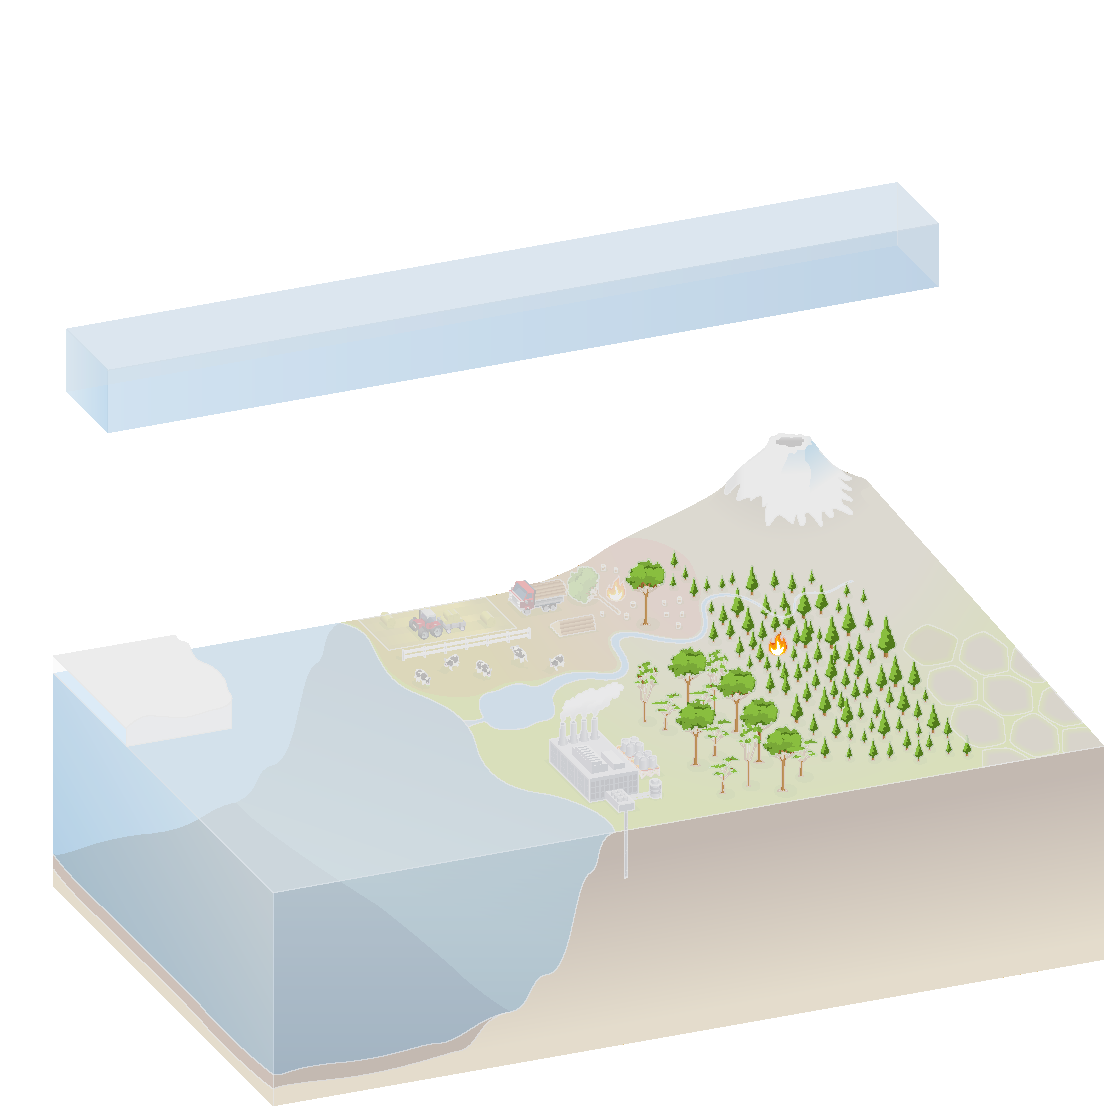
\includegraphics[trim={1cm 0cm 0cm 3cm}, clip, width=0.6\linewidth]{%
        bilder/climate_components/global_climate_components_biosphere.pdf}
		\caption{Die Vegetation ist eine interaktive Komponente des Klimasystems}
	\end{figure}

	\note{
		\begin{itemize}
			\item[] Vegetation ist sehr umfangreich und vielseitig
			\item[] steht in direktem Kontakt mit unterer Atmosphäre und Böden
			\item[] durch photosynthetische Prozesse und die Aufnahme sowie Abgabe von Wasser
			\item[] Vegetation hat dadurch massiven Einfluss auf Wetter und Klima - z.B. Tropischer Regenwald, Wolkenbildung
			\item[] zentral ist auch die Rolle beim Stoffkreislauf - u.a. Kohlenstoff, Phosphor, Nitrat, Stickstoff
			\item[] bietet Lebensraum und Lebensgrundlage
		\end{itemize}
	}
\end{frame}

\begin{frame}
	\frametitle{Pedosphäre - Böden}

	\begin{figure}
		\centering
		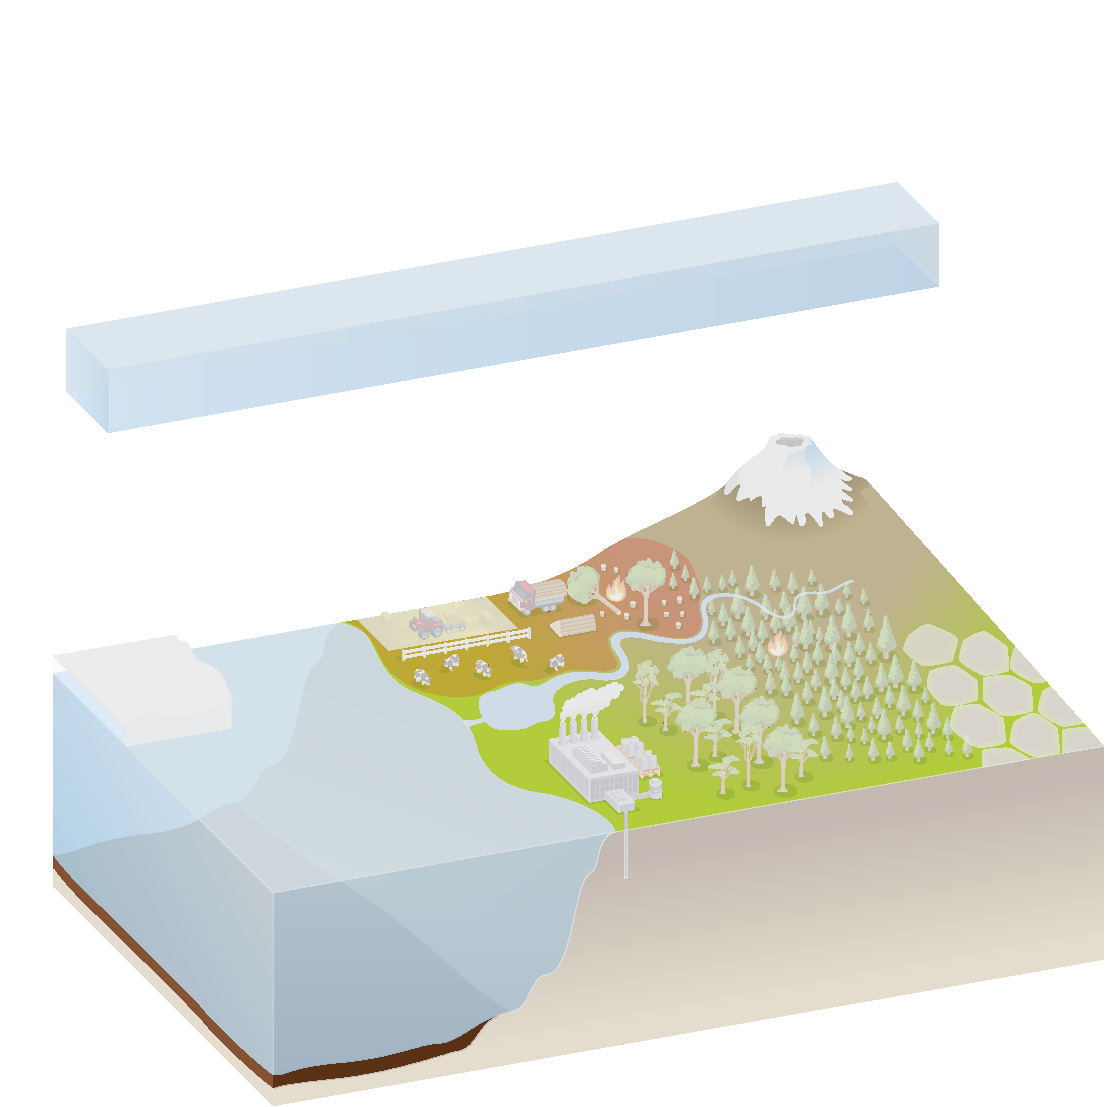
\includegraphics[trim={1cm 0cm 0cm 3cm}, clip, width=0.55\linewidth]{%
        bilder/climate_components/global_climate_components_pedosphere.pdf}
		\caption{Die Pedosphäre bezeichnet ist der Bereich der Erdoberfläche in dem sich Lithosphäre, Hydrosphäre, Atmosphäre und Biosphäre überschneiden.}
	\end{figure}

	\note{
		\begin{itemize}
			\item[] Boden
		\end{itemize}
	}
\end{frame}

\begin{frame}
	\frametitle{Lithosphäre - Gestein}

	\begin{figure}
		\centering
		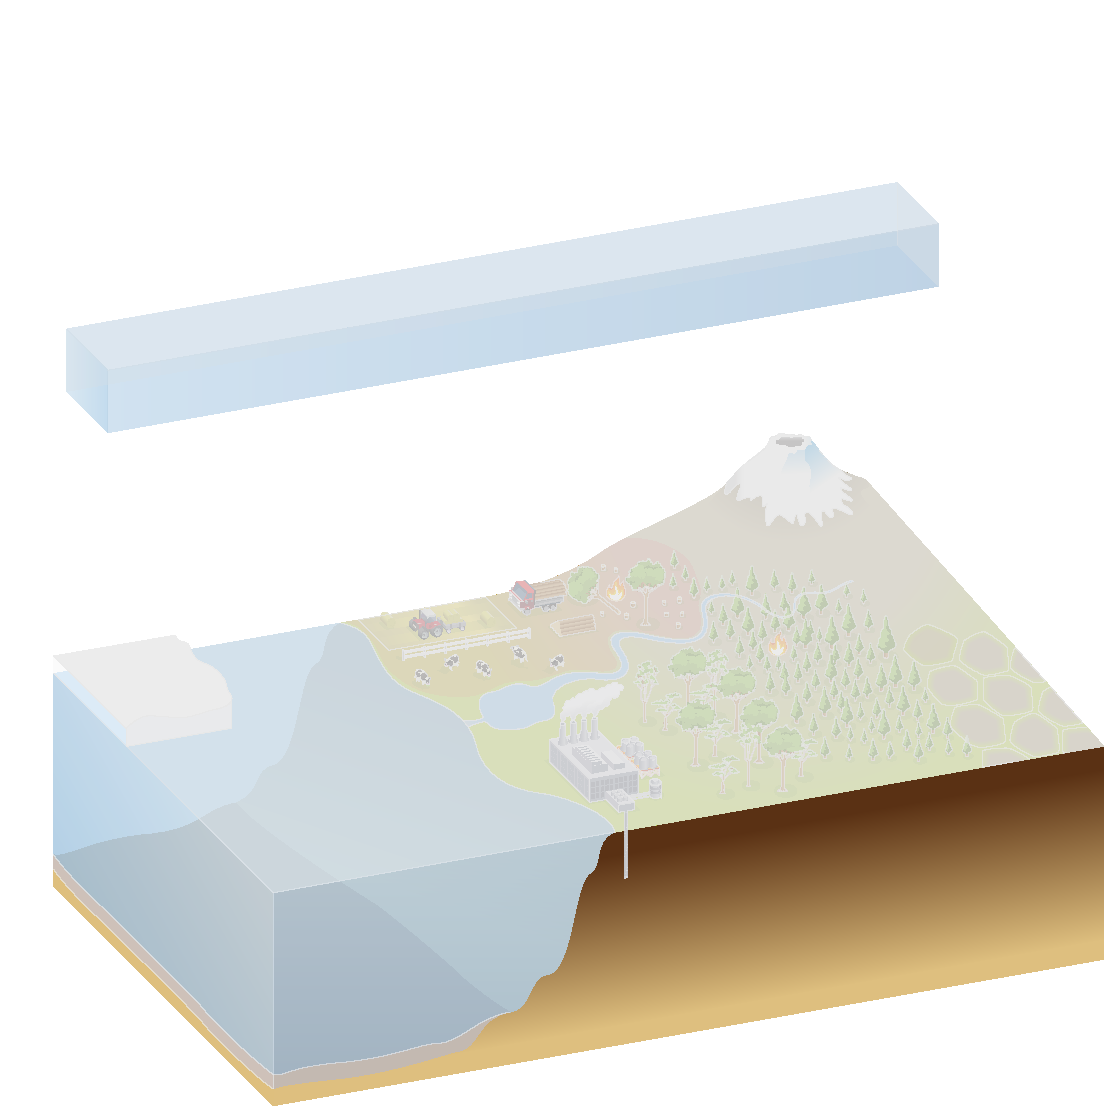
\includegraphics[trim={1cm 0cm 0cm 3cm}, clip, width=0.55\linewidth]{%
        bilder/climate_components/global_climate_components_lithosphere.pdf}
		\caption{Die Lithosphäre besteht aus der Erdkruste und dem relativ starren Teil des oberen Erdmantels.}
	\end{figure}

	\note{
		\begin{itemize}
			\item[] Gestein
		\end{itemize}
	}
\end{frame}

\subsection{Interaktionen der Faktoren des Klimasystems}
\begin{frame}
	\frametitle{Eis-Albedo-Rückkopplung}%Rahmstorf, Schellnhuber - Der Klimawandel S. 14
  \begin{center}
	 Reflexion der ankommenden Sonneneinstrahlung durch Eismassen\\[3em]
 \end{center}

	 \begin{columns}[T] % align columns
	 	\begin{column}{.48\textwidth}
	 		\centering
	 		\textbf{Abkühlung}\\
	 		\color{blue}\rule{\linewidth}{4pt}
	 		\color{black}
	 		\color<2->{gray}
	 		je mehr Eismassen\\
	 		$\downarrow$\\
	 		desto mehr wird reflektiert/\\
	 		desto weniger wird absorbiert\\
	 		$\downarrow$\\
	 		desto kälter wird es auf dem Planeten\\
	 		$\downarrow$\\
	 		desto weniger Wasserdampf kann die Atmosphäre aufnehmen\\
	 		$\downarrow$\\
	 		desto geringer wird der Treibhauseffekt
	 	\end{column}%
	 	\hfill%
	 	\begin{column}{.48\textwidth}<2->
	 		\centering
	 		\textbf{Aufwärmung}\\
	 		\color{red}\rule{\linewidth}{4pt}
	 		\color{black}
	 		je weniger Eismassen\\
	 		$\downarrow$\\
	 		desto weniger wird reflektiert/\\
	 		desto mehr wird absorbiert\\
	 		$\downarrow$\\
	 		desto wärmer wird es auf dem Planeten\\
	 		$\downarrow$\\
	 		desto mehr Wasserdampf kann die Atmosphäre aufnehmen\\
	 		$\downarrow$\\
	 		desto stärker wird der Treibhauseffekt
	 	\end{column}%
	 \end{columns}
\note{
\begin{itemize}
	\item[] hier wird die genannten Wechselwirkung unterschiedlicher Faktoren am Beispiel Eis-Albedo Rückkoppelung erläutert
	\item[] Albedo ist im wesentlichen das Reflexionsvermögen eines Körpers auf einer Skala von 0 bis 1, eine hohe Albedo bedeutet viel Reflexion
	\item[] I.a. gibt es viele ähnliche Rückkoppelungen im Klimasystem, z.B. auch bei Landnutzung/Grünflächen und kann im Prinzip sowohl positiv wie negativ sein
	\item[] Negative Rückkoplung führt zu einem stabilen Verhalten, positive Rückkopplung zu schwer kontrolierbarem Anwachsen.
  \end{itemize}
  }

\end{frame}

% "Runterscrollen" / "Zoom" in einer Abbildung von den Atmosphärischen Schichten auf die Erde

\begin{frame}
	\frametitle{Interaktion Hydrosphäre, Kryosphäre und Atmosphäre}
	\begin{columns}
		\column{.6\linewidth}
		\begin{figure}
			\centering
			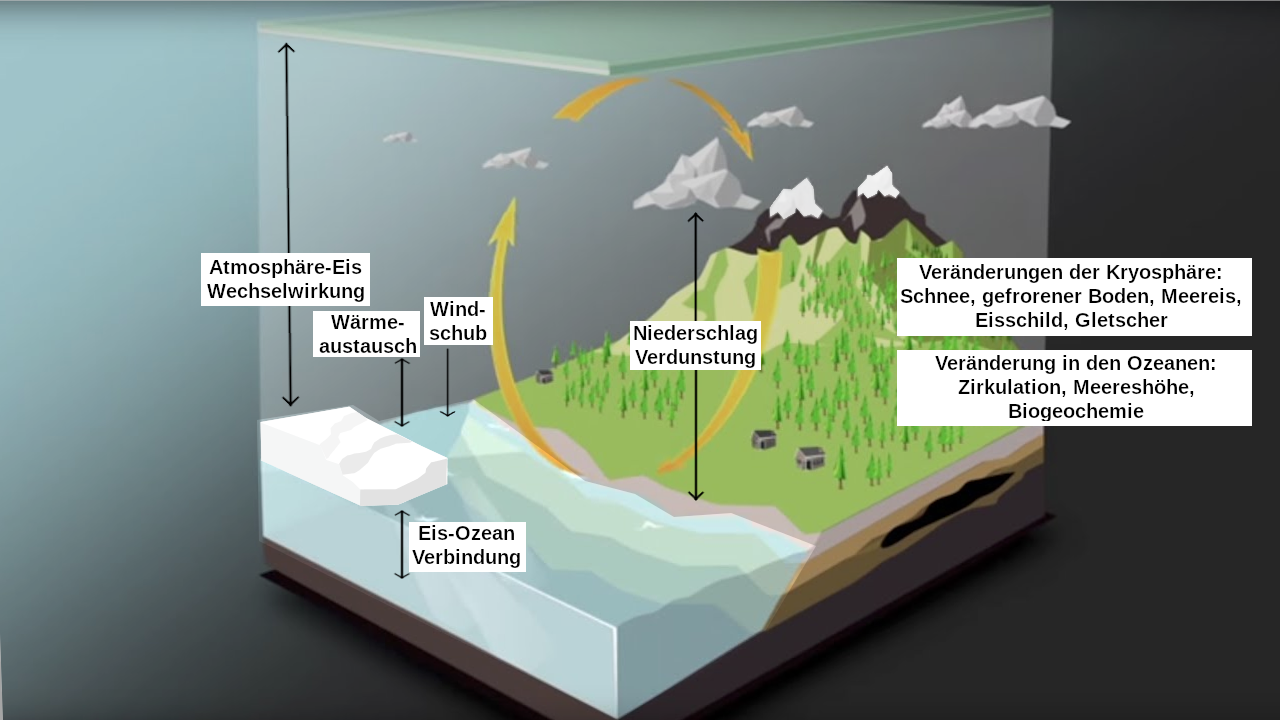
\includegraphics[width=\linewidth]{bilder/WMO_Cycles_factors_waterAndIce.png}
			\caption{Interaktion Hydrosphäre, Kryosphäre und Atmosphäre}
		\end{figure}
		\column{.4\linewidth}
		\begin{itemize}
			\item Verringerter Albedo-Effekt
			\item Abgeschwächte Konvektion
			\item Abgeschwächte Ozeanströmung und Winde
			\item Anstieg des Meeresspiegels
			\item Massive Freisetzung von Treibhausgasen aus den Senken Ozean und Permafrost
			\item Trägheit führt zu verzögertem Eintreten der Änderungen
		\end{itemize}
	\end{columns}
	\begin{block}{}
			$\rightarrow$ Insgesamt: eine Verstärkung des Treibhauseffekt mit weiteren noch unabsehbaren Folgen
	\end{block}

	\note{
		\begin{itemize}
			\item[] links an den Pfeilen sind die Wechselwirkungen notiert - z.B. Eis-Ozean-Verbindung (Konvektion)
			\item[] rechts sieht man die allgemeinen Elemente der Komponenten Hydrosphäre und Kryosphäre
			\item[] diese Elemente hängen offensichtlich zusammen und bedingen sich gegenseitig
			\item[] Das Schmelzen der Polkappen und Auftauen des Permafrostes ist ein deutliches Signal
			\item[] Wie gesagt, kann ein einmal in Gang gesetztes Abtauen schwer aufzuhalten sein
			\item[] Die Effekte können deutlich später auftreten
		\end{itemize}
	}
\end{frame}

\begin{frame}
	\frametitle{Interaktion Vegetation und Atmosphäre}

  \begin{figure}
    \centering
    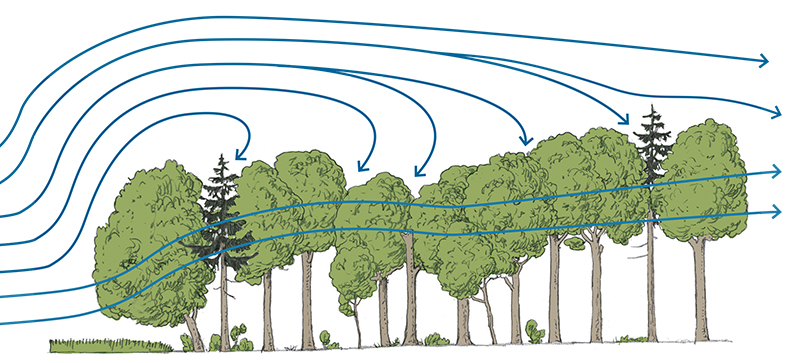
\includegraphics[width=.55\linewidth]{bilder/Wind_Vegetation.jpg}
    \caption{Wechselwirkung zwischen Atmosphäre und Biosphäre, Quelle: Stadt Kriens}
  \end{figure}
		\begin{itemize}
			\item Bodenbedeckung wirkt auf Wind, Wasseraustausch und Strahlungshaushalt
			\item [$\rightarrow$] Wälder bremsen Winde, speichern Wasser, beeinflussen Wolkenbildung und bilden Schatten und großen Lebensraum
			\item [$\rightarrow$] in Wüsten und Steppen versickert Wasser schneller und es gibt kaum Schatten, dafür existiert schwacher Albedo-Effekt
			\item Existenz und Wachstum von Vegetation bindet u.a. CO$_2$ und absorbiert Strahlung
			\item Absterben von Vegetation führt zu Freisetzung von CO$_2$ und anderen Stoffen in die Luft und Böden % Nitrat, Phosphat, Stickstoff etc.
		\end{itemize}

	\note{
		\begin{itemize}
			\item[] Photosynthese: Aufnahme von CO$_2$ und abgabe von O$_2$, Nutzung des Kohlenstoff für das Wachstum
			\item[] Lösung organischer Kohlenstoff-Verbindungen durch baterielle Zersetzung $\rightarrow$ Freisetzung von CO$_2$
			\item[] Änderungen an der Landoberfläche durch z.B: Änderung der Landnutzung - Waldrodung, Landwirtschaft ändern auch die Vegetation und die Ökosysteme
		\end{itemize}
		Fragen? Sonst $\rightarrow$ Klimamodelle
	}
\end{frame}

%\begin{frame}
%	\frametitle{Interaktion Vegetation und Atmosphäre}
%
%		\begin{figure}
%		\centering
%		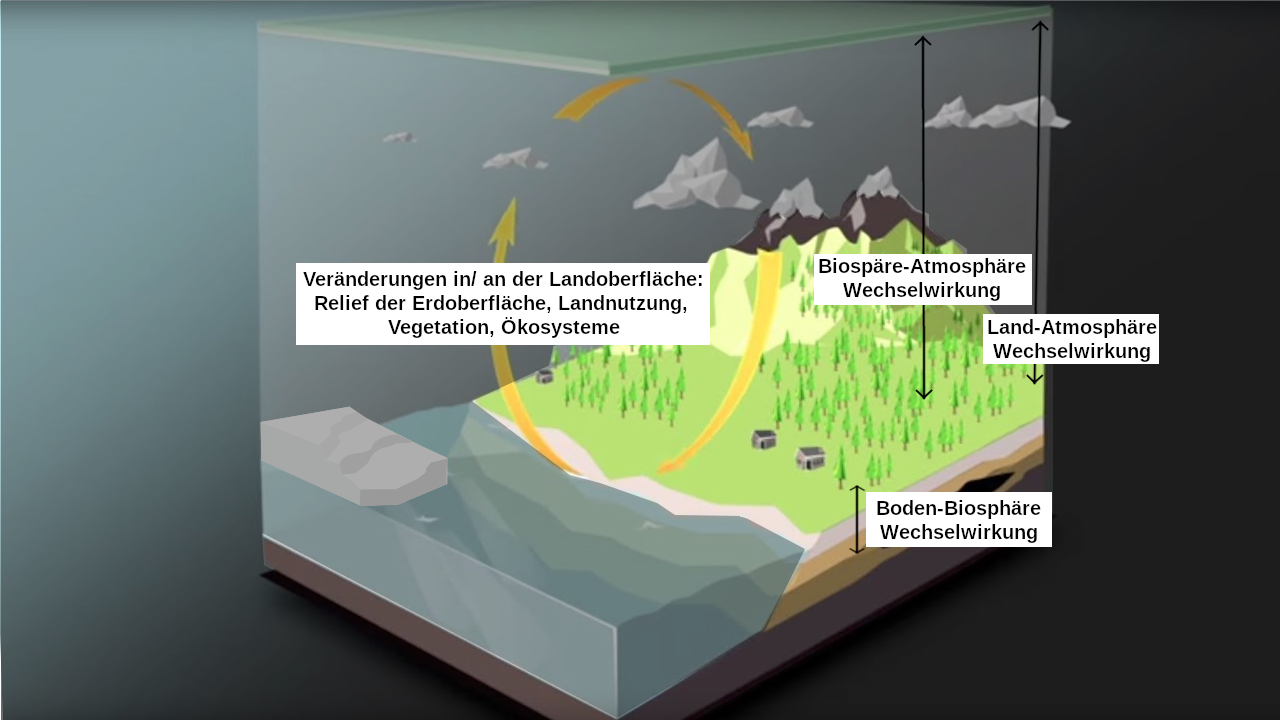
\includegraphics{bilder/WMO_Cycles_factors_landAndGround.png}
%		\caption{Interaktion der Biosphäre und Atmosphäre}
%	\end{figure}
%
%	\note{
%		\begin{itemize}
%			\item[] diesmal sind rechts die Wechselwirkungen der Vegetation und %Biosphäre zu sehen
%			\item[] links sind nochmal die zentralen Elemente der Komponente %Vegetation aufgelistet
%		\end{itemize}
%	}
%\end{frame}

\subsection{Zusammenfassung}
\begin{frame}
	\frametitle{Das Klimasystem - Zusammenfassung}

	\begin{figure}
		\centering
		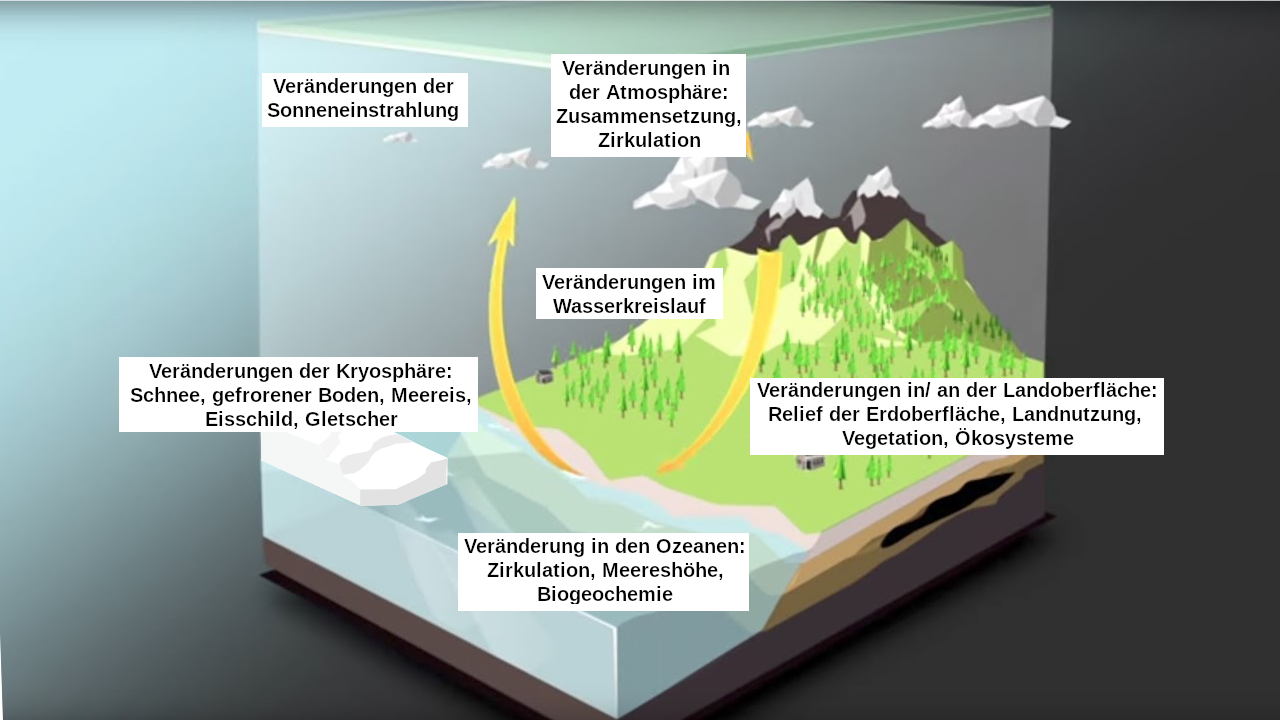
\includegraphics{bilder/WMO_Cycles_overview.png}
		\caption{Abbildung des Klimasystems mit allen zuvor erklärten Elementen}
	\end{figure}

	\note{
		\begin{itemize}
			\item[] Abbildung mit allen zuvor erklärten Elementen
			\item[] das sind nur die größten Komponenten,
			\item[] viele kleinere Bereiche wie die Böden oder Elemente wie bestimmte Stoffkreisläufe sind ebenfalls wichtig
			\item[] es ist ein sehr komplexes System, an dem in vielen Stellen Änderungen und Wechselwirkungen auftreten
			\item[] also: komplexes System, mit komplexen Zusammenhängen
			\item[] in einzelnen Bereichen wie der Wolkenbildung sind noch Forschungsfragen offen
			\item[] (wir wollen Klarheit reinbringen, damit Lösungen eher im Kontext betrachtet werden können)
			\item[] (Eine Lösung kann nämlich Rückkopplungseffekte in anderen Bereichen erzeugen)
		\end{itemize}
	}
\end{frame}


	\subsection{Kohlenstoffkreislauf}

\begin{frame}
	\frametitle{Kohlenstoffkreislauf}
	\begin{columns}
		\column{0.25\linewidth}
		\begin{figure}
			\centering
			
\includegraphics[width=\linewidth]{bilder/kohlenstoff/Brillanten}
			\caption{Diamant, 100\% Kohlenstoff, Bildquelle: Wiki1}
		\end{figure}
		\column{0.25\linewidth}
		\begin{figure}
			\centering
			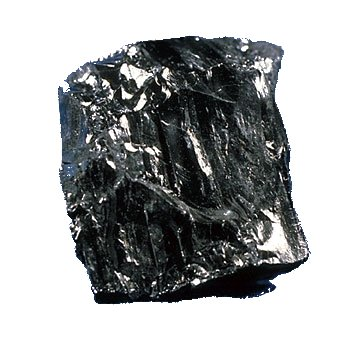
\includegraphics[width=\linewidth]{bilder/kohlenstoff/kohle}
			\caption{Anthrazit Kohle, $\geq\,90$\% Kohlenstoff (trocken), Bildquelle: Wiki2}
		\end{figure}
		\column{0.25\linewidth}
		\begin{figure}
			\centering
			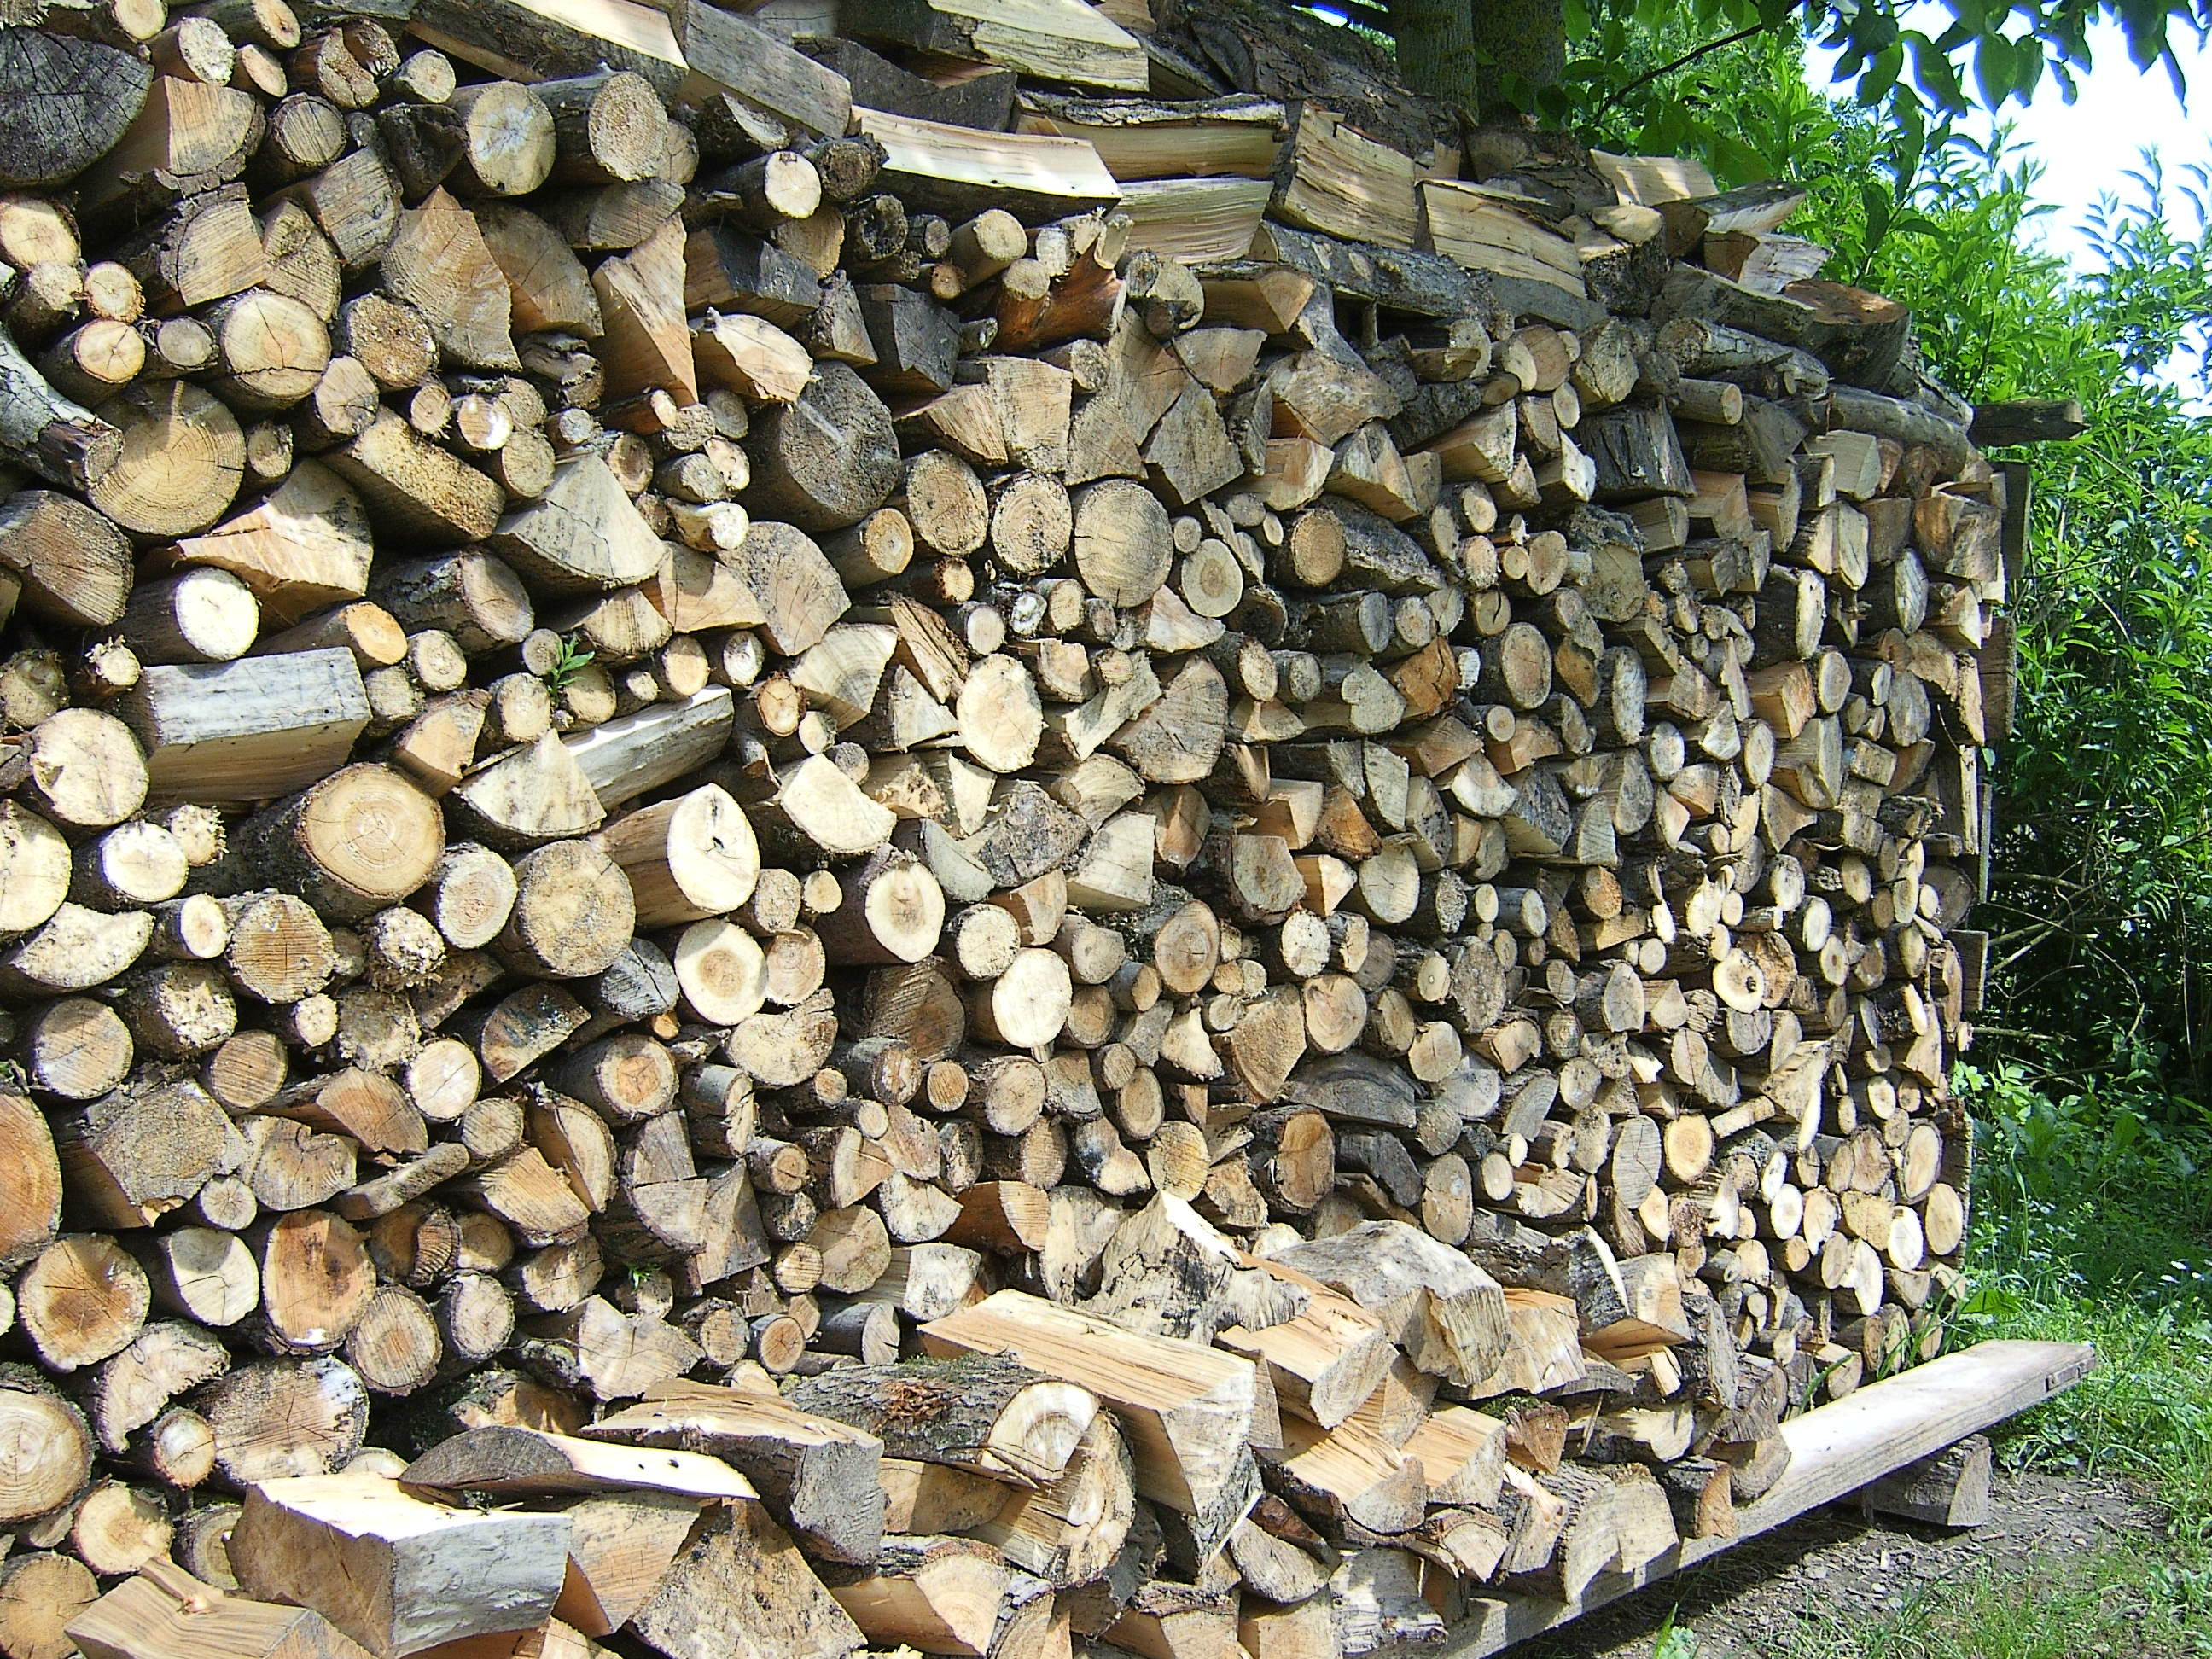
\includegraphics[width=\linewidth]{bilder/kohlenstoff/holz}
			\caption{Holz, $\approx 50$\% Kohlenstoff (trocken), Bildquelle: Wiki3}
		\end{figure}
		\column{0.25\linewidth}
		\begin{figure}
			\centering
			
\includegraphics[width=\linewidth]{bilder/kohlenstoff/co2}
			\caption{Kohlenstoffdioxid $\text{CO}_2$, Ein Kohlenstoff und zwei Sauerstoff Atome, Bildquelle: Wiki4}
		\end{figure}
	\end{columns}
		\begin{itemize}
			\item Kohlenstoff als reiner Stoff (Diamant, Graphit) oder als Verbindung mit anderen Elementen
			\item Kohlenstoff ist ein Grundbaustein des Lebens
			\item Grundlage der organischen Chemie
			\item Ist Bestandteil von Pflanzen und Tieren
			\item Im Boden gebunden und als Gas in der Atmosphäre
		\end{itemize}

	\note{
		\begin{itemize}
			\item[] Was ist das chemische Element Kohlenstoff überhaupt?
			\item[] Angaben in Massenanteilen
		\end{itemize}
	}
\end{frame}

\begin{frame}
	\frametitle{Kohlenstoffkreislauf}
	\begin{columns}
		\column{0.6\linewidth}
		\begin{figure}
			\centering
			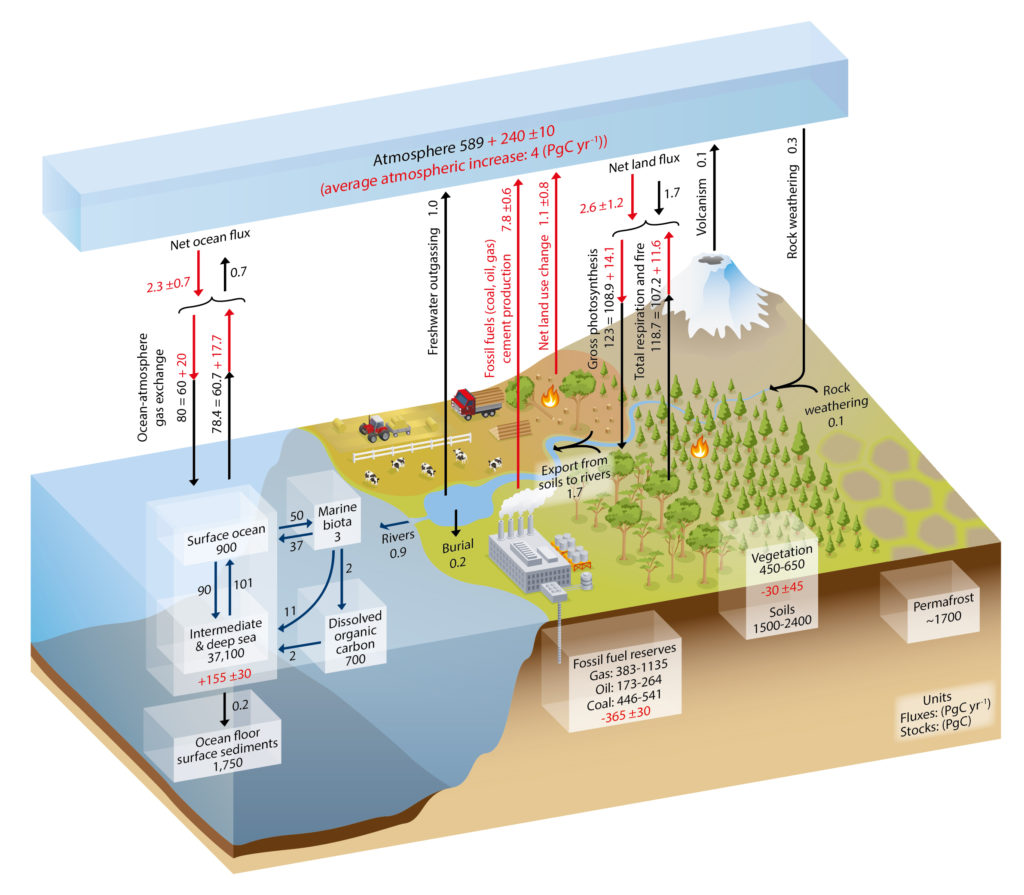
\includegraphics[width=0.9\linewidth]{bilder/IPCC_Cycles_carbon.jpg}
			\caption{Vereinfachte Abbildung zum jährlichen Kohlenstoffkreislauf, Quelle: IPCC 2013, Kapitel 6}
		\end{figure}
		\column{0.4\linewidth}
		$\Rightarrow$ vermutete natürliche CO$_2$-Flüsse vor der Industrialisierung (vor 1750)\\
		\color{red}$\Rightarrow${ }\color{black} durch Menschen verursachte mittlere jährliche CO$_2$-Flüsse (2000 - 2009) \\
		\color{red}\textbf{rote Reservoire}\color{black}: kumulative Änderung zwischen 1750 und 2011
		\begin{center}
			$\downarrow$
		\end{center}
		\textbf{der Kohlenstoffgehalt der Atmosphäre steigt um ca. 4 Gt pro Jahr}
	\end{columns}


	\note{
		\begin{itemize}
			\item[] Die Abbildung ist aus dem neusten IPCC report 2013
			\item[] Sie zeigt die Kohlenstoff-Flüsse schematisch
			\item[] schwarze Pfeile sind die geschätzten jährlichen Emissionen vor der Industrialisierung - also vor 1750
			\item[] rote Pfeile sind die mittleren jährlichen Emissionen zwischen 2000 und 2009
			\item[] Die Kohlenstoff-Speicher in der Erde und der Atmosphäre sind aber die geschätzten \textbf{gesamten Vorkommen}
			\item[] die gesamten Änderungen seit der Industrialisierung sind hierbei wieder \textbf{rot}
			\item[] v.a. aus fossilen Brennstoffen 7,8 Pg C (1 Pg = \num{e15} g)
			\item[] wird im Ozean gespeichert $\rightarrow$ Konvektion

			\item[] \textbf{Fazit: der CO$_2$ Gehalt der Atmosphäre hat sich seit der Industrialisierung beinahe verdoppelt}
			\item[] es ist anzunehmen, dass die Werte heute nochmal höher sind als die angegebenen von 2000-2009
		\end{itemize}
	}
\end{frame}
\begin{frame}
	\frametitle{Kohlenstoffkreislauf}
	\begin{columns}
		\column{0.6\linewidth}
		\begin{figure}
			\centering
			\includegraphics[width=0.9\linewidth]{bilder/kohlenstoff/cycle_reservoirs.png}
			\caption{Kohlenstoff-Speicher in Erde und Atmosphäre.}
		\end{figure}
		\column{0.4\linewidth}
		\begin{itemize}
			\item [] \textbf{Schwarze Zahlen} beschreiben gesamte geschätze Vorkommen in den jeweiligen Reservoiren.
		\end{itemize}

	\end{columns}

\end{frame}



\begin{frame}
	\frametitle{Kohlenstoffkreislauf}
	\begin{columns}
		\column{0.6\linewidth}
		\begin{figure}
			\centering
			\includegraphics[width=0.9\linewidth]{bilder/kohlenstoff/cycle_arrows-ocean-and-atmosphere.png}
			\caption{Wechselwirkungen zwischen Ozeanen und Atmosphäre.}
		\end{figure}
		\column{0.4\linewidth}
		\begin{itemize}
			\item [] \textbf{Schwarze \rightarrow} sind geschätzte natürliche CO$_2$-Flüsse vor der Industrialisierung (vor 1750)
		\end{itemize}
	\end{columns}
\end{frame}

\begin{frame}
	\frametitle{Kohlenstoffkreislauf}
	\begin{columns}
		\column{0.6\linewidth}
		\begin{figure}
			\centering
			\includegraphics[width=0.9\linewidth]{bilder/kohlenstoff/cycle_arrows-land-and-atmosphere.png}
			\caption{Wechselwirkungen zwischen Landmassen und Atmosphäre.}
		\end{figure}
		\column{0.4\linewidth}
		\begin{itemize}
			\item [] \textbf{Schwarze \rightarrow} sind geschätzte natürliche CO$_2$-Flüsse vor der Industrialisierung (vor 1750)
		\end{itemize}
	\end{columns}
\end{frame}


\begin{frame}
	\frametitle{Kohlenstoffkreislauf}
	\begin{columns}
		\column{0.6\linewidth}
		\begin{figure}
			\centering
			\includegraphics[width=0.9\linewidth]{bilder/kohlenstoff/cycle_antropogenic-ocean-and-atmosphere.png}
			\caption{Anthropogener Einfluss im Kreislauf zwischen Ozeanen und Atmosphäre.}
		\end{figure}
		\column{0.4\linewidth}
		\begin{itemize}
			\item \color{red}\textbf{Rote \rightarrow} \color{black} sind durch Menschen verursachte mittlere jährliche CO$_2$-Flüsse von zwischen 2000 und 2009.
			\item \color{red}\textbf{Rote Reservoire} \color{black} sind die kumulative Änderung zwischen 1750 und 2011.
		\end{itemize}
	\end{columns}
\end{frame}

\begin{frame}
	\frametitle{Kohlenstoffkreislauf}
	\begin{columns}
		\column{0.6\linewidth}
		\begin{figure}
			\centering
			\includegraphics[width=0.9\linewidth]{bilder/kohlenstoff/cycle_antropogenic-ocean-and-atmosphere.png}
			\caption{Anthropogener Einfluss im Kreislauf zwischen Landmassen und Atmosphäre.}
		\end{figure}
		\column{0.4\linewidth}
		\begin{itemize}
			\item \color{red}\textbf{Rote \rightarrow} \color{black} sind durch Menschen verursachte mittlere jährliche CO$_2$-Flüsse von zwischen 2000 und 2009.
			\item \color{red}\textbf{Rote Reservoire} \color{black} sind die kumulative Änderung zwischen 1750 und 2011.
		\end{itemize}
	\end{columns}
\end{frame}

\begin{frame}
	\frametitle{Kohlenstoffkreislauf - Der Faktor Mensch}
	\begin{itemize}
		\item CO$_2$ ist das wichtigste Spurengas des menschengemachten Treibhauseffekts
		\item es gelangt durch Verbrennung fossiler Brennstoffe vermehrt in die Atmosphäre
		\item ca. 80\% der gestiegenen CO$_2$ Konzentration der Atmosphäre lassen sich auf Verbrennung zurückführen
		\item der restliche Anteil entfällt auf die Änderung der Landnutzung, v.a. die Brandrodung
		\item Rückführung auf den Menschen durch Messung von Kohlenstoffisotopen (Anzahl Neutronen in einem Kohlenstoffatom)
		\item[$\rightarrow$] das Verhältnis der Isotope in fossilen Brennstoffen hat durch die Verbrennung Einfluss auf das Verhältnis in der Atmosphäre
	\end{itemize}

	\note{
		\begin{itemize}
			\item[] Verschiedene Isotope haben unterschiedliche Massen
			\item[] Isotopmessung:  $^{12}$C hat sechs und $^{13}$C sieben Neutronen, beide haben 6 Protonen, die den Kohlenstoff kennzeichnen
			\item[] Fossile Brennstoffe haben ein geringes $^{13}$C zu $^{12}$C Verhältnis
			\item[] durch die Verbrennung entsteht aus organischen $^{12}$C und $^{13}$C CO$_2$ mit entsprechenden Isotopen
			\item[] Sinkt das Isotopenverhältnis in der Atmosphäre, muss also das CO$_2$ aus Verbrennung fossiler Brennstoffe kommen
			\item[] Zusätzlich: Sauerstoffkonzentration messen, da der Sauerstoff für CO$_2$ aus der Atmosphäre stammt
			\item[$\rightarrow$] Sinkt sie in einem festen Verhältnis zur CO$_2$ Zunahme erhärtet das den Verdacht menschlichen Einflusses
			\item[] Übergang nächste Folie: Aber nicht nur der CO$_2$ Gehalt der Atmosphäre hat sich erhöht, sondern auch der von Methan und Lachgas
		\end{itemize}
	}
\end{frame}


\begin{frame}
	\frametitle{Atmosphärisches Methan}
	\begin{columns}
		\column{0.65\linewidth}
			\begin{figure}
				\centering
				\includegraphics[width=0.9\linewidth]{bilder/IPCC_Cycles_methane.jpg}
				\caption{Vereinfachte Abbildung zum Methankreislauf, Quelle: IPCC 2013, Kapitel 6}
			\end{figure}
		\column{0.35\linewidth}
			Der Gehalt an Methan in der Atmosphäre hat sich zwischen 1750 und 2011 um \SI{250}{\%} erhöht.
	\end{columns}

	\note{
		\begin{itemize}
			\item[] Auch diese Abbildung ist aus dem IPCC Report von 2013
			\item[] schwarze Pfeile stellen wieder vorindustrielle jährliche Flüsse dar
			\item[] rote Pfeile wieder mittlere jährliche Flüsse zwischen 2000 und 2009
			\item[] Die Speicher/Reservoire sind auch wieder als \textbf{Gesamtwert} angegeben
			\item[] vorindustielles Methan in der Atmosphäre: 1984, heutig: +2970 $\rightarrow$ insgesamt also 4954 Tg Methan
			\item[] Methan: järliches atmosphärisches Plus: 17 (+-9) Tg
			\item[] zusätzliches Methan wird freigesetzt durch:
			\begin{itemize}
				\item[] Fossile Brennstoffe: 85-105 Tg
				\item[] Massentierhaltung: 87-94 Tg
				\item[] ganz stark aus Müllhalden (land fills): 67 - 90 Tg
				\item[] $\rightarrow$ durch den anaeroben Abbau der dort gelagerten Stoffe wird von den Mikroorganismen Methan freigesetzt
				\item[] und auch Reisanbau: 33-40 Tg
			\end{itemize}
			\item[] die globalen Speicher von Methan in der Erde sind zusätzlich sehr groß: z.B. Ozean bis zu 8 Mio Tg Methan
		\end{itemize}
	}

\end{frame}

\begin{frame}
	\frametitle{Atmosphärisches Lachgas}
	\begin{columns}
		\column{0.75\linewidth}
			\begin{figure}
				\includegraphics[width=0.9\linewidth]{bilder/IPCC_Cycles_n2o_new.jpg}
				\caption{Vereinfachte Abbildung zum Lachgaskreislauf, Quelle: IPCC 2013, Kapitel 6}
			\end{figure}
		\column{0.25\linewidth}
			Der Gehalt an Lachgas in der Atmosphäre hat sich zwischen 1750 und 2011 um 20 \,\% erhöht.
	\end{columns}

	\note{
		\begin{itemize}
			\item[] Auch diese Abbildung ist aus dem IPCC Report von 2013
			\item[] vorindustielles Lachgas in der Atmosphäre: 1340, heutig: + 213 $\rightarrow$ insgesamt 1553 Tg N$_2$O
			\item[] Lachgas: järliches atmosphärisches Plus: 3,6 (+-0,15) Tg
			\item[] Lachgas v.a. aus Landwirtschaft (4,1 Tg jährliche Emissionen) Verbrennung von Biomasse und Waldrodung

			\item[] \textbf{Fazit:} durch die starke Treibhauswirksamkeit von Methan und Lachgas, sind diese Entwicklung extrem kritisch zu beobachten!
			\item[] Einsparungen in diesem Bereich würden kurzfristig helfen, durch die kürzere Verweildauer, sind sie langfristig aber exakt mit CO$_2$ zu vergleichen
		\end{itemize}
	}

\end{frame}

	\begin{frame}
	\frametitle{Zusammenfassung und Ausblick}
	\begin{figure}
		\centering
		\includegraphics[width=\linewidth]{bilder/s4f-warming-stripes}
		\caption{Die Warming Stripes}
	\end{figure}
	$\rightarrow$ Die langfristige Erwärmung und Häufung extremer Wetterereignisse bedeutet eine Veränderung des Klimas!\\
	$\rightarrow$ Viele dieser Änderungen sind in Modellen der Klimaforscher relativ genau vorherzusagen. \\
	$\rightarrow$ Das Ausmaß einiger Änderungen sind aufgrund der langfristigen Effekte nicht konkret vorherzusagen, aber die Tendenz ist klar.
\end{frame}

	\subsection{Werbeblock}
\begin{frame}
  \begin{tikzpicture}
    \onslide<1|handout:1>\node[anchor=south west,inner sep=0] (image) {\includegraphics[width=1\linewidth]{bilder/campus-for-future-vorstellung-ringvorlesung.pdf}};
    %\onslide<2|handout:1>\node[draw=yellow, fill=yellow, rotate around={-15:(0,0)}, drop shadow={color=black}, inner sep=5pt] at ($(image.center) + (4, -2.4)$) {\textbf{Klimawoche vom 23. bis 27.11.2020}};
    %\begin{scope}[x={(image.south east)},y={(image.north west)}]
      %\onslide<2|handout:1>\draw[fill=yellow, yellow, rotate around={-20:(0.625,0.25)] (0.5,0.2) rectangle (0.75,0.3) node[pos=.5] {23. bis 27.11.2020};
    %\end{scope}
  \end{tikzpicture}
\note{
  \begin{itemize}
    \item[] Link zum Discord auf Anfrage, z.B. per Mail
    \item[] C4F-Klimawoche im Rahmen  der Public Climate School 3.0 geben.
    \item[] vom 23. bis 27.11.
  \end{itemize}
}
\end{frame}

\begin{frame}
\frametitle{Scientists 4 Future Dortmund}
\begin{columns}[c] % align columns
 \begin{column}{.78\textwidth}
	 \begin{itemize}
		\item Ziel ist die Vermittlung von Fakten zum Thema Klimawandel
		\item Richtet sich an Wissenschaftler*innen in Dortmund und Umgebung
	 	\item \url{https://s4f-dortmund.github.io/}
	 \end{itemize}
 \end{column}%
 \hfill%
 \begin{column}{.28\textwidth}
	 \centering
	 ~\\~\\
		 \includegraphics[width=0.625\textwidth]{bilder/s4f_logo_dortmund.png}
 \end{column}%
\end{columns}
\begin{columns} % align columns
 \begin{column}{.48\textwidth}
	 \begin{figure}
		 \centering
		 \includegraphics[trim={0cm 0cm 0cm 2.5cm}, clip, width=0.95\textwidth]{bilder/demo.jpg}
		 \caption{S4F Dortmund beim globalem Klimastreik am 20.09.2019.}
	 \end{figure}
 \end{column}%
 \hfill%
 \begin{column}{.48\textwidth}
	 \begin{figure}
		 \centering
		 \includegraphics[width=\textwidth]{bilder/sommerkongress.jpg}
		 \caption{Workshop der S4F Dortmund beim FFF Sommerkongress.}
	 \end{figure}
 \end{column}%
\end{columns}

\note{
Dank an Mitarbeit von Robert, Sebastian und Luise, ohne die diese Vorlesung nicht möglich gewesen wäre.
}

\end{frame}

\iffalse
\begin{frame}
  \frametitle{Weitere Möglichkeiten sich zu engagieren}
  \begin{columns}
    \column{0.6\textwidth}
    \begin{figure}
      \centering
      \includegraphics[width=\textwidth]{bilder/climate-kic-logo.pdf}
    \end{figure}
    Am 13. \& 14.11.2020, weitere Infos hier: \href{https://cet.tu-dortmund.de/veranstaltungen/detail/climathon-germany-4770/}{\color{blue}\underline{Link}}\\
    Anmeldung unter:\\
    \url{https://impacthub.de/events/climathon-2020.html}
    \column{0.4\textwidth}
    \begin{figure}
      \centering
      \includegraphics[width=\textwidth]{bilder/akn-tu.jpg}
    \end{figure}
    Arbeitskreis Nachhaltigkeit der TU\\
    weitere Infos hier: \href{https://www.tu-dortmund.de/universitaet/nachhaltigkeit/}{\color{blue}\underline{Link}}
  \end{columns}

  \note{
  \begin{itemize}
    \item[] Der Climathon ist ein globaler 24-Stunden (Ideen-Marathon) für städtische Klimainnovationen.
    \begin{itemize}
      \item[] gleichzeitig in mehr als 100 Städten auf der ganzen Welt
      \item[] 1000 Kreative, Ex­per­tin­nen und Experten und Macherinnen und Macher entwickeln online gemeinsam in­no­va­ti­ve Klimaschutz-Lö­sun­gen.
      \item[] ​Ziel ist es, konkrete lokale He­raus­for­de­rung­en für mehr Klimaschutz und Klimagerechtigkeit in den Blick zu nehmen und dafür in interdisziplinär zusammengesetzten Teams Lösungsansätze entstehen zu lassen.
      \item[] Einige Challenges sind schon einsehbar
    \end{itemize}
    \item[] Arbeitskreis Nachhaltigkeit der TU Dortmund
    \begin{itemize}
      \item[] Vertreter aus Verwaltung, der Studierendenschaft und den wissenschaftlichen Mitarbeitern
      \item[] Aufgeteilt in Arbeitskreise, Mitarbeit möglich, aber Geduld nötig
    \end{itemize}
    \item[] AStA Referat Soziales, Diversität und Nachhaltigkeit
    \item[] Think Tank zur Nachhaltigkeit in der BCI
  \end{itemize}
  }
\end{frame}
\fi

	\begin{frame}
	\frametitle{Referenzen}
	\small{
	\textbf{Bildungsserver Hamburg,} Hamburger Bildungsserver (HBS), \url{https://bildungsserver.hamburg.de/klimawandel/} \\

	\textbf{IPCC, 2001:} Climate Change 2001: The Scientific Basis. Contribution of Working Group I to the Third Assessment Report of theIntergovernmental Panel on Climate Change[Houghton, J.T., Y. Ding, D.J. Griggs, M. Noguer, P.J. van der Linden, X. Dai, K.Maskell, and C.A. Johnson (eds.)]. Cambridge University Press, Cambridge, United Kingdom and New York, NY, USA, 881pp., \url{https://www.ipcc.ch/report/ar3/wg1/}\\

	\textbf{IPCC 2007:} IPCC, 2007: Climate Change 2007: The Physical Science Basis. Contribution of Working Group I to the Fourth Assessment Report of the Intergovernmental Panel on Climate Change [Solomon, S., D. Qin, M. Manning, Z. Chen, M. Marquis, K.B. Averyt, M. Tignor and H.L. Miller (eds.)]. Cambridge University Press, Cambridge, United Kingdom and New York, NY, USA, 996 pp.,  \url{https://www.ipcc.ch/report/ar4/wg1/}\\

	\textbf{IPCC, 2014:} IPCC, 2013: Climate Change 2013: The Physical Science Basis. Contribution of Working Group I to the Fifth Assessment Report of the Intergovernmental Panel on Climate Change [Stocker, T.F., D. Qin, G.-K. Plattner, M. Tignor, S.K. Allen, J. Boschung, A. Nauels, Y. Xia, V. Bex and P.M. Midgley (eds.)]. Cambridge University Press, Cambridge, United Kingdom and New York, NY, USA, 1535 pp., \url{https://www.ipcc.ch/report/ar5/wg1/}\\

	\textbf{IPCC, 2018:} IPCC, 2018: : Global warming of 1.5°C. An IPCC Special Report on the impacts of global warming of 1.5°C above pre-industrial levels and related global greenhouse gas emission pathways, in the context of strengthening the global response to the threat of climate change, sustainable development, and efforts to eradicate poverty [V. Masson-Delmotte, P. Zhai, H. O. Pörtner, D. Roberts, J. Skea, P.R. Shukla, A. Pirani, W. Moufouma-Okia, C. Péan, R. Pidcock, S. Connors, J. B. R. Matthews, Y. Chen, X. Zhou, M. I. Gomis, E. Lonnoy, T. Maycock, M. Tignor, T. Waterfield (eds.)]. In Press., \url{https://www.ipcc.ch/sr15/}\\
	}
\end{frame}

\begin{frame}
	\frametitle{Referenzen}
	\small{
	\textbf{Mojib Latif}, Klimawandel und Klimadynamik, 2009, UTB GmbH, Auflage: 1, ISBN 978-3-8252-3178-1\\
	\textbf{S4F}, Scientists for Future, \url{https://www.scientists4future.org/}\\
	\textbf{WMO}, World Meteorological Organization, Video zum Kohlenstoffkreislauf: \url{https://www.youtube.com/watch?v=E8Y6L5TI\_94}\\
	\textbf{Wiki1}, Von Mario Sarto - Selbst fotografiert, CC BY-SA 3.0, \url{https://commons.wikimedia.org/w/index.php?curid=1015397}\\
	\textbf{Wiki2}, Von \url{http://resourcescommittee.house.gov/subcommittees/emr/usgsweb/photogallery/images/Coal\%20anthracite\_jpg}, Gemeinfrei, \url{https://commons.wikimedia.org/w/index.php?curid=22263}\\
	\textbf{Wiki3}, Von Topfklao (Christoph Neumüller) at de.wikipedia - Eigenes Werk, Attribution, \url{https://commons.wikimedia.org/w/index.php?curid=4038579}\\
	\textbf{Wiki4} By Benjah-bmm27 - Own work, Public Domain, \url{https://commons.wikimedia.org/w/index.php?curid=940830}\\
	\textbf{Wiki5} Von user And1mu - modified version of, CC BY-SA 4.0, \url{https://commons.wikimedia.org/w/index.php?curid=59505315}\\
	\textbf{Wiki6} Von Stkl - Spectral lines continuous.png, Gemeinfrei, \url{https://commons.wikimedia.org/w/index.php?curid=42405328}\\
	\textbf{Wiki7} Zonobiome und Zonoökotone der Erde nach Walter und Breckle, Ökologix, nach Walter: "Vegetation und Klimazonen: Grundriß der globalen Ökologie", Ulmer, Stuttgart - 1990. ISBN 3-8001-2619-2 und Grabherr: "Farbatlas Ökosysteme der Erde", Ulmer, Stuttgart - 1997, ISBN 3-8001-3489-6 \url{https://de.wikipedia.org/wiki/Datei:Zonobiome.png}\\
	\textbf{Len}, \textit{Tipping elements in the Earth's climate system},
	Timothy M. Lenton, Hermann Held, Elmar Kriegler, Jim W. Hall, Wolfgang Lucht, Stefan Rahmstorf, and Hans Joachim Schellnhuber,
	PNAS February 12, 2008 105 (6) 1786-1793; first published February 7, 2008 https://doi.org/10.1073/pnas.0705414105
\end{frame}

\begin{frame}
	\frametitle{Referenzen}
	\small{
	\textbf{Rah}, \textit{Kipppunkte im Klimasystem - Eine kurze Übersicht},
	Stefan Rahmstorf, Anders Levermann, Ricarda Winkelmann, Jonathan Donges, Levke Caesar, Boris Sakschewski, Kirsten Thonicke,
	P\url{http://www.pik-potsdam.de/~stefan/Publications/Kipppunkte\%20im\%20Klimasystem\%20-\%20Update\%202019.pdf} \\
	\textbf{UBA} \textit{KIPP-PUNKTE IM KLIMASYSTEM - Welche Gefahren drohen?}, Umweltbundesamt Juli 2008, \url{https://www.umweltbundesamt.de/sites/default/files/medien/publikation/long/3283.pdf} (Sekundärquelle)\\
	\textbf{King} King, M.D., Howat, I.M., Candela, S.G. et al. \textit{Dynamic ice loss from the Greenland Ice Sheet driven by sustained glacier retreat}. Commun Earth Environ 1, 1 (2020). \url{https://doi.org/10.1038/s43247-020-0001-2}\\
	\textbf{Global Historical Climate Network}, Menne, M.J., I. Durre, B. Korzeniewski, S. McNeal, K. Thomas, X. Yin, S. Anthony, R. Ray, R.S. Vose, B.E.Gleason, and T.G. Houston, 2012: Global Historical Climatology Network - Daily (GHCN-Daily), Version 3, NOAA National Climatic Data Center. \url{http://doi.org/10.7289/V5D21VHZ}, images of density of weather stations from \url{https://www.ncdc.noaa.gov/ghcn-daily-description}\\
	\textbf{LSBU}, \url{http://www1.lsbu.ac.uk/water/water_phase_diagram.html}\\
	\textbf{chemga}, \url{http://www.chemgapedia.de/vsengine/vlu/vsc/de/ch/8/bc/vlu/chem_grundlagen/wasser.vlu/Page/vsc/de/ch/8/bc/chemische_grundlagen/wasser1.vscml.html}\\
	\textbf{USGS}, United States Geological Survey \url{https://de.wikipedia.org/wiki/Datei:Tectonic_plates_de.svg}\\
	\textbf{NOAA}, US National Oceanic and Atmospheric Administration \url{https://celebrating200years.noaa.gov/breakthroughs/climate_model/}\\
	}
\end{frame}


\end{document}
